\documentclass[11pt,a4paper,DIV=12,numbers=noenddot,bib=totoc]{scrreprt}

% Helvetica font
%\usepackage[scaled]{helvet}
%\renewcommand{\familydefault}{\sfdefault}

% Set line spacing to match previous 11pt layout
\usepackage{setspace}
\setstretch{1.5}  % increases line spacing to preserve page coverage

% Page margins
\usepackage[left=2.5cm,right=2.5cm,top=1.5cm,bottom=1.5cm,includeheadfoot]{geometry}

% Optional: keep zero paragraph spacing if desired
\setlength{\parindent}{15pt}
\setlength{\parskip}{0pt}



%footnote in caption
\usepackage{ftnxtra}
\usepackage{fnpos}

%Einbinden von pdf
\usepackage{pdfpages}

%Einbinden von Python code
\usepackage{minted}

%Tabellen
\usepackage[table,xcdraw]{xcolor}

\usepackage{indentfirst}

%Package für Tabelle bei MatMeth Hardened properties
\usepackage{graphicx}
\usepackage{booktabs}
\usepackage{tabularx}

%Tikz - Package für Graphen
\usepackage{tikz, pgfplots, pgf}

%Mathematik
\usepackage{amsmath,amssymb}
\usepackage{mathtools}

%Subfigures
\usepackage{subfigure}
\usepackage{subcaption} % this is essential


%Textumflossene Bilder
\usepackage{wrapfig}

%Aufzählungen individuell nummereieren
\usepackage{enumitem}

%Verbesserung für Floatobjekte
\usepackage{float}

%Tex zur Ausgabe von Floatobjekten zwingen mittels \FloatBarrier
\usepackage{placeins}

% Float objekten andere caption zuweisen
\usepackage{capt-of}

%Paket für Promillezeichen
\usepackage{textcomp}

% Farbbox
\usepackage[most]{tcolorbox}
% Define ETH Blue
\definecolor{ETHgreen}{HTML}{627313}
\usepackage[table]{xcolor} % load xcolor with table support
\definecolor{ETHblue}{HTML}{003399}
\definecolor{ETHgreen}{HTML}{627313}

%Tikz 
\usetikzlibrary{arrows.meta, positioning, shapes.geometric, calc}
\usetikzlibrary{decorations.pathreplacing}
%\usepackage{amssymb}


%Literaturverzeichnis
%\usepackage[sorting=none, style=numeric]{biblatex}
%\addbibresource{Bib.bib}
\usepackage[numbers, square, sort&compress]{natbib}
\bibliographystyle{unsrtnat}
\setlength{\bibsep}{0.2ex}  % default ~1.5ex, adjust as needed


%Verzeichnisse zulassen
%\usepackage[nonumberlist, acronym, section]{glossaries}
%Farben
\usepackage{color}
\definecolor{lg}{gray}{0.95}
\definecolor{dg}{gray}{0.35}
\definecolor{gr}{HTML}{007F0E}
\definecolor{bl}{HTML}{00137F}
\definecolor{em}{HTML}{088A68}

%verweise im Dokument
\usepackage{xurl}
\usepackage{hyperref}
\hypersetup{colorlinks=true,
    linkcolor = black,
    citecolor = black,
    urlcolor  = black} 
\urlstyle{same}

\usepackage{multirow}

%probetext
\usepackage{blindtext}

%Matlab code einbinden
\usepackage{matlab-prettifier}



% Seitenstil
\usepackage[]{scrlayer-scrpage}
\pagestyle{scrheadings}

\clearpairofpagestyles
%Kopfzeile
%\ihead[\textsf{Improving the analysis of potential mapping}]
%\setheadsepline{0.5pt}

%Fußzeile
%\setfootsepline{0.5pt}
\ifoot[]{}
\cfoot[]{}
\ofoot[\pagemark]{\pagemark}

%schriftart
%\renewcommand{\rmdefault}{\sfdefault}

%Gesamtseitenzahl
\usepackage{lastpage}

%Verzeichnisse anpassen
\usepackage{tocbasic}
%\usetocstyle{classic}depricaded
%\settocfeature[toc][0]{entryvskip}{0.9em plus .2pt}

\makeatletter
%paragraph umdefinieren
%\renewcommand\paragraph{\@startsection{paragraph}{4}{\z@}%
%  {-3.25ex\@plus -1ex \@minus -.2ex}%
%  {1.5ex \@plus .2ex}%
%	{\normalfont\normalsize\bfseries}}
	
%römische Ziffer
\newcommand{\rom}[1]{\textsc{\@roman{#1.}}}

\makeatother

% Global paragraph formatting
\setlength{\parindent}{0pt}  % Indent new paragraphs
\setlength{\parskip}{0pt}     % No extra vertical space between paragraphs


%floating einstellungen für die anteile an float und text auf einer seite
\renewcommand{\topfraction}{1.0}
\renewcommand{\bottomfraction}{1.0}
\renewcommand{\textfraction}{0.0}

% Section spacing adjustments
\RedeclareSectionCommand[
  beforeskip=2ex plus 1ex minus 0.5ex,  % space before section
  afterskip=0.75ex                            % space after section
]{section}

\RedeclareSectionCommand[
  beforeskip=1.5ex plus 0.5ex minus 0.5ex, % space before subsection
  afterskip=0.5ex                           % space after subsection
]{subsection}

\RedeclareSectionCommand[
  beforeskip=1ex plus 0.3ex minus 0.3ex,   % space before subsubsection
  afterskip=0.5ex                            % space after subsubsection
]{subsubsection}





%Master thesis Jonathan Bieg 2026


\begin{document}

% Anfang der Titelseite________________________________________________________________________________
\begin{titlepage}
\newcommand{\HRule}{\rule{\linewidth}{0.6mm}}

%\begin{center}

% --- Logo ---
\vspace*{-1cm}
\begin{flushleft}
\begin{minipage}{0.6\textwidth}
    
\includegraphics[width=0.5\linewidth]{IMAGES/eth-logo-pos.png}
\end{minipage}
\begin{minipage}{0.35\textwidth}
    \raggedleft
    
\includegraphics[width=0.4\linewidth]{IMAGES/IBK_Logo.jpg}
\end{minipage}
\end{flushleft}

\vspace{1cm}

% --- Title ---
%\HRule \\[0.8cm]
    \begin{tcolorbox}[
        colback=ETHgreen!80,   % ETH Blue at 20% opacity
        colframe=ETHgreen!80,  % same colour as background to hide the frame
        width=1\textwidth,  % adjust width as desired
        boxrule=0pt,          % no border
        arc=0pt,              % rounded corners
        left=2em,             % left padding
        right=2em,            % right padding
        top=1.2em,            % top padding
        bottom=1.2em          % bottom padding
    ]
    \vspace{1.5cm}
    \raggedright
    \color{white}
    {\Large\textbf{Multi-criteria sustainability optimisation of floor slabs}\\ %floor systems?
    
    \large Beyond structural performance in early-stage design\\[1ex]
    \vspace{8mm}
     \large Master Thesis, 29 June 2026\\[1ex]}
     \vspace{0.8cm}
    \end{tcolorbox}
    \vspace{-0.3cm}

%\HRule \\[2.0cm]

% --- Project Information ---
{\Large \textbf{}}\\[0.0cm]

% --- Author Information ---
{\large \textbf{Author}}\\[0.15cm]
{\large Jonathan Bieg}\\ [0cm]
{\large 20-950-374}\\ [0cm]
{\large jobieg@ethz.ch}\\[0.6cm]


% --- Institution ---
{\large \textbf{ETH Zürich}}\\[0.15cm]
{\large Department of Civil, Environmental and Geomatic Engineering}\\[0cm]
{\large Institute of Structural Engineering}\\[0cm]
{\large Chair of Concrete Structures and Bridge Design}\\[0.6cm]

% --- Supervisors ---
{\large \textbf{Supervisors}}\\[0cm]
{\large Prof. Dr. Walter Kaufmann}\\[0cm]
{\large Dr. Tena Galkovski}\\[0cm]
{\large Anna Hodel}


% --- Optional footer (e.g., date/location) ---
%{\large Zürich, October 2025}

%\end{center}
\end{titlepage}


\pagenumbering{Roman}
\makeatletter \renewcommand*{\chapterheadstartvskip}{\vspace{\dimexpr\@tempskipa-3\baselineskip}}

%\chapter*{Foreword}\label{chap:Acknowledgement} \markright {\thechapter~Acknowledgement}
- Acknowledgement 
- Personal motivation: Tackle more sustainable construction, structural engineer inbetween the constraints of the other planers

\chapter*{Abstract}
This thesis assesses the influence of different floor systems on the sustainability performance of multi-storey residential and office buildings. For this purpose, an existing Python-based framework is extended and applied to floor systems commonly used in Swiss construction practice. The extensions include timber--concrete composite slabs, post-tensioned concrete slabs and automated acoustic floor build-up handling.

The systems are optimised with respect to their Global Warming Potential (GWP) while satisfying ultimate limit state, serviceability limit state, vibration, fire and acoustic requirements. The assessment goes beyond conventional early-stage comparisons by accounting for producer-specific material data, material performance, structural efficiency, cost, construction time and their variations. The systems are compared according to GWP, construction cost, construction time, construction height and mass, while distinguishing between the structural cross-section and the total floor system.

The results show that this distinction is particularly relevant for the residential case, where acoustic floor build-ups and vibration requirements strongly influence timber and timber--concrete composite systems. The comparison identifies favourable application ranges for the investigated systems: timber systems are favourable at short residential spans, timber--concrete composite and concrete systems become more competitive at intermediate and longer residential spans, and post-tensioned concrete provides a favourable balance across the investigated office spans. Ribbed concrete achieves low structural emissions, but at the cost of increased construction height.

The relationship between environmental and economic performance depends on the material group and span range. A conflict between GWP and construction cost is mainly observed in the residential case, whereas for longer-span concrete systems both criteria tend to align through improved structural efficiency. The developed framework therefore supports early-stage floor-system selection by linking structural verification with ecological, economic and functional sustainability assessment criteria.


\textbf{Keywords:} floor systems; sustainability assessment; global warming potential; structural optimisation; early-stage design; timber--concrete composite slabs; post-tensioned concrete; acoustic floor build-up

\tableofcontents
 \clearpage

% \chapter*{Glossary}
\addcontentsline{toc}{chapter}{Glossary}

\begin{list}{}{\setlength{\leftmargin}{0pt}\setlength{\itemsep}{0.8em}}
    \item \textbf{Slab system}\\[-2pt]
    Load-bearing floor structure defined by its cross-section, spanning direction, support conditions and continuity.

    \item \textbf{Structural cross-section}\\[-2pt]
    Material composition and geometry of the load-bearing section represented in the structural model.

    \item \textbf{Floor system}\\[-2pt]
    Complete floor assembly comprising the slab system and the non-structural floor build-up.

    \item \textbf{Floor build-up}\\[-2pt]
    Non-structural layers above the structural cross-section required to satisfy functional, particularly acoustic, requirements.

    \item \textbf{Global warming potential (GWP)}\\[-2pt]
    Standardised indicator of climate-change impact expressed in kg CO$_2$-eq and normalised per square metre of floor area.

    \item \textbf{Ultimate limit state (ULS)}\\[-2pt]
    Limit state associated with structural failure and used to verify load-bearing safety.

    \item \textbf{Serviceability limit state deflection (SLS 1)}\\[-2pt]
    Serviceability verification of vertical deformation under the applicable load combination.

    \item \textbf{Serviceability limit state vibration (SLS 2)}\\[-2pt]
    Serviceability verification of vibration performance and user comfort.

    \item \textbf{Accidental fire design situation (Fire)}\\[-2pt]
    Accidental design situation used to verify structural resistance under fire exposure.

    \item \textbf{Envelope design criterion (ENV)}\\[-2pt]
    Optimisation criterion that minimises GWP subject to simultaneous compliance with ULS, SLS 1, SLS 2 and Fire.

    \item \textbf{Plotting envelope}\\[-2pt]
    Area bounded by the minimum and maximum feasible values of a plotted metric at each discrete span.

    \item \textbf{Environmental Product Declaration (EPD)}\\[-2pt]
    Standardised declaration reporting the quantified environmental impacts of a specific construction product.

    \item \textbf{Uncertainty quantification (UQ)}\\[-2pt]
    Quantitative assessment of the influence of uncertain input data on calculated results and system rankings.

    \item \textbf{Timber--concrete composite (TCC)}\\[-2pt]
    Composite structural system in which timber and concrete interact through a shear connection.

    \item \textbf{Governing design criterion}\\[-2pt]
    Verification criterion that determines the required dimensions of the optimised structural cross-section.
\end{list}


% Chapters______________________________________________________________________
\setlength{\parskip}{1em} 
\pagenumbering{arabic}				% Begin arabic page numbering (1,2,...)

\chapter{Introduction}\label{sec:introduction}\markright{\thechapter~Introduction}

- Global status report \cite{UNEP2025}

- urgency for more sustainable construction of buildings \cite{SIA390_1_2025}

- Gebäude nach Bauperiode \cite{BFS2024_Bauperiode}

- why slabs: \>50\% of a normal concretes building mass - main lever for optimization \cite{DBV_Heft50_2024}

- Importance of early stage design \cite{broyles2024equations} - limited to structural implications

- Why functionality, economics matter too (flat slabs) \cite{Ammann2024}

- Tools and basics are not present that enable A comprehensive and fact-based comparison \cite{Kaufmann2024_WhitePaper}

- Practice oriented manner(systems that are already market ready)
    - novel concrete forms with structurally-optimized concrete floors \cite{Wangler2019, Menna2020}
    - Contractors and manufacturers have to invest significantly in construction technology to fabricate optimized systems \cite{Caulfield2022}

- Objective: Assess the impact of employing a certain floor system on the sustainability of a multi-story building
- Approach: Further develop the existing slab configurator and use it to systematically compare different floor systems that are optimised for sustainability but fulfill the required design criteria regarding structural safety, deflection, vibration, fire safety and building physics, whilst also taking other requirements into account. 


\section{Sustainability assessment during early-stage design}
During the conceptual design phase of a construction project, the potential to reduce the carbon embodied in a structure is greatest. However, due to the large number of possible design scenarios, conducting a comprehensive sustainability assessment at this stage can quickly exceed the available time and financial resources. Existing research on early-stage sustainability assessment is largely based on empirical studies that are not directly related to structural engineering calculations \cite{broyles2024equations}.
Thus, there is a need for tools that can systematically evaluate a wide range of combinations of design parameters while simultaneously satisfying all relevant design requirements, including ultimate limit state (ULS), serviceability limit state (SLS), and fire resistance criteria. Such tools would enable designers to assess and compare the sustainability performance of structurally feasible solutions already during the early stages of the design process.

\newpage

\chapter{Literature Review}\label{chap:LR} \markright{\thechapter~Literature Review}
This chapter reviews the current state of research relevant to the sustainability assessment of structural systems, with particular emphasis on floor structures. The review focuses on embodied carbon, material performance, structural efficiency, and the indirect influence of structural system choices on overall building performance. The discussion of material performance identifies timber and concrete floor systems as the most relevant structural solutions within the scope of this thesis. In addition, social and economic aspects relevant to floor systems are examined, including serviceability and comfort requirements, construction productivity, and cost-related considerations. Based on this review, the factors used to assess the sustainability of floor systems in this thesis are identified.

The floor systems considered within the scope of this thesis are presented in the following section. They are compared with respect to their prevalence in practice, material composition, structural efficiency, constructability, economic performance, and functional characteristics to justify their selection for further investigation.


\section{Ecological sustainability of structural systems \label{Sec: SustainabilityAss}}

\subsection{Emissions per unit mass of material}
The most obvious influence on a structure's total environmental impact is the material-specific footprint. If the mechanical properties of a material can be maintained while reducing its embodied carbon intensity ($kgCO_2/kg$), the overall environmental footprint can be reduced.
For instance, as concrete is by far the most widely used building material globally, efforts to reduce carbon-intensive clinker by incorporating supplementary cementitious materials have represented one of the primary levers for decarbonisation for several decades \cite{artDigConc, Snellings2023}. Current research continues to expand this scope, focusing on the development of alternative low-carbon binders and the implementation of carbon capture, utilisation, and storage technologies \cite{Barbhuiya2024}. Across all material groups, such advancements have resulted in a complex and diverse landscape of materials with unique environmental profiles that must be carefully accounted for in any structural sustainability assessment.

To evaluate the environmental values of construction materials, Environmental Product Declarations (EPDs) serve as the primary quantitative source. These documents provide a standardised framework for assessing manufacturer-specific ecological impacts, such as the Global Warming Potential (GWP), in accordance with ISO 14025 \cite{ISO_14025} and EN 15804 \cite{EN_15804}. As EPDs are manufacturer-specific, they enable accurate comparisons that account for the variance within a single material group (e.g. concrete of strength class C30/37 or structural timber of grade C24). These variations become particularly significant when considering that the specific supplier or manufacturer of a building material is often determined only in the later design stages of a project \cite{Kaufmann2024_WhitePaper}. It can be concluded that a comprehensive environmental sustainability analysis must take these variations into account.


\subsection{Material performance per mass of material} 
\subsubsection{Material performance}
The emissions of a construction material should always be rated based on the mechanical performance achieved per unit of emission, particularly its strength, stiffness and ductility \cite{Kaufmann2024_WhitePaper}. To evaluate the material performance, a load-deformation diagram \ref{fig:LDdiagrams} can be used. The results indicate that the ranges of load-deformation behaviour overlap notably across different materials due to the variation in embodied carbon values of the EPDs. Still, timber and reinforced concrete show the highest stiffness and strength under compression. For tension members, timber and prestressed concrete show the best stiffness. As stiffness often becomes the governing factor for slab structures due to rigorous deformation limits, concrete and timber systems therefore become particularly relevant.


\begin{figure}[H]
    \centering
    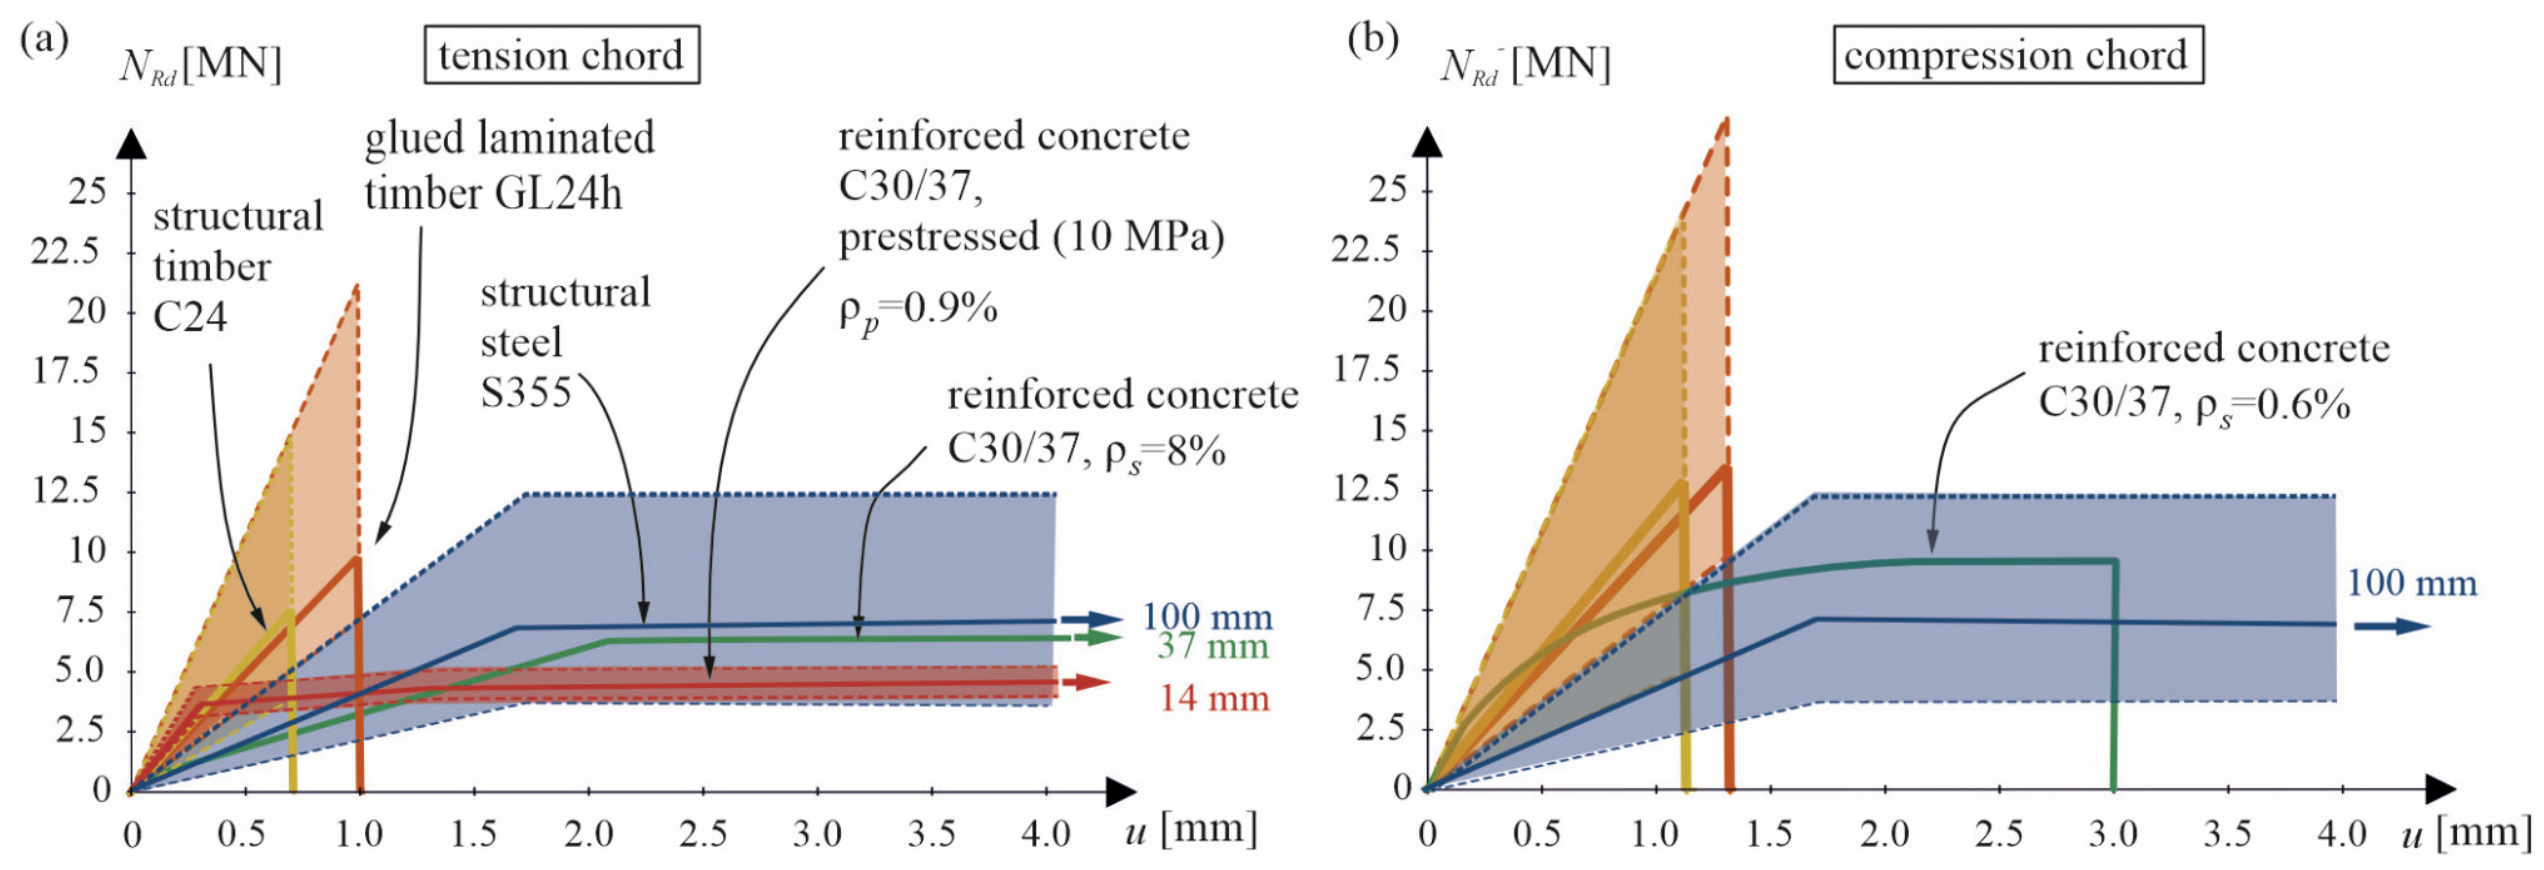
\includegraphics[width=0.9\textwidth]{IMAGES/LoadDeformationDiagram.png}
    \caption{Load-deformation diagrams of (a) tension and (b) compression members using structural timber, steel and reinforced (prestressed) concrete with a consumption of $100\ kg CO_{2}eq$ per running metre \cite{kfmResearch2026}.}
    \label{fig:LDdiagrams}
\end{figure}

A material with a higher initial embodied carbon per kilogram may prove more ecologically efficient if its superior mechanical capacity permits a significant reduction in the total volume of material required for the structure. However, this efficiency heavily depends on what becomes the governing design criterion. For example, the use of high-strength concrete has a considerably greater impact on strength than on stiffness, meaning the ecological benefit varies depending on the governing limit state.  Thus, over-designed elements must be avoided to ensure that the inherent mechanical capacity of the material is fully utilised.

\subsubsection{Efficiency of cross section}
The structural efficiency of a member is defined not only by the material used, but also by the geometric distribution of its cross section. Placing the same amount of material further away from the neutral axis increases the bending stiffness quadratically, according to Steiner’s theorem. Unfortunately, for slab structures, a flat ceiling is often desired to accommodate building services and to minimise overall storey height. Furthermore, complex cross sections are frequently more expensive to construct. In the past, material-efficient geometries, such as ribbed slabs, were the standard because material costs were relatively high compared to labour costs. This economic dynamic has since inverted, promoting the use of simpler but more material-intensive cross sections, such as solid rectangular concrete profiles \cite{Kaufmann2024_WhitePaper}.

\subsubsection{Efficiency of structural system}
The structural efficiency of a slab system is mainly influenced by the span of the system, whether it spans in one or multiple directions, and the continuity over the support. To illustrate this: A two-way spanning slab with continuity exhibits only one-tenth of the deflections compared to a one-way simply supported system, enabling much slender cross-sections. Whether continuity is achievable depends heavily on the chosen materialisation, as further elaborated in Section \ref{Sec: FloorSyst}. Furthermore, the span length largely influences the governing design criteria, with internal bending moments scaling proportionally to the span squared and deflections scaling proportionally to the span to the fourth power. Consequently, designers must strike a careful balance between selecting shorter spans to maximise structural and material efficiency, and maintaining adequate spatial flexibility to ensure a long service life for the building \cite{Kaufmann2024_WhitePaper}.


\subsection{Indirect influences \label{Sec: IndirectInfl}}

The loading of a structure is governed by its use. However, designers should critically review and discuss the loading scenario. For example, heavy and thick earth cover or unnecessarily high live load assumptions should be avoided. Often, structures are designed for heavier load scenarios for flexibility in the future. Similarly, non-continous systems are used for easier deconstruction for circularity purposes.
Those upfront carbon investments should always be taken with caution and only where a different scenario of use is intended, as designing a more efficient structure tailored for current needs will yield a lower overall environmental footprint \cite{Kaufmann2024_WhitePaper}.

The design choices of the structural system also have indirect influences on the overall environmental performance of the building in consequence. First, the total height of the structure plays a critical role. Increasing the depth of the member directly increases the total facade area and insulation area and reduces the usable floor space within a given zoning envelope. Second, the total mass of the building governs the design of the foundation, as higher structural loads require more foundation material. Both factors also increase the horizontal load through wind and earthquake, resulting in more extensive lateral load-resisting systems \cite{Kaufmann2024_WhitePaper}.

\section{Social and economic considerations}
Sustainability is generally defined in terms of its ecological, social, and economic dimensions \cite{Ammann2024}. Thus, the ecological sustainability assessment of Section \ref{Sec: SustainabilityAss} must be extended to satisfy user comfort, construction cost, and productivity requirements. Beyond these aspects, there are further considerations, such as health-related aspects. However, these are assumed to be outside the scope of this thesis.

\subsection{Serviceability and comfort \label{Sec: ServAndComf}}
In addition to limiting deflections, floor systems must satisfy vibration requirements to ensure adequate user comfort. This aspect becomes particularly relevant for lightweight floor systems due to their comparatively low stiffness and mass. Furthermore, floor systems must fulfil acoustic requirements, including both airborne and impact sound insulation. Achieving sufficient acoustic performance may require additional floor build-ups or increased structural mass. Consequently, lightweight floor systems often require additional measures to satisfy vibration and acoustic requirements, partially offsetting their ecological advantages \cite{BauphysikKalender}.

Particularly in Switzerland, these requirements are stringent and the expected level of comfort is high. Reducing these limits with respect to ecological sustainability is possible, but requires the client's approval \cite{Kaufmann2024_WhitePaper}. As these limits are very important for general health and public well-being, they should not be treated as soft constraints from the outset. However, assessing which criteria govern a specific floor system can help identify whether a discussion regarding comfort requirements in relation to ecological sustainability may be necessary.

\subsection{Importance of construction cost \label{Sec: ConstructionCost}}
The construction sector is a cost-driven environment, as competitive bidding is standard practice. Economically uncompetitive solutions will not to lead to widespread use. Therefore, for a practice-oriented comparison, the costs should also be taken into account to ensure financially feasible designs.

In advanced economies, labour cost is the most significant cost driver. Consequently, structurally or environmentally optimised systems are often not economically competitive. Ammann et al. \cite{Ammann2024} therefore state that “a conflict often arises between GWP and cost” when selecting a structural system. For this reason, the cost of a floor system is considered an important factor in the sustainability assessment.

\subsection{Construction productivity \label{Sec: Productivity}}
Compared to other industrial sectors, the construction industry has experienced only limited productivity improvements in recent decades \cite{Wangler2019}. As a result, improving construction productivity represents an important aspect of the future development of the construction industry.

In this context, prefabrication in combination with Building Information Modelling (BIM) offers significant potential to improve efficiency and reduce labour demand on-site \cite{Caulfield2022}. Furthermore, systems that enable faster construction progress, such as prefabricated timber elements or post-tensioned slabs with reduced propping times \cite{Rombach2010}, may help compensate for higher production costs or more complex geometries.

\section{Key factors that define sustainability}
The factors identified in the literature review serve as comparison criteria for evaluating the sustainability performance of floor systems. Sustainability is understood as comprising environmental, social, and economic dimensions. The assessment is carried out both for the structural slab alone and for the complete floor system, which includes the floor build-up required to meet acoustic insulation requirements.

\newcolumntype{L}[1]{>{\raggedright\arraybackslash}p{#1}}

\begin{table*}[h]
    \centering
    \begingroup
    \scriptsize
    \setlength{\tabcolsep}{4pt}
    \renewcommand{\arraystretch}{1.2}
    \begin{tabularx}{\textwidth}{@{}L{2.8cm}|L{3.6cm}|L{1.6cm}|X@{}}
    \hline
    \textbf{Name} &
    \textbf{Parameter} &
    \textbf{Unit} &
    \textbf{Reason} \\ \hline

    Global Warming Potential &
    $GWP_{\mathrm{struct}}$, $GWP_{\mathrm{tot}}$ &
    kg CO$_2$-eq/m$^2$ &
    Section \ref{Sec: SustainabilityAss}: GWP of the cross-section for its specific structural system while accounting for producer-specific material variations.  \\

    Height &
    $h_{\mathrm{struct}}$, $h_{\mathrm{tot}}$ &
    m &
    Section \ref{Sec: IndirectInfl}: Indirect influence total height.  \\

    Mass &
    $m_{\mathrm{struct}}$, $m_{\mathrm{tot}}$ &
    kN/m$^2$ &
    Section \ref{Sec: IndirectInfl}: Indirect influence total mass.  \\

    Cost &
    $cost_{\mathrm{struct}}$, $cost_{\mathrm{tot}}$ &
    CHF/m$^2$ &
    Section \ref{Sec: ConstructionCost}: Economic sustainability and market competitiveness\\

    Construction time &
    $T_{\mathrm{struct}}$, $T_{\mathrm{tot}}$ &
    h/m$^2$ &
    Section \ref{Sec: Productivity}: Productivity  \\ \hline
    \end{tabularx}
    \endgroup
    \caption{Sustainability factors for slab comparison. \label{Tab: SustFact}}
\end{table*}

\begin{table*}[h]
    \centering
    \begingroup
    \scriptsize
    \setlength{\tabcolsep}{4pt}
    \renewcommand{\arraystretch}{1.2}
    \begin{tabularx}{\textwidth}{@{}L{2.8cm}|L{5.0cm}|X@{}}
    \hline
    \textbf{Requirement} &
    \textbf{Limit} &
    \textbf{Verification in the slab configurator} \\ \hline

    ULS &
    $q_{k,\mathrm{zul,GZT}} \geq q_k$ &
    Ultimate limit state verification of bending and shear resistance under design load combinations \cite{SIA260_2013, SIA261_2020}. \\

    SLS 1 &
    $w_{\mathrm{install}} \leq L/350$
    
    $w_{\mathrm{use}} \leq L/350$
    
    $w_{\mathrm{app}} \leq L/300$ &
    Serviceability limit state verification of deflections, including installation, use and appearance deflection limits \cite{SIA260_2013, SIA261_2020}. \\

    SLS 2 &
    $f_1 \geq f_{1,\min}$, $a_{\mathrm{ed}} \leq a_{\mathrm{lim}}$, $w_{f,\mathrm{ed}} \leq w_{f,\mathrm{lim}}$, $v_{\mathrm{ed}} \leq v_{\mathrm{cd}}$ &
    Serviceability limit state verification of vibration behaviour, including natural frequency and vibration response checks \cite{Lignum3.1:2015, Ziegler2008Grundlagen}. \\

    Fire &
    $R_{\mathrm{fire}} \geq 60\,\mathrm{min}$ &
    Fire resistance verification according to the section-specific fire exposure and material rules \cite{SIA260_2013}. \\

        Acoustic requirements &
    Normal (Increased): $R_w \geq 53\,(57)\,\mathrm{dB}+\Delta_{\mathrm{plan}}$
    $L_{n,w} \leq 51\,(47)\,\mathrm{dB}-\Delta_{\mathrm{plan}}$
    
    $\Delta_{\mathrm{plan}}=5\,\mathrm{dB}$ for concrete
    $\Delta_{\mathrm{plan}}=8\,\mathrm{dB}$ for timber &
    Automated generation of the floor build-up to fulfil the selected acoustic requirement level, including airborne and impact sound checks \cite{SIA181_2020}. \\ \hline
    \end{tabularx}
    \endgroup
    \caption{Requirements according to the Swiss national standard that are fulfilled by the slab configurator.}
    \label{tab:configurator_requirements}
    \label{Tab: ReqSS}
\end{table*}

\section{Major types of floor systems\label{Sec: FloorSyst}}
For the purposes of this comparison, the floor systems most commonly used in building construction are identified and supplemented by more advanced alternatives that promise improved sustainability performance. Residential and office buildings represent the application area. Although the floor systems considered are used internationally, the review is tailored to the Swiss construction market. Furthermore, economic considerations, such as the comparatively high labour costs, are based on Swiss market conditions. In doing so, this section focuses on the broader system level. More refined modelling assumptions and considerations are introduced in Chapter \ref{sec:MM}.

Steel-concrete composite floor systems are not considered in this study, as they have historically seen limited application in Switzerland \cite{Mensinger2010}. Furthermore, digitally fabricated slabs and highly structurally optimised solutions are excluded, as they are not yet considered ready for widespread adoption in building practice and remain insufficiently covered by current design standards and regulations \cite{Wangler2019, Ranaudo2021HiLo}.



\subsection{Solid reinforced concrete slab}
The solid reinforced concrete slab is the current industry standard in Switzerland \cite{Ammann2024}. Local construction companies possess the necessary formwork systems, supports and the expertise gained through decades of practice, making this system economically competitive. Due to its geometric simplicity, flexibility for building service installations, inherent fire resistance and acoustic insulation, planners typically favour this system. Structurally, it relies on an efficient two-way load-bearing mechanism with continuity over the supports. However, in terms of cross-sectional performance, the flat slab is inefficient from a sustainability perspective. A significant portion of the concrete in the tension zone does not contribute to the structural capacity but adds considerable self-weight and embodied carbon.

\subsection{Ribbed reinforced concrete slab}
Ribbed slabs optimise material usage by concentrating concrete in the compression zone and utilising ribs in the tension zone to house the reinforcement. As a result, the self-weight is reduced, allowing for longer spans. However, the improved structural efficiency leads to an increased construction height and potentially reduced functionality of the floor system. The more refined cross-section requires complex formwork and a higher amount of manual labour, increasing costs especially in countries with high labour costs \cite{Ammann2024, Kaufmann2024_WhitePaper}.

\subsection{Post-tensioned solid concrete slab}
Looking at the current market situation, there is no denying that the advantages of a solid slab are important. Reduced overall height, spatial flexibility, unobstructed installation of building services, combined with the lowest cost per square metre of slab \cite{Ammann2024}. Thus, post-tensioned solid concrete slabs with unbonded tendons were included in the investigation as a system that combines the advantages of an inefficient solid slab with the structural efficiency provided by prestressing. \cite{Rombach2010}

Post-tensioned slabs introduce active compressive stresses into the concrete through high-strength steel tendons. As a result, post-tensioned slabs stay longer in the uncracked state, showing higher bending stiffnesses. Depending on the tendon trajectory, deviation forces can compensate part of the applied load. The degree of post-tensioning determines the extent to which the loads are balanced. \cite{Rombach2010, flachdecken_Morgen} 
Both effects improve serviceability behaviour with respect to deflections and enable longer spans or reduced slab thicknesses compared with conventional reinforced concrete slabs. Consequently, in the context of sustainability-optimised floor systems, post-tensioned slabs represent a major competitor, as they can reduce the required quantities of concrete and reinforcing steel while simultaneously minimising the overall building height.

For point supports, the punching behaviour is improved. The applied action is reduced by tendon deviation forces, while the resistance is increased through reduced slab rotations.

Post-tensioning solid slabs through unbonded tendons is not a new system. Early tendon layouts for two-way post-tensioned slabs, developed in the 1950s in the United States, typically consisted of uniformly distributed tendons with additional tendons in the support strips \cite{PTI2023}. However, these layouts increased the complexity of future slab penetrations \cite{Rombach2010}. Dual-banded layouts address this limitation and further improve the existing system. Here, the tendons are concentrated within the support strips above the columns. Advantageously, dual-banded prestressing leaves the central regions of the slab largely free of tendons, allowing penetrations and openings to be added with minimal risk of damaging tendons. In addition, the concentration of tendons along the column strips simplifies tendon installation, reduces coordination conflicts with other building services, and improves the practicality of slab optimisations in the span region, such as voided or waffle slab constructions \cite{PTI2023}.

\begin{figure}[htbp]
    \centering
    \resizebox{\textwidth}{!}{%
        \definecolor{tendonblue}{HTML}{1F4E99}

\begin{tikzpicture}[
    slab/.style={black, thick},
    tendon/.style={tendonblue, thin},
    gridline/.style={gray!45, dashed, thin},
    support/.style={draw, fill=gray!30, minimum size=0.28cm, inner sep=0pt},
    dim/.style={<->, thin},
    tick/.style={thin},
    txt/.style={font=\scriptsize},
    subtit/.style={font=\scriptsize\bfseries},
    note/.style={font=\scriptsize, align=center}
]

% Dimensions
\def\W{6.0}
\def\H{6.0}
\def\bayX{2.0}
\def\bayY{2.0}
\def\xA{0}
\def\xB{8.0}
\def\y{0}

% ============================================================
% (a) Distributed layout
% ============================================================

% Slab outline
\draw[slab] (\xA,\y) rectangle ++(\W,\H);

% Column grid lines
\foreach \xx in {0,2,4,6} {
    \draw[gridline] (\xA+\xx,\y-0.15) -- (\xA+\xx,\y+\H+0.15);
}
\foreach \yy in {0,2,4,6} {
    \draw[gridline] (\xA-0.15,\y+\yy) -- (\xA+\W+0.15,\y+\yy);
}

% Supports
\foreach \xx in {0,2,4,6} {
    \foreach \yy in {0,2,4,6} {
        \node[support] at (\xA+\xx,\y+\yy) {};
    }
}

% Distributed tendons aligned with column grid and extending to slab edges
\foreach \xx in {0,0.5,1.0,1.5,2.0,2.5,3.0,3.5,4.0,4.5,5.0,5.5,6.0} {
    \draw[tendon] (\xA+\xx,\y) -- (\xA+\xx,\y+\H);
}
\foreach \yy in {0,0.5,1.0,1.5,2.0,2.5,3.0,3.5,4.0,4.5,5.0,5.5,6.0} {
    \draw[tendon] (\xA,\y+\yy) -- (\xA+\W,\y+\yy);
}

% Dimensions x
\foreach \xx in {0,2,4} {
    \draw[dim] (\xA+\xx,\y+\H+0.45) -- (\xA+\xx+2,\y+\H+0.45);
    \draw[tick] (\xA+\xx,\y+\H+0.30) -- (\xA+\xx,\y+\H+0.60);
    \draw[tick] (\xA+\xx+2,\y+\H+0.30) -- (\xA+\xx+2,\y+\H+0.60);
    \node[txt] at (\xA+\xx+1,\y+\H+0.72) {$l_x$};
}

% Dimensions y
\foreach \yy in {0,2,4} {
    \draw[dim] (\xA+\W+0.45,\y+\yy) -- (\xA+\W+0.45,\y+\yy+2);
    \draw[tick] (\xA+\W+0.30,\y+\yy) -- (\xA+\W+0.60,\y+\yy);
    \draw[tick] (\xA+\W+0.30,\y+\yy+2) -- (\xA+\W+0.60,\y+\yy+2);
    \node[txt] at (\xA+\W+0.75,\y+\yy+1) {$l_y$};
}

% ============================================================
% (b) Banded layout
% ============================================================

% Slab outline
\draw[slab] (\xB,\y) rectangle ++(\W,\H);

% Column grid lines
\foreach \xx in {0,2,4,6} {
    \draw[gridline] (\xB+\xx,\y-0.15) -- (\xB+\xx,\y+\H+0.15);
}
\foreach \yy in {0,2,4,6} {
    \draw[gridline] (\xB-0.15,\y+\yy) -- (\xB+\W+0.15,\y+\yy);
}

% Supports
\foreach \xx in {0,2,4,6} {
    \foreach \yy in {0,2,4,6} {
        \node[support] at (\xB+\xx,\y+\yy) {};
    }
}

% Banded tendons along column strips, extending to slab edges
\foreach \yy in {0,2,4,6} {
    \foreach \dy in {-0.18,-0.09,0,0.09,0.18} {
        \draw[tendon] (\xB,\y+\yy+\dy) -- (\xB+\W,\y+\yy+\dy);
    }
}

\foreach \xx in {0,2,4,6} {
    \foreach \dx in {-0.18,-0.09,0,0.09,0.18} {
        \draw[tendon] (\xB+\xx+\dx,\y) -- (\xB+\xx+\dx,\y+\H);
    }
}

% Dimensions x with xi notation
\draw[dim] (\xB,\y+\H+0.45) -- (\xB+2,\y+\H+0.45);
\node[txt] at (\xB+1,\y+\H+0.72) {$l_x$};

\draw[dim] (\xB+2,\y+\H+0.45) -- (\xB+2.35,\y+\H+0.45);
\node[txt] at (\xB+2.175,\y+\H+0.72) {$\xi l_x$};

\draw[dim] (\xB+2.35,\y+\H+0.45) -- (\xB+3.65,\y+\H+0.45);
\node[txt] at (\xB+3.0,\y+\H+0.72) {$(1-2\xi)l_x$};

\draw[dim] (\xB+3.65,\y+\H+0.45) -- (\xB+4.0,\y+\H+0.45);
\node[txt] at (\xB+3.825,\y+\H+0.72) {$\xi l_x$};

\draw[dim] (\xB+4,\y+\H+0.45) -- (\xB+6,\y+\H+0.45);
\node[txt] at (\xB+5,\y+\H+0.72) {$l_x$};

\foreach \xx in {0,2,2.35,3.65,4,6} {
    \draw[tick] (\xB+\xx,\y+\H+0.30) -- (\xB+\xx,\y+\H+0.60);
}

% Dimensions y
\foreach \yy in {0,2,4} {
    \draw[dim] (\xB+\W+0.45,\y+\yy) -- (\xB+\W+0.45,\y+\yy+2);
    \draw[tick] (\xB+\W+0.30,\y+\yy) -- (\xB+\W+0.60,\y+\yy);
    \draw[tick] (\xB+\W+0.30,\y+\yy+2) -- (\xB+\W+0.60,\y+\yy+2);
    \node[txt] at (\xB+\W+0.75,\y+\yy+1) {$l_y$};
}

% Installation / optimisation field
\fill[magenta!25, draw=magenta!25, solid, thick]
    (\xB+4.2,\y+0.2) rectangle ++(1.6,1.6);
\node[note, magenta!90!black, font=\tiny] at (\xB+5,\y+0.70)
    {Installation /\\Optimisation};
\end{tikzpicture}%
}
    }
    \caption{Comparison of (a) distributed and (b) banded layouts for two-way post-tensioned slabs.}
    \label{fig:distributed_banded_tendon_layouts}
\end{figure}


\subsection{Solid timber slab}
Timber as a material offers a higher strength-to-weight ratio with a lower environmental impact than steel, making it an attractive structural material \cite{Wimmers2017}. Solid timber systems, primarily utilising glulam or cross-laminated timber elements, offer a high degree of prefabrication.
Due to the modular nature of timber construction, achieving continuity over supports is often challenging, resulting in the widespread use of simply supported systems. Furthermore, timber structures are generally designed elastically, as the brittle tensile failure of wood limits the potential for plastic redistribution. In contrast, reinforced concrete and steel structures are better suited for the development of hyperstatic continuous structural systems, in which internal force redistribution allows for increased bearing capacity.

Although wood is a combustible material, its fire behaviour can be predicted reliably, making its application feasible provided that a rigorous fire design is implemented \cite{frangi2008fire}. However, due to the comparatively low stiffness and mass of timber structures, timber slabs are frequently governed by serviceability limit states, particularly vibration and deflection criteria, rather than ultimate strength. In addition, the low mass of timber results in comparatively poor acoustic insulation, often requiring heavy and costly floor build-ups to meet regulatory requirements \cite{Kaufmann2024_WhitePaper}.


\subsection{Ribbed and hollow-core timber slabs}
These systems, such as timber ribs with a top (and bottom) plate, aim to increase the moment of inertia while maintaining the lightweight benefits of wood. Hollow cores are often used for acoustic insulation or integration of building services \cite{Frangi2009_HC}. Compared to mass timber, hollow-core systems are more complex to fabricate and often incorporate a variety of different materials, which can negatively affect their circularity and ease of deconstruction. However, hollow-core systems are typically delivered as prefabricated elements, enabling rapid construction progress on-site.

\subsection{Timber-concrete composite slabs}
These composite slabs combine the strengths of two distinct materials. Concrete is placed in the upper compression zone to provide stiffness, fire protection, and acoustic mass, while timber is used in the lower tension zone. Consequently, less reinforcement and concrete are required compared to a conventional reinforced concrete system, while acoustic insulation and fire protection are ensured by the concrete topping \cite{proHolz2012_Zuschnitt45}. The degree of composite action is governed by the stiffness of the shear connection between the two materials \cite{Eurocode5_2023}.

As with pure timber systems, timber-concrete composite systems lack complete continuity over the supports. Promisingly, there is sustained effort to enable at least partial continuity in the case of in-situ concrete \cite{durchlauf_HBV}. This is addressed in upcoming standards through the calculation of a single-span system with a reduced effective span \cite{Eurocode5_2023}.

\subsubsection{Solid timber-concrete composite slabs}
A solid timber-concrete composite slab typically consists of a glulam, cross-laminated timber or solid timber deck with a concrete topping. This configuration is frequently used in residential buildings, as structural and acoustic requirements can be met while maintaining a relatively slim profile. In such cases, notches in the timber panel are typically used as shear connectors \cite{proHolz2012_Zuschnitt45, Eurocode5_2023}.

\subsubsection{Ribbed timber-concrete composite slabs}
The ribbed timber-concrete composite slab uses solid timber- or glulam beams acting compositely with a thin concrete flange. This material-efficient composite system is capable of achieving longer spans with a very low self-weight-to-stiffness ratio. Here, screws, bonded steel rods, or steel plates are typically used as shear connectors \cite{proHolz2012_Zuschnitt45}.


\section{Quantify sustainability}
The three commonly acknowledged dimensions of sustainability are environmental, social and
economic sustainability \cite{Ammann2024}


\newpage
\chapter{Methods}\label{sec:MM}
\markright{\thechapter~Materials and methods}

\section{Slab configurator}
The computational work presented in this thesis is based on a Python-based design and optimisation framework initiated by the Sustainability in Structural Design Team at kfmResearch \cite{kfmResearch2026}. The original framework provided the general structure for the GWP optimisation of floor system cross-sections across different structural systems and for their environmental performance assessment. Within the scope of this thesis, the framework was further developed by incorporating additional slab systems and implementing the automated handling of non-structural floor build-ups.

The overall workflow is shown schematically in Figure~\ref{fig:slab_configurator_workflow}. The calculation starts with the material and product database. Based on the selected slab system, a cross-section object is created from the available materials and geometric start values. The cross-section is then combined with a member object, which defines the structural system, span, loading and requirements. The member is verified in ULS, SLS 1, SLS 2 and fire according to Table~\ref{Tab: SustFact}. For the structural cross-section a floor build-up is automatically created to satisfy the acoustic insulation requirements against airborne and impact sound. If the selected cross-section does not satisfy the governing requirements, the optimiser modifies selected cross-section parameters until a suitable design is found.  

\begin{figure}[htbp]
\centering
\resizebox{\textwidth}{!}{%
\begin{tikzpicture}[
    font=\scriptsize,
    >=Latex,
    arrow/.style={->, thick},
    note/.style={align=left},
    line/.style={thick}
]

% ------------------------------------------------------------------
% Column x-positions
% ------------------------------------------------------------------
\def\xData{0}
\def\xCS{4.2}
\def\xMember{10.8}

% Titles
\node[font=\bfseries\small] at (\xData,3.6) {Data};
\node[font=\bfseries\small] at (\xCS,3.6) {Cross-section};
\node[font=\bfseries\small] at (\xMember,3.6) {Member};

% ------------------------------------------------------------------
% Data block
% ------------------------------------------------------------------
\node[cylinder, draw, shape border rotate=90, aspect=0.25,
      minimum height=2.0cm, minimum width=1.25cm, align=center] (db) at (\xData,2.1)
      {Materials\\[2pt]CO$_2$ eq/m$^3$\\[2pt]CHF/m$^3$};

\node[note, anchor=north] at (\xData,0.85) {Material\\variations};

% ------------------------------------------------------------------
% Cross-section block
% ------------------------------------------------------------------
\coordinate (cs0) at (3.0,1.85);

\draw[line] (cs0) rectangle ++(2.8,0.85);
\fill[brown!80] ($(cs0)+(0,0)$) rectangle ++(2.8,0.35);
\fill[gray!60] ($(cs0)+(0,0.35)$) rectangle ++(2.8,0.30);
\fill[violet!70] ($(cs0)+(0,0.65)$) rectangle ++(2.8,0.08);
\fill[gray!30] ($(cs0)+(0,0.73)$) rectangle ++(2.8,0.12);

\draw[decorate,decoration={brace,amplitude=4pt}]
    (5.95,2.70) -- (5.95,2.50);

\node[anchor=west,align=left]
    at (6.15,2.80)
    {Automated\\[-4pt]floor build-up};

% Structural cross-section brace
\draw[decorate,decoration={brace,amplitude=4pt}]
    (5.95,2.50) -- (5.95,1.85)
    node[midway,right=6pt]
    {Cross-section};

\node[green!60!black, font=\large] at (8.25,2.1) {$\circlearrowleft$};
%\node[yellow!80!black, font=\large] at (8.15,3) {$\lightning$};

\node[note, anchor=north west] at (3.0,1.35) {Cross-section\\
$\bullet$ Fulfils requirements\\
$\bullet$ Optimised for GWP};

\node[green!60!black, font=\large] at (6.25,0.05) {$\circlearrowleft$};

% ------------------------------------------------------------------
% Member block
% ------------------------------------------------------------------
\coordinate (b1) at (10.0,2.10);
\coordinate (b2) at (12.3,2.10);

% Beam
\draw[line] (b1) -- (b2);

% Distributed load
\draw[red, thick] ($(b1)+(0,0.55)$) -- ($(b2)+(0,0.55)$);
\draw[red, thick] ($(b1)+(0,0.55)$) -- (b1);
\draw[red, thick] ($(b2)+(0,0.55)$) -- (b2);

\foreach \x in {10.0,10.75,11.50,12.3} {
    \draw[red, ->] (\x,2.65) -- (\x,2.25);
}

% Supports
\draw[line] (10.0,2.10) -- ++(-0.16,-0.27) -- ++(0.32,0) -- cycle;
\draw[line] (12.3,2.10) -- ++(-0.16,-0.27) -- ++(0.32,0) -- cycle;

% Span
%\draw[<->] (10.0,1.45) -- (12.3,1.45);
%\node at (11.15,1.22) {$L$};

% Member labels
\node[note, anchor=west] at (12.65,2.55) {Load combination};
\node[note, anchor=west] at (12.65,1.85) {Structural system};

\node[note, anchor=north west] at (10.0,1.35) {Requirements\\
$\bullet$ ULS\\
$\bullet$ SLS 1: Deflection\\
$\bullet$ SLS 2: Vibration\\
$\bullet$ Fire};

% ------------------------------------------------------------------
% Arrows between blocks
% ------------------------------------------------------------------
\draw[arrow] (1.25,2.1) -- (2.25,2.1);
\draw[arrow] (8.55,2.1) -- (9.45,2.1);

\end{tikzpicture}%
}
\caption{Slab configurator workflow from material database to cross-section optimisation and member comparison.}
\label{fig:slab_configurator_workflow}
\end{figure}

The comparison is carried out in two stages. First, each slab system is optimised for the selected design criterion and span. Second, the resulting feasible members are compared according to the identified factors for sustainability, defined in Table~\ref{Tab: SustFact}.

It is noted that the slab configurator is used as a comparative design tool. It does not replace a detailed project-specific structural design, but it enables a consistent assessment of the relative influence of slab system, span, material choice, acoustic build-up and governing design criterion.


\subsection{Material database}
The material database was selected by the Sustainability in Structural Design Team of \textit{kfmResearch} \cite{kfmResearch2026}. It contains mechanical material properties and product-specific environmental data. Environmental Product Declarations (EPDs) are stored on product level and are linked to the mechanical property classes used by the structural models. The database therefore allows a distinction between mechanical performance and producer-specific environmental impact. For concrete, reinforcing steel, prestressing steel, and timber products, the database stores product density, material class and total GWP values. These properties enable the assessment of producer-specific GWP, mass, and structural height, including product-specific variations. As identified in the literature review, GWP, mass, and height are key indicators for the sustainability assessment of floor systems.

The range of product-specific GWP values stored in the database is summarised in Table~\ref{tab:product_specific_gwp_values}. Negative values occur for timber products where biogenic carbon storage is included in the reported GWP. Each product is assigned to a material class, which defines the corresponding mechanical and physical properties listed in Table~\ref{tab:material_properties}.

\begin{table*}[h]
    \centering
    \begingroup
    \scriptsize
    \setlength{\tabcolsep}{3pt}
    \renewcommand{\arraystretch}{1.12}
    \begin{tabularx}{\textwidth}{@{}
        >{\raggedright\arraybackslash}X
        |>{\raggedright\arraybackslash}X
        |c|r|r@{}}
    \hline
    \textbf{Material} &
    \textbf{Material class} &
    \textbf{Products} &
    \textbf{$GWP_{\min}$} &
    \textbf{$GWP_{\max}$} \\
    &
    &
    &
    kg CO$_2$-eq/t &
    kg CO$_2$-eq/t \\
    \hline

    Ready-mixed concrete & C20/25 & 7  & 77.0   & 102.4 \\
    Ready-mixed concrete & C25/30 & 8  & 75.4   & 100.1 \\
    Ready-mixed concrete & C30/37 & 9  & 76.7   & 104.2 \\
    Reinforcing steel    & B500B  & 18 & 352.9  & 922.7 \\
    Prestressing steel   & Y1860  & 9  & 389.0  & 2250.0 \\
    Glue-laminated timber& GL24h  & 21 & -1534.9& 765.5 \\
    Solid structural timber & C24 & 10 & 75.7   & 363.0 \\
    3- and 5-ply wood    & C24    & 13 & -66.2  & 556.0 \\
    3- and 5-ply wood    & GL24h  & 3  & 250.0  & 415.6 \\
    \hline
    \end{tabularx}
    \endgroup
    \caption{Product-specific GWP values used for the sustainability assessment.}
    \label{tab:product_specific_gwp_values}
\end{table*}

\begin{table*}[htbp]
    \centering
    \begingroup
    \scriptsize
    \setlength{\tabcolsep}{3pt}
    \renewcommand{\arraystretch}{1.15}
    \begin{tabularx}{\textwidth}{@{}>{\raggedright\arraybackslash}X|r|r|r|r|r|r|r|r|>{\raggedright\arraybackslash}X|r|r@{}}
    \hline
    \textbf{Class} &
    \textbf{$f_c$} &
    \textbf{$f_t$} &
    \textbf{$f_m$} &
    \textbf{$f_v$} &
    \textbf{$E$} &
    \textbf{$\rho$} &
    \textbf{$\beta_n$} &
    \textbf{$\varphi$} &
    \textbf{Connector type} &
    \textbf{$d$} &
    \textbf{$K_{\mathrm{ser}}$} \\
    &
    MPa &
    MPa &
    MPa &
    MPa &
    GPa &
    kg/m$^3$ &
    mm/min &
    -- &
    -- &
    mm &
    N/m \\
    \hline

    C20/25 &
    20 &
    2.3 &
    -- &
    -- &
    30 &
    2241–2440 &
    -- &
    2.5 &
    -- &
    -- &
    -- \\

    C25/30 &
    25 &
    2.6 &
    -- &
    -- &
    32 &
    2242–2439 &
    -- &
    2.5 &
    -- &
    -- &
    -- \\

    C30/37 &
    30 &
    2.9 &
    -- &
    -- &
    34 &
    2332–2430 &
    -- &
    2.5 &
    -- &
    -- &
    -- \\

    B500B &
    500 &
    500 &
    -- &
    -- &
    205 &
    7850 &
    -- &
    -- &
    -- &
    -- &
    -- \\

    GL24h &
    -- &
    -- &
    24 &
    1.8 &
    11.5 &
    424–483 &
    0.7 &
    0.6 &
    -- &
    -- &
    -- \\

    C16 &
    -- &
    -- &
    16 &
    1.5 &
    8.0 &
    500 &
    0.8 &
    0.6 &
    -- &
    -- &
    -- \\

    C24 &
    -- &
    -- &
    24 &
    1.5 &
    11.0 &
    400–523 &
    0.8 &
    0.6 &
    -- &
    -- &
    -- \\

    Y1860 &
    -- &
    1860 &
    -- &
    -- &
    195 &
    7850 &
    -- &
    -- &
    -- &
    -- &
    -- \\

    DBS\_6 &
    -- &
    -- &
    -- &
    -- &
    -- &
    -- &
    -- &
    -- &
    Screw &
    6 &
    $5.83 \times 10^6$ \\

    DBS\_8 &
    -- &
    -- &
    -- &
    -- &
    -- &
    -- &
    -- &
    -- &
    Screw &
    8 &
    $7.78 \times 10^6$ \\

    DBS\_10 &
    -- &
    -- &
    -- &
    -- &
    -- &
    -- &
    -- &
    -- &
    Screw &
    10 &
    $9.70 \times 10^6$ \\

    DBS\_12 &
    -- &
    -- &
    -- &
    -- &
    -- &
    -- &
    -- &
    -- &
    Screw &
    12 &
    $1.167 \times 10^7$ \\

    Kerve\_20 &
    -- &
    -- &
    -- &
    -- &
    -- &
    -- &
    -- &
    -- &
    Notched &
    -- &
    $1.00 \times 10^9$ \\

    Kerve\_30 &
    -- &
    -- &
    -- &
    -- &
    -- &
    -- &
    -- &
    -- &
    Notched &
    -- &
    $1.50 \times 10^9$ \\

    Two-layer parquet &
    -- &
    -- &
    -- &
    -- &
    -- &
    555 &
    -- &
    -- &
    -- &
    -- &
    -- \\

    Cement screed &
    -- &
    -- &
    -- &
    -- &
    21.0 &
    1850 &
    -- &
    -- &
    -- &
    -- &
    -- \\

    Insulation (glass wool) &
    -- &
    -- &
    -- &
    -- &
    $6\times10^{-6}$ &
    80 &
    -- &
    -- &
    -- &
    -- &
    -- \\
    
    Crushed gravel &
    -- &
    -- &
    -- &
    -- &
    -- &
    2000 &
    -- &
    -- &
    -- &
    -- &
    -- \\

    \hline
    \end{tabularx}
    \endgroup
    \caption{Mechanical properties data on characteristic design level. Mass is stored producer-specific.}
    \label{tab:material_properties}
\end{table*}

During the thesis, the database was extended with material-specific (not producer-specific) cost and construction time as listed in Table~\ref{tab:cost_time_assumptions}. The values are derived from NPK positions, market data, literature sources and engineering estimates.

\begin{table*}[htbp]
    \centering
    \begingroup
    \scriptsize
    \setlength{\tabcolsep}{3pt}
    \renewcommand{\arraystretch}{1.12}
    \begin{tabularx}{\textwidth}{@{}X|c|c|c|c|X@{}}
    \hline
    \textbf{Material / Component} &
    \textbf{Cost} &
    \textbf{Cost unit} &
    \textbf{Time} &
    \textbf{Time unit} &
    \textbf{Reference and description} \\ \hline

    Ready-mixed concrete, formwork &
    75.71 & CHF/m$^2$ & 0.70 & h/m$^2$ &
    NPK 241.261.301, logistics, propping, levelling, oiling and cleaning \cite{CIB19076}.\\

    Ready-mixed concrete, rib. formwork &
    151.42 & CHF/m$^2$ & 1.40 & h/m$^2$ &
    Logistics, propping, levelling, oiling and cleaning \cite{Ammann2024}.\\

    Reinforcing steel &
    2.01 & CHF/kg & 0.009 & h/kg &
    NPK 241.511.123, placing \cite{CIB19076}.\\

    Prestressing steel &
    6.00 & CHF/kg & 0.020 & h/kg &
    Assumed cost and labour input. \\

    Ready-mixed concrete &
    205.29 & CHF/m$^3$ & 0.30 & h/m$^3$ &
    NPK 241.661.112, placing, vibrating, levelling and cleaning \cite{CIB19076}. \\

    Glue-laminated timber &
    1750.00 & CHF/m$^3$ & 1.00 & h/m$^3$ &
    Assumed market price including logistics and connections. \\

    Solid structural timber &
    1250.00 & CHF/m$^3$ & 1.00 & h/m$^3$ &
    NPK 335.531.114, logistics and connections. \\

    DBS 6, Screw TCC conn., d=6 mm &
    5.00 & CHF/piece & 0.010 & h/piece &
    Assumed, logistics and assembly. \\

    DBS 8, Screw TCC conn., d=8 mm &
    5.50 & CHF/piece & 0.010 & h/piece &
    Assumed, logistics and assembly. \\

    DBS 10, Screw TCC conn., d=10 mm &
    6.00 & CHF/piece & 0.015 & h/piece &
    Assumed, logistics and assembly. \\

    DBS 12, Screw TCC conn., d=12 mm &
    6.50 & CHF/piece & 0.015 & h/piece &
    Assumed, logistics and assembly. \\

    Kerve, TCC connector &
    30.00 & CHF/piece & 0.010 & h/piece &
    Assumed, preparation and cleaning. \\

    Two-layer parquet, 11 mm &
    106.00 & CHF/m$^2$ & 0.30 & h/m$^2$ &
    Swiss market price according to \cite{Bodenleger2026}. \\

    Cement screed &
    337.60 & CHF/m$^3$ & 0.15 & h/m$^2$ &
    NPK 661.711.111, labour productivity according to \cite{Steelmonks2026}. \\

    Insulation (glass wool) &
    335.00 & CHF/m$^3$ & 0.10 & h/m$^2$ &
    NPK 661.433.114, acoustic insulation layer. \\

    Crushed gravel &
    253.20 & CHF/m$^3$ & 0.20 & h/m$^2$ &
    NPK 364.921.111, ballast and protection layer. \\ \hline
    \end{tabularx}
    \endgroup
    \caption{Cost and construction-time input data used for the sustainability assessment.}
    \label{tab:cost_time_assumptions}
\end{table*}

\newpage
\subsection{Contribution to the existing Python framework}
Since this thesis is based on an existing Python framework, it is important to highlight the contributions made within its scope. The initial configurator was able to handle solid rectangular concrete, ribbed concrete, solid rectangular timber, and ribbed timber hollow-core cross-sections. The one-dimensional static systems covered were simple-span and continuous beams. For the two-dimensional case, the framework was able to handle line-supported rectangular slabs without continuity over the supports.

\subsubsection{Cross-section handling}
All cross-section classes were updated with respect to the calculation of material quantities, GWP, cost, and construction time. These calculations are now normalised per square metre of floor area and account for quantities that develop in the transverse direction. This enables a consistent comparison between one-dimensional systems with defined tributary widths and two-dimensional slab systems.
Furthermore, all systems were linked to the automated acoustic floor build-up generator described in Section~\ref{Sec: AutFloor}. Following the structural optimisation, the generator determines the lightest floor build-up that satisfies the specified acoustic requirements.
The specific modifications made to the individual cross-section classes are summarised in Table~\ref{tab:existing_system_developments}.

\begin{table*}[h]
    \centering
    \begingroup
    \scriptsize
    \setlength{\tabcolsep}{3pt}
    \renewcommand{\arraystretch}{1.15}
    \begin{tabularx}{\textwidth}{@{}
        >{\raggedright\arraybackslash}p{3.2cm}
        |>{\raggedright\arraybackslash}X
        |>{\raggedright\arraybackslash}X@{}}
    \hline
    \textbf{Cross-section class} &
    \textbf{Further development} &
    \textbf{Effect on the assessment} \\
    \hline

    Ribbed timber hollow-core &
    Internal cavity insulation added to the acoustic model and non-structural mass calculation. &
    Improves the acoustic model of the hollow-core cross-section.\\

    Ribbed reinforced concrete &
    Separate resistance checks introduced for positive span bending and negative support bending.  &
    Extends ULS validation from span moment to support moment.  \\

    Rectangular reinforced concrete &
    Two-way slab analysis extended to include upper support reinforcement in the optimisation for continuous systems. As equal spans are assumed, the optimised reinforcement in the \(x\)-direction is applied in the \(y\)-direction. &
    Enables the optimisation of negative bending reinforcement quantities for continuous systems. \\

    Point-supported reinforced concrete &
    Punching shear calculation of the required punching reinforcement resistance. Required punching reinforcement is converted into an additional steel quantity. &
    Includes the environmental, economic and construction-time effects of punching reinforcement without excluding systems solely based on the need for such reinforcement. \\

    \hline
    \end{tabularx}
    \endgroup
    \caption{Cross-section-specific developments introduced for existing structural systems.}
    \label{tab:existing_system_developments}
\end{table*}

\subsubsection{Static system handling}
The analysis of two-dimensional floor systems was extended to distinguish between line-supported and point-supported structural systems. In addition, continuity over the supports was introduced. Internal forces and deflections were determined in accordance with the existing implementation using:

\begin{equation}
\begin{aligned}
M_d &= \alpha_{M,\mathrm{system}} q_d l^2,\\
V_d &= \alpha_{V,\mathrm{system}} q_d l,\\
w &= \alpha_{w,\mathrm{system}}\frac{q_d l^4}{EI}.
\end{aligned}
\end{equation}

The coefficients $\alpha_{M,\mathrm{system}}$, $\alpha_{V,\mathrm{system}}$, and $\alpha_{w,\mathrm{system}}$ were derived from a finite-element slab analysis performed in Cubus Cedrus. For point-supported systems, the model consisted of a regular $4 \times 4$ column grid subjected to a uniformly distributed load. The columns had a cross-section of $0.25 \times 0.25 \mathrm{m}$. Line-supported systems were represented by walls with a thickness of $0.20\mathrm{m}$ and a height of $0.10\mathrm{m}$. Vertical displacements at the supports were restrained. Bending moments and shear forces were evaluated over an averaged width of one metre within the support strip, whereas deflections were evaluated at mid-span. The coefficients were determined for spans of 3, 5, 6, 7, 8, 10, 12, and 16\,m and subsequently implemented in the configurator through a database storage.

For ULS bending verification of two-dimensional rectangular concrete slabs, plastic moment redistribution was added as an optional modification of the elastic moment coefficients. The elastic coefficients from the slab database remain the basis for the analysis, but they are replaced by redistributed coefficients when the slab system and the cross-section provide sufficient rotational capacity. This redistribution is only applied to reinforced and post-tensioned rectangular concrete slabs. The available ductility classes of the positive and negative bending zones are compared with the required ductility classes stored for the corresponding slab system. If the requirement is not fulfilled, the elastic coefficients are retained. If it is fulfilled, positive span moments are increased and negative support moments are reduced by system-specific factors:

\begin{equation}
\alpha_{M,\mathrm{red},i}
=
\begin{cases}
k_{+}\,\alpha_{M,i}, & \alpha_{M,i} \geq 0,\\
k_{-}\,\alpha_{M,i}, & \alpha_{M,i} < 0.
\end{cases}
\end{equation}

For line-supported continuous slabs, the factors \(k_{+}=1.51\) and \(k_{-}=0.76\) were used. For point-supported continuous slabs, the factors were \(k_{+}=1.47\) and \(k_{-}=0.68\). The redistributed moment coefficients are used only in the ULS bending resistance check; shear, punching shear, deflection and vibration checks remain based on the corresponding elastic coefficients.

\subsection{Timber--concrete composite slab}

Timber--concrete composite (TCC) slabs were modelled as unidirectional structural systems consisting of a timber tension member and a concrete compression layer. Composite action is partially achieved through mechanical shear connectors. Inclined screw connectors were used for ribbed systems, while notched connections were used for flat timber plate systems.

\subsubsection{$\gamma$-method}

The implemented model for partial shear connection follows the $\gamma$-method according to EN 1995-1-1 \cite{Eurocode5_2023}. The effective bending stiffness is calculated as
\begin{equation}
(EI)_{\mathrm{ef}}
=
\sum_{i=1}^{2}
\left(
E_i I_i
+
\gamma_i E_i A_i a_i^2
\right),
\qquad
\gamma_1
=
\left(
1+
\frac{\pi^2 E_1 A_1 s_1}{K l^2}
\right)^{-1},
\qquad
\gamma_2 = 1.
\end{equation}
Index 1 refers to the concrete layer and index 2 to the timber layer. The factors $\gamma_i$ describe the efficiency of the composite action resulting from the finite slip stiffness of the connection. The distances from the composite neutral axis to the centroids of the concrete and timber components, as well as the connector stiffness, are calculated as
\begin{equation}
\begin{aligned}
a_1
&=
\frac{h_1+h_2}{2}
+d
-a_2,
\\
a_2
&=
\frac{
\gamma_1 E_1 A_1
\left(
\frac{h_1+h_2}{2}
+
d
\right)
}
{
\gamma_1 E_1 A_1
+
\gamma_2 E_2 A_2
},
\\
K
&=
\frac{2}{3}K_{\mathrm{ser}}.
\end{aligned}
\end{equation}
For the concrete compression flange, an effective width is considered according to
\begin{equation}
\begin{aligned}
b_{\mathrm{ef}}
&=
b_{\mathrm{ef},1}
+
b_{\mathrm{ef},2}
+
b_w,
\\
b_{\mathrm{ef},i}
&=
\min
\left(
0.2\,b_i
+
0.1\,l_0,
\;
0.2\,l_0
\right).
\end{aligned}
\end{equation}
Here, $E_i$, $I_i$ and $A_i$ are the modulus of elasticity, second moment of area and cross-sectional area of part $i$, respectively. The connector spacing is denoted by $s_1$, while $K$ is the connector slip modulus used in the $\gamma$-method. Furthermore, $l_0$ is the span length, $b_i$ is the width of part $i$, $b$ is the distance between ribs, $h_i$ is the depth of part $i$, and $d$ is the depth of the formwork or interlayer.

\subsubsection{Time-dependent behaviour}

TCC systems are verified at different time states because stresses redistribute between timber and concrete due to their different time-dependent creep behaviour. For the ULS of the composite cross-section, the quasi-permanent design load and the short-term component are calculated as
\begin{equation}
\begin{aligned}
q_{\mathrm{perm},d}
&=
1.25
\left(
\gamma_G\, g_{k,\mathrm{tot}}
+
\psi_{01}\,\gamma_Q\, q_{k1}
\right),
\\
q_{\mathrm{short},d}
&=
(1-\psi_{01})
\,\gamma_Q\, q_{k1}.
\end{aligned}
\end{equation}
For the SLS, the permanent, frequent and rare load combinations are calculated as
\begin{equation}
\begin{aligned}
q_{\mathrm{perm}}
&=
g_{k,\mathrm{tot}}
+
\psi_{21}\,q_{k1},
\\
q_{\mathrm{freq}}
&=
g_{k,\mathrm{tot}}
+
\psi_{11}\,q_{k1},
\\
q_{\mathrm{rare}}
&=
g_{k,\mathrm{tot}}
+
q_{k1}.
\end{aligned}
\end{equation}
The verification for the intermediate period of 3--7 years, which accounts for differential shrinkage, is not required as the ULS check is verified for 125\% of the quasi-permanent load \cite{CENTS191032021}. The calculations consider the concrete creep coefficient $\varphi$, the timber deformation factor $k_{\mathrm{def}}$ and the effective connector deformation factor
\begin{equation}
k'_{\mathrm{def}}
=
2k_{\mathrm{def}}.
\end{equation}
Consequently, ULS verification is separated into short-term and quasi-permanent loading situations, each using different effective stiffnesses. SLS verifications also account for long-term effects. For deflection calculations, a distinction is made between short-term and quasi-permanent loading, whereas vibration calculations are based on the stiffness at $t=0$ and assume an uncracked concrete section in the transverse direction. In accordance with CEN/TS 19103 \cite{CENTS191032021}, the effective bending stiffnesses $EI_{\mathrm{ULS},t=0}$, $EI_{\mathrm{ULS},t=\infty}$, $EI_{\mathrm{SLS},t=0}$ and $EI_{\mathrm{SLS},t=\infty}$ were calculated accordingly.

\subsubsection{Resistance verification}

The moment and shear resistances are determined per metre width of slab. The governing bending resistance is obtained from the minimum reserve of the concrete compression zone and the timber bending resistance. Figure \ref{fig:composite_section} illustrates the stress distribution assumed for the verification.

\begin{figure}[H]
    \centering
    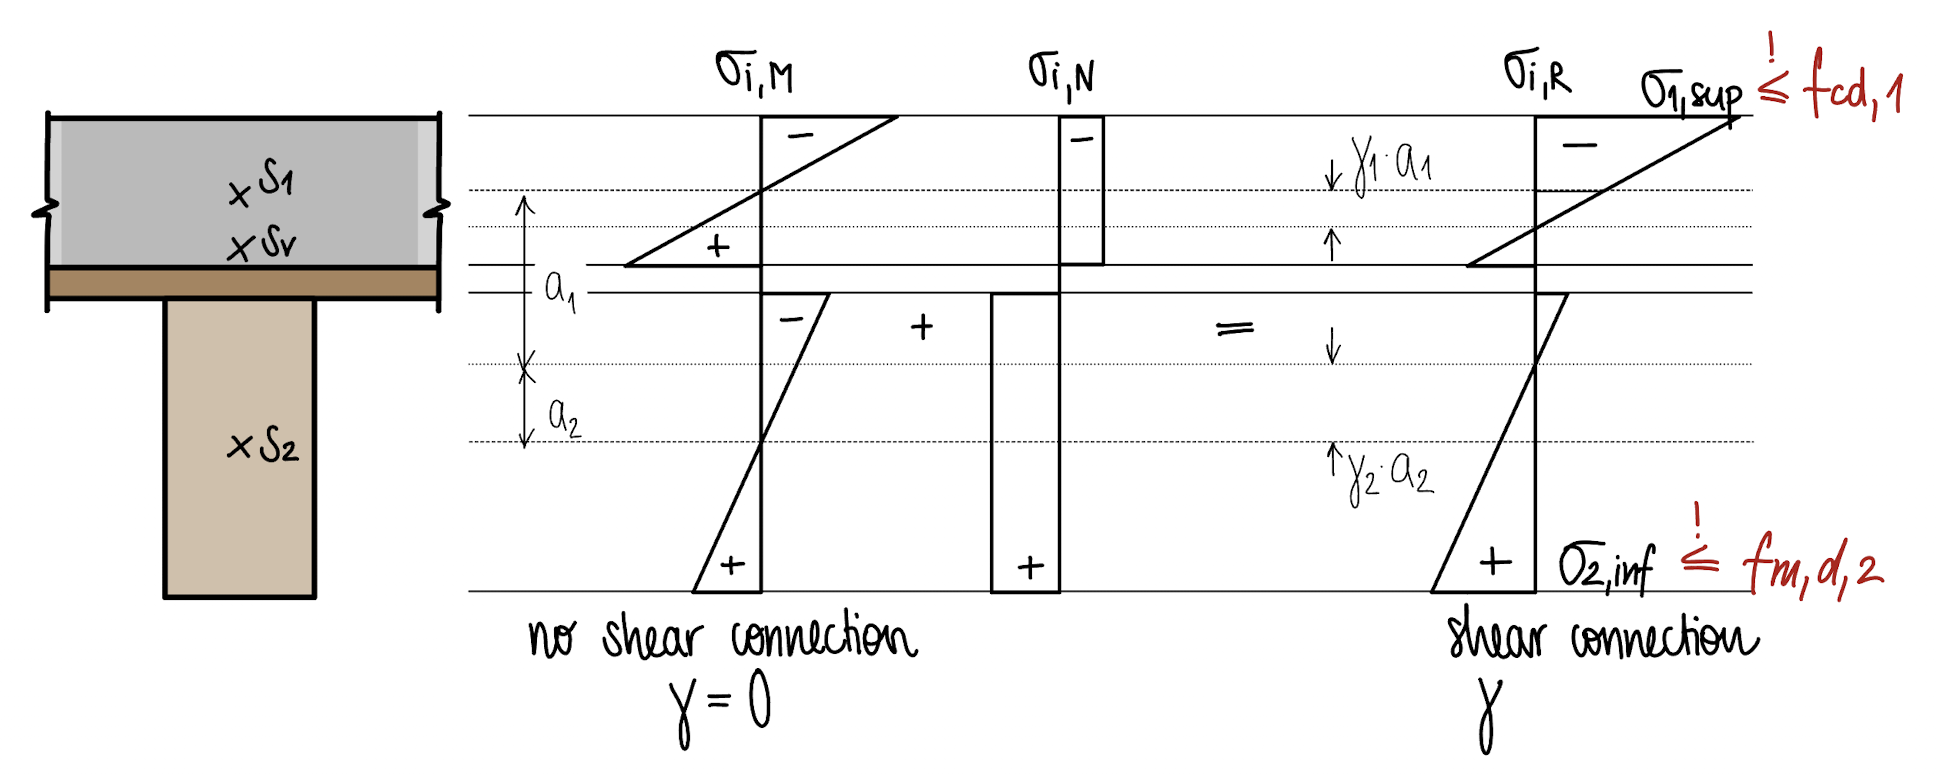
\includegraphics[width=0.9\textwidth]{IMAGES/CS_sigmas.png}
    \caption{Cross-section of a two-layer composite beam with semi-rigid connection according to EN 1995-1-1 \cite{Eurocode5_2023}.}
    \label{fig:composite_section}
\end{figure}

The bending and shear resistances are calculated as
\begin{equation}
\begin{aligned}
m_u
&=
\frac{1}{b}
\min
\left(
f_{cd,1}
\frac{(EI)_{\mathrm{ef}}}{E_1}
\frac{1}{\gamma_1 a_1 + h_1/2},
\;
f_{md,2}
k_{\mathrm{mod}}
\frac{(EI)_{\mathrm{ef}}}{E_2}
\frac{1}{a_2 + h_2/2}
\right),
\\
v_u
&=
\frac{
2 f_{vd,2} k_{\mathrm{mod}}
}
{b}
\frac{(EI)_{\mathrm{ef}}}{E_2}
\frac{1}
     {(a_2+h_2/2)^2}.
\end{aligned}
\end{equation}
The shear resistance is governed by the timber member. For simplification, the shear connection was assumed to be sufficient. Consequently, the detailed design of the connectors was not considered and no connector resistance verification was performed.

\subsubsection{Fire verification}

Fire resistance was evaluated using the residual timber cross-section after charring. A distinction was made between beams exposed on three sides and timber plates exposed on one side. For notched connections, no temperature-dependent reduction in connector stiffness was considered. For screw connectors, the reduction factor $k_{\mathrm{mod,fi}}$ according to Lignum 3.1 was applied \cite{Lignum3.1:2015}.

To satisfy the REI60 requirement, a minimum concrete topping thickness of 80 mm was required \cite{SIA262_2025}. Furthermore, a timber cover of 30 mm was reserved for screw connectors to account for the arrangement of two screws placed side by side.

\subsubsection{Model limitations}

Several simplifications were adopted. The model is limited to one-way structural behaviour and linear-elastic composite action according to the $\gamma$-method. Concrete is assumed to remain uncracked. The shear connection was assumed to provide sufficient resistance. Furthermore, non-linear connector behaviour and differential shrinkage between timber and concrete were not considered.

\subsection{Post-tensioned concrete slab}

Post-tensioned concrete slabs were modelled as flat concrete slabs with unbonded monostrands \cite{Rombach2010, flachdecken_Morgen}. The model extends the reinforced concrete slab formulation by prestressing steel, tendon geometry, load-balancing effects, secondary internal forces, effective bending stiffness, and the additional shear and punching shear resistance provided by tendon deviation forces. The implemented system assumes parabolic tendon profiles. For one-dimensional systems, a distributed tendon layout was assumed. For two-dimensional systems, tendon layouts were represented by distributed and/or banded tendon arrangements, depending on the selected layout configuration.

\subsubsection{Load balancing and tendon geometry}

The post-tensioning force was determined from the load-balancing principle. For a parabolic tendon trajectory, the upward deviation load depends on the prestressing force, tendon eccentricity and span length. For distributed tendons, the equivalent deviation loads in the two orthogonal directions are calculated as

\begin{equation}
u_x
=
\frac{8p_x f_x}{l_x^2},
\qquad
u_y
=
\frac{8p_y f_y}{l_y^2}.
\end{equation}

Here, \(p_x\) and \(p_y\) are the distributed prestressing forces per metre width, \(f_x\) and \(f_y\) are the tendon sag values, and \(l_x\) and \(l_y\) are the corresponding spans. The implemented load-balancing algorithm assigns the required balanced load depending on the selected tendon layout. For distributed tendons in both directions, the structural self-weight is split equally between the two directions and represented by equivalent surface deviation loads. For banded layouts, the tendons are concentrated in the support strips and the internal forces caused by prestressing are derived from equivalent line loads acting along these strips. The prestressing force is selected to balance the structural self-weight estimate available during tendon layout generation.

The tendon profile was defined by the support and mid-span eccentricities. For a parabolic profile,

\begin{equation}
z(x)
=
-\frac{4(e_{\mathrm{span}}-e_{\mathrm{sup}})}{l^2}\,x^2
+
\frac{4(e_{\mathrm{span}}-e_{\mathrm{sup}})}{l}\,x
+
e_{\mathrm{sup}}.
\end{equation}

The eccentricities were selected as the maximum values that satisfy the tendon cover, avoid overlap with the bonded reinforcement and remain within the slab depth. The tendon input values were \(A_p=150\,\mathrm{mm^2}\), \(c_{p,\mathrm{nom}}=30\,\mathrm{mm}\) and \(r_p=6.91\,\mathrm{mm}\).

\subsubsection{Secondary internal forces}

In hyperstatic systems, the deformation caused by post-tensioning is restrained by the supports. This restraint introduces secondary bending moments and secondary shear forces. The total internal forces resulting from the deviation forces of the prestressing system are first calculated using the slab-system coefficients. The secondary internal forces are then obtained by subtracting the primary prestressing contribution:

\begin{equation}
M_{\mathrm{sec}}
=
M_{\mathrm{tot}}(u)
-
P\,e,
\qquad
V_{\mathrm{sec}}
=
V_{\mathrm{tot}}(u)
-
P\,\frac{\partial e}{\partial x}.
\end{equation}

Here, \(M_{\mathrm{tot}}\) and \(V_{\mathrm{tot}}\) denote the total internal forces of the hyperstatic system caused by the deviation forces, \(P\) is the prestressing force and \(e\) is the tendon eccentricity. These secondary internal forces are included in the resistance verification of the post-tensioned slab.

\subsubsection{Effective bending stiffness}

Post-tensioning introduces compressive stresses into the concrete and therefore delays cracking under service loads. For SLS verification, the effective bending stiffness is determined based on the relation between the acting service moment, including secondary moments, and the cracking moment. The cracking moment, initial concrete stress and effective tensile strength are calculated as

\begin{equation}
\begin{aligned}
M_R
&=
\left(
f_{\mathrm{ctm,eff}}
-
\sigma_{c,\mathrm{inf},0}
\right)
\frac{I_I}{h/2},\\
\sigma_{c,\mathrm{inf},0}
&=
-\frac{P}{l\,h}
-
\frac{P\,e_{\max}\,h}{2l\,I_I},\\
f_{\mathrm{ctm,eff}}
&=
\max
\left[
(1.6-h)\,f_{\mathrm{ctm}},
\;
f_{\mathrm{ctm}}
\right].
\end{aligned}
\end{equation}

If the acting service moment does not exceed the cracking moment, the uncracked stiffness is used:

\begin{equation}
(EI)_{\mathrm{eff}}
=
E_{cm}I_I
\qquad
\text{for}
\qquad
\left|M_{\mathrm{Ed,SLS}}+M_{\mathrm{sec}}\right|
\leq
M_R.
\end{equation}

If the cracking moment is exceeded, a partial-cracking factor is calculated and the effective stiffness is interpolated between the uncracked and cracked states as implemented in the code:

\begin{equation}
\begin{aligned}
\zeta
&=
1
-
0.5
\left(
\frac{M_R}{|M_{\mathrm{Ed,SLS}}+M_{\mathrm{sec}}|}
\right)^2,\\
(EI)_{\mathrm{eff}}
&=
\zeta (EI)_I
+
(1-\zeta)(EI)_{II}.
\end{aligned}
\end{equation}

For cracked sections, the local increase of the post-tensioning force is neglected because strain compatibility between concrete and unbonded tendons is not maintained. The cracked neutral-axis depth \(x_{II}\) is obtained from force and moment equilibrium using the effective prestressing force as an external normal force:

\begin{equation}
\begin{aligned}
A_s\sigma_s
+
\frac{P}{l}
&=
\frac{b\,x_{II}}{2}\sigma_{c,\mathrm{inf}},
\\
d_sA_s\sigma_s
+
d_P\frac{P}{l}
+
M_{\mathrm{Ed,SLS}}
+
M_{\mathrm{sec}}
&=
\frac{b\,x_{II}^2}{6}\sigma_{c,\mathrm{inf}}.
\end{aligned}
\end{equation}

The stresses are calculated as

\begin{equation}
\sigma_s
=
\frac{\varepsilon_{c,\mathrm{inf}}}{x_{II}}
(d_s-x_{II})E_s,
\qquad
\sigma_{c,\mathrm{inf}}
=
E_{cm}\varepsilon_{c,\mathrm{inf}}.
\end{equation}

The cracked bending stiffness is calculated from the concrete compression zone and the transformed bonded reinforcement contribution:

\begin{equation}
(EI)_{II}
=
E_{cm}
\left[
\frac{x_{II}^3}{3}
+
\frac{E_s}{E_{cm}}
A_s
(d_s-x_{II})^2
\right].
\end{equation}

The prestressing tendon is not added as a transformed reinforcement area in the cracked inertia because the tendon is unbonded and local strain compatibility is not assumed. Creep is considered in the member deflection calculation through the service load combinations and creep amplification, rather than by reducing \(E_{cm}\) directly in the cracked-section stiffness calculation in accordance with the existing rectangular concrete handling.

\subsubsection{Bending and one-way shear resistance}

The bending resistance accounts for the contribution of the prestressing steel and the bonded reinforcement. The design bending moment includes the effects of external loads and secondary moments:

\begin{equation}
M_d
=
M_{g,d}
+
M_{q,d}
+
M_{\mathrm{sec}}
\leq
M_{Rd}.
\end{equation}

The bending resistance and the corresponding compression-zone depth are calculated as

\begin{equation}
\begin{aligned}
M_{Rd}
&=
\frac{P}{l}
\left(
d_P-\frac{0.85x}{2}
\right)
+
A_s f_{sd}
\left(
d_s-\frac{0.85x}{2}
\right),
\\
x
&=
\frac{
A_s f_{sd}
+
P/l
}
{
b_{\mathrm{eff}} f_{cd}
}.
\end{aligned}
\end{equation}

Ductility is ensured by limiting the compression-zone depth and by providing minimum bonded reinforcement. For the minimum bonded reinforcement check, the ordinary reinforced-concrete cracking moment is used, while the prestress-increased cracking moment is used for serviceability stiffness.

For systems without column supports, one-way shear is checked. The design shear force includes the secondary shear force and is verified against the concrete shear resistance and the vertical component of the prestressing force:

\begin{equation}
\begin{aligned}
V_d
&=
V_{g,d}
+
V_{q,d}
+
V_{\mathrm{sec}}
\leq
V_{Rd}
+
P_{\infty}\sin(\beta_P),\\
\sin(\beta_P)
&=
\frac{4f}{L}.
\end{aligned}
\end{equation}

Here, \(V_{Rd}\) is calculated according to the reinforced concrete shear resistance model of the rectangular concrete section. The post-tensioning contribution is added through the vertical component of the prestressing force.

\subsubsection{Punching shear resistance}

For slabs supported by columns, punching shear is checked instead of one-way shear. The concrete punching resistance without punching reinforcement is implemented as level of approximation 2 \cite{SIA262_2025}:

\begin{equation}
\begin{aligned}
V_{Rd,c}(\psi)
&=
k_r\,\tau_{cd}\,d_v\,u,
\\
k_r
&=
\frac{1}
{
0.45
+
0.18\,\psi\,d_v\,k_g
}
\leq
2,
\qquad
k_g
=
\frac{48}
{16+D_{\max}}.
\end{aligned}
\end{equation}

The slab rotation is calculated as

\begin{equation}
\begin{aligned}
\psi
&=
1.5
\frac{r_s}{d_v}
\frac{f_{sd}}{E_s}
\left(
\frac{m_{sd}}{m_{Rd}}
\right)^{3/2},\\
r_s &= 0.22l.
\end{aligned}
\end{equation}

The rotation is determined independently for both orthogonal directions, and the larger value governs:

\begin{equation}
\psi
=
\max(\psi_x,\psi_y).
\end{equation}

The design action is calculated as

\begin{equation}
V_{Ed}
=
V_{g,d}
+
V_{q,d}
+
V_{\mathrm{sec}},
\end{equation}

where \(V_{\mathrm{sec}}\) is the secondary shear force caused by restraint of the prestressing deformation. Without punching reinforcement, the verification is

\begin{equation}
V_{Ed}
\leq
V_{Rd,c}(\psi).
\end{equation}

For post-tensioned slabs, the resistance is increased by the vertical component of the prestressing force above the column:

\begin{equation}
V_{Rd,\mathrm{punch}}
=
V_{Rd,c}(\psi)
+
V_{P,\mathrm{punch}}.
\end{equation}

The prestressing contribution is calculated from the support-strip tendons and the distributed tendons crossing the control width around the column:

\begin{equation}
V_{P,\mathrm{punch}}
=
\left(
P_{sx,\infty}
+
p_{dx,\infty} b_{0,y}
\right)
\sin(\beta_{P,x})
+
\left(
P_{sy,\infty}
+
p_{dy,\infty} b_{0,x}
\right)
\sin(\beta_{P,y}).
\end{equation}

The forces \(P_{sx}\) and \(P_{sy}\) are the post-tensioning forces in the support strips and are assumed to act fully over the column. Distributed tendons are only considered over the relevant control width around the column.

If punching reinforcement is required, the existing shear reinforcement definition of the cross-section is used for the resistance calculation. No separate punching reinforcement object is introduced in the structural model. For material accounting in the final comparison, required punching reinforcement is post-processed as an additional averaged steel quantity. The resistance is calculated as

\begin{equation}
V_{Rd,\mathrm{punch}}
=
V_{Rd,c}(\psi)
+
V_{Rd,s}
+
V_{P,\mathrm{punch}},
\end{equation}

with an upper limit applied to the sum of concrete and punching reinforcement resistance in the implementation.

\subsubsection{Model limitations}

Several simplifications were adopted. The model is limited to unbonded monostrands with parabolic tendon profiles. Friction losses were neglected. Local anchorage verification and local concrete crushing at anchorages were not considered. For cracked sections, the local increase in prestressing force is neglected because strain compatibility is not maintained for unbonded tendons. The model also assumes that the selected prestressing layout can be arranged within the geometric constraints of the slab and anchorage system. The effective stiffness model is a simplified post-processing approach and does not include a transformed unbonded tendon contribution in the cracked inertia.

\subsection{Automated acoustic floor build-up generator \label{Sec: AutFloor}}

The generator enables floor build-up handling dependent on the structural cross-section. It adds the lightest non-structural floor build-up that satisfies the selected airborne and impact sound targets. The purpose is to compare slab systems on the basis of complete floor assemblies rather than structural cross-sections only. The generator distinguishes between normal and increased acoustic requirements according to SIA 181 \cite{SIA181_2020}. The target values are summarised in Table~\ref{Tab: ReqSS}.

The workflow of the generator is shown in Figure~\ref{fig:acoustic_floor_generator}. First, the structural cross-section is converted into an area-related mass. Airborne sound insulation and impact sound level are then estimated with the mass-law relationship \cite{BauphysikKalender, ISO12354_1_2017, ISO12354_2_2017}:

\begin{equation}
\begin{aligned}
R_{w,\mathrm{mass}} &= 37.5 \log_{10}(m'_{\mathrm{base}}) - 42,\\
L_{n,w,\mathrm{mass}} &= 164 - 35 \log_{10}(m'_{\mathrm{base}}).
\end{aligned}
\end{equation}

If the bare structural cross-section does not fulfil the acoustic targets, a floating floor consisting of glass wool, cement screed and parquet is added. Screed thicknesses of 60 mm and 85 mm are checked first. The floating floor is represented by a simplified mass-spring-mass model \cite{BauphysikKalender, ISO12354_1_2017, ISO12354_2_2017}:

\begin{equation}
\begin{aligned}
(s'_{\mathrm{eff}})^{-1}
&=
\sum_i (s'_i)^{-1},\\
f_{0,R} &=
\frac{1}{2\pi}
\sqrt{
s'_{\mathrm{eff}}\,10^6
\left(
\frac{1}{m'_{\mathrm{base}}}
+
\frac{1}{m'_{\mathrm{screed}}}
\right)
},\\
\Delta R_{w,\mathrm{fl}} &=
74.4 - 20\log_{10}(f_{0,R}) - \frac{R_{w,\mathrm{mass}}}{2},\\
f_{0,L} &=
160\sqrt{\frac{s'_{\mathrm{eff}}}{m'_{\mathrm{screed}}}},\\
\Delta L_{n,w,\mathrm{fl}} &=
\operatorname{mean}_{f_i \leq f_{\max}}
\left[
30\log_{10}
\left(
\frac{f_i}{f_{0,L}}
\right)
\right].
\end{aligned}
\end{equation}

Here, \(s'_{\mathrm{eff}}\) is the effective dynamic stiffness of the glass-wool layer in \(\mathrm{MN/m^3}\). For TCC sections with two insulation layers, the layers are treated as springs in series.

If the acoustic targets are still not met, gravel is added below the spring layer in discrete steps. TCC sections use a separate branch because the concrete topping is already part of the structural cross-section. The concrete layer is therefore treated as mass and impact damping, and no additional gravel is generated. Gravel, hollow-core insulation and the TCC concrete topping all use damping corrections \cite{BauphysikKalender}.

\begin{figure}[htbp]
\centering
\resizebox{\textwidth}{!}{%
    \begin{tikzpicture}[
    font=\small,
    >=Latex,
    arrow/.style={->, thick},
    box/.style={draw, rounded corners=1pt, align=center, minimum width=3.2cm, minimum height=1.0cm},
    widebox/.style={draw, rounded corners=1pt, align=center, minimum width=4.4cm, minimum height=1.12cm},
    eqbox/.style={draw, rounded corners=1pt, align=center, minimum width=5.1cm, minimum height=1.35cm},
    corrbox/.style={draw, rounded corners=1pt, align=center, minimum width=6.1cm, minimum height=1.8cm}
]

\node[box] (section) at (0,0) {Structural\\cross-section};
\node[eqbox] (mass) at (4.7,0) {Mass law\\[-1pt]
    \(m'_{\mathrm{base}}\)\\[1pt]
    \(R_{w,\mathrm{mass}}, L_{n,w,\mathrm{mass}}\)};
\node[box] (checkbare) at (9.5,0) {Targets\\fulfilled?};
\node[box] (none) at (13.9,1.65) {No additional\\floor build-up};
\node[widebox] (floating) at (13.9,-1.65) {Floating floor\\glass wool + screed + parquet};
\node[eqbox] (spring) at (19.3,-1.65) {Mass-spring-mass\\[-1pt]
    \(f_{0,R}, f_{0,L}\)\\[1pt]
    \(\Delta R_{w,\mathrm{fl}},\Delta L_{n,w,\mathrm{fl}}\)};
\node[corrbox] (damping) at (25.4,-1.65) {Damping corrections\\[-1pt]
    gravel: \(\Delta_{\mathrm{gravel}}\leq6\,\mathrm{dB}\)\\[-1pt]
    hollow-core: \(\Delta_{\mathrm{hc}}=\min(6h_{\mathrm{ins}}/0.20,7)\)\\[-1pt]
    TCC topping: \(\Delta_{\mathrm{tcc}}\leq6\,\mathrm{dB}\)};
\node[widebox] (tcc) at (19.3,-3.75) {TCC branch\\topping as mass\\and impact damping};
\node[eqbox] (output) at (32.0,0) {Complete floor assembly\\[-1pt]
    \(R_w=R_{w,\mathrm{mass}}+\Delta R\)\\[1pt]
    \(L_{n,w}=L_{n,w,\mathrm{mass}}-\Delta L\)};

\draw[arrow] (section) -- (mass);
\draw[arrow] (mass) -- (checkbare);
\draw[arrow] (checkbare) -- node[above, font=\small] {yes} (none);
\draw[arrow] (checkbare) -- node[below, font=\small] {no} (floating);
\draw[arrow] (floating) -- (spring);
\draw[arrow] (spring) -- (damping);
\draw[arrow] (floating) -- (tcc);
\draw[arrow] (none) -| (output);
\draw[arrow] (damping) -| (output);
\draw[arrow] (tcc) -| (damping);

\end{tikzpicture}

}
\caption{Workflow of the automated acoustic floor build-up generator.}
\label{fig:acoustic_floor_generator}
\end{figure}

The implemented acoustic model is intentionally simplified. A fully spectral prediction would require measured $R(f)$, $L_n(f)$ and $\Delta L(f)$ data for every structural system and floor layer. Such data is not available consistently for all systems in the optimisation. Thus, the model averages across the calculated frequencies. The selected model is therefore used as a robust comparative approximation, not as a replacement for project-specific acoustic verification.

\subsection{Final comparison setup}

The final comparison was defined through a set of residential and office cases with fixed load levels, discrete span values, structural systems and material groups. The cases are summarised in Table~\ref{tab:final_comparison_cases}. The corresponding start values, optimisation variables and bounds are listed in Table~\ref{tab:final_comparison_bounds}. This separation keeps the comparison inputs transparent: Table~\ref{tab:final_comparison_cases} defines which systems are compared, while Table~\ref{tab:final_comparison_bounds} defines how each system is optimised.

\begin{table*}[t]
    \centering
    \begingroup
    \scriptsize
    \setlength{\tabcolsep}{3.5pt}
    \renewcommand{\arraystretch}{1.2}
    \begin{tabularx}{\textwidth}{@{}l|c|l|>{\hsize=0.7\hsize\raggedright\arraybackslash}X|>{\hsize=0.7\hsize\raggedright\arraybackslash}X|>{\hsize=0.8\hsize\raggedright\arraybackslash}X|>{\hsize=1.8\hsize\raggedright\arraybackslash}X@{}}
    \hline
    \textbf{Case} &
    \textbf{$q_k$} &
    \textbf{Span} &
    \textbf{Cross-section} &
    \textbf{Description} &
    \textbf{Structural system} &
    \textbf{Materials / fixed input} \\
    & kN/m$^2$ & m & & & & \\ \hline
    Residential & 2.0 & 3, 5, 6, 7, 8, 10 &
    Rectangular concrete &
    conventionally reinforced &
    2-way, full continuity, walls &
    ready-mixed concrete, B500B; fixed line supports \\

    Residential & 2.0 & 3, 5, 6, 7, 8, 10 &
    Rectangular concrete PT &
    post-tensioned, distributed layout &
    2-way, full continuity, walls &
    ready-mixed concrete, B500B, Y1860; layout $[0,1,0,1]$; fixed line supports\\

    Residential & 2.0 & 3, 5, 6, 7, 8, 10 &
    Rectangular wood &
    BSH &
    Simple span &
    glue-laminated timber and solid structural timber; fire from bottom \\

    Residential & 2.0 & 3, 5, 6, 7, 8, 10 &
    TCC &
    BSH, kerve, $s=0.50$\,m &
    Simple span &
    ready-mixed concrete, B500B, BSH, kerve; $a_{\mathrm{ribs}}=1.00$\,m, $b_w=1.00$\,m \\

    Residential & 2.0 & 3, 5, 6, 7, 8, 10 &
    TCC &
    ribs, DBS\_10, $s=0.06$\,m (2 rows $s=0.12$\,m) &
    Simple span &
    ready-mixed concrete, B500B, BSH, DBS\_10; $a_{\mathrm{ribs}}=0.625$\,m, $b_w=0.18$\,m \\

    Residential & 2.0 & 3, 5, 6, 7, 8, 10 &
    Ribbed timber &
    hollow-core &
    Simple span &
    glue-laminated timber and solid structural timber; fire from bottom and sides \\

    Office & 3.0 & 8, 10, 12, 16 &
    Rectangular concrete &
    conventionally reinforced &
    2-way, full continuity, columns &
    ready-mixed concrete, B500B; fixed point supports \\

    Office & 3.0 & 8, 10, 12, 16 &
    Rectangular concrete PT &
    post-tensioned, distributed layout &
    2-way, full continuity, columns &
    ready-mixed concrete, B500B, Y1860; layout $[0,1,0,1]$; fixed point supports \\

    Office & 3.0 & 8, 10, 12, 16 &
    Rectangular concrete PT &
    post-tensioned, banded layout &
    2-way, full continuity, columns &
    ready-mixed concrete, B500B, Y1860; layout $[1,0,1,0]$; fixed point supports \\

    Office & 3.0 & 8, 10, 12, 16 &
    Ribbed concrete &
    conventionally reinforced &
    Continuous beam &
    ready-mixed concrete, B500B; fire from bottom and sides \\

    \hline
    \end{tabularx}
    \endgroup
    \caption{Input definition for the final comparison of slab systems. Only the discrete span values available in \texttt{slab\_properties.db} are used. The listed material groups are taken from \texttt{database\_260126.db}; for each mechanical property, the dataset generator considers the best and worst available EPD by GWP.}
    \label{tab:final_comparison_cases}
\end{table*}

\begin{table*}[t]
    \centering
    \begingroup
    \scriptsize
    \setlength{\tabcolsep}{4pt}
    \renewcommand{\arraystretch}{1.2}
    \begin{tabularx}{\textwidth}{@{}l|>{\hsize=0.7\hsize\raggedright\arraybackslash}X|l|>{\hsize=1.3\hsize\raggedright\arraybackslash}X@{}}
    \hline
    \textbf{Cross-section} &
    \textbf{Start values} &
    \textbf{Optimisation variables} &
    \textbf{Bounds / fixed values} \\ \hline

    Rectangular concrete 2D &
    $b=1.00$\,m, $h=0.20$\,m generally; office start heights $h_0=\{0.25,0.35,0.45,0.60\}$\,m for $l=\{8,10,12,16\}$\,m &
    $h$, $\varnothing_{xu}$, $\varnothing_{xo}$, $\varnothing_w$ &
    $h=0.16$--$1.20$\,m, $\varnothing_{xu/xo}=6$--$40$\,mm, $\varnothing_w=0$--$20$\,mm; $s=0.15$\,m; y-reinforcement follows x-reinforcement \\

    Rectangular concrete PT 2D &
    $b=1.00$\,m, $h=0.20$\,m generally; office start heights $h_0=\{0.20,0.25,0.30,0.40\}$\,m for $l=\{8,10,12,16\}$\,m &
    $h$, $\varnothing_{xu}$, $\varnothing_{xo}$, $\varnothing_w$ &
    $h=0.18$--$1.20$\,m, $\varnothing_{xu/xo}=6$--$40$\,mm, $\varnothing_w=0$--$20$\,mm; $s=0.15$\,m; Y1860 monostrands; load balancing from PT layout \\

    Rectangular wood 1D &
    $b=1.00$\,m, $h=0.10$\,m &
    $h$ &
    section height optimised for the governing criterion; glue-laminated timber and solid structural timber variations from database \\

    Ribbed timber 1D &
    $b=0.12$\,m, $h=0.22$\,m, $a=0.625$\,m, $t_2=25$\,mm, $t_3=27$\,mm &
    $b$, $h$, $t_2$, $t_3$ &
    $b=0.10$--$0.24$\,m, $h=0.22$--$2.00$\,m, $t_2=25$--$160$\,mm, $t_3=27$--$160$\,mm; rib spacing fixed at $a=0.625$\,m \\

    Ribbed concrete 1D &
    $b=1.00$\,m, $b_w=0.25$\,m, $h=0.30$\,m, $h_f=0.18$\,m &
    $h_w$, $h_f$, $\varnothing_{x,w}$, $b_w$, $b$ &
    $h_w=0.04$--$2.00$\,m, $h_f=0.08$--$0.50$\,m in 1D / $0.12$--$0.50$\,m in 2D optimiser, $\varnothing_{x,w}=8$--$40$\,mm, $b_w=0.15$--$0.40$\,m, $b=0.40$--$2.50$\,m \\

    TCC 1D &
    Residential: $h_c=0.08$\,m, $h_w=0.12$\,m; office TCC starts $(h_c/h_w)=0.12/0.30$, $0.16/0.35$, $0.20/0.40$, $0.25/0.70$\,m for $l=8$, 10, 12, 16\,m &
    $h_c$, $h_w$ &
    $h_c=0.08$--$0.50$\,m, $h_w=0.08$--$1.50$\,m; flat residential $s=0.50$\,m; ribbed residential $s=0.15$\,m, $b_w=0.18$\,m; ribbed office $s=0.06$\,m, $b_w=0.24$\,m \\ \hline
    \end{tabularx}
    \endgroup
    \caption{Start values, optimisation variables and bounds used for the final comparison. All systems are optimised for GWP with $n_{\mathrm{iter}}=150$; the automated acoustic floor build-up is enabled with normal acoustic requirements. Material variations are generated from the EPD best and worst cases within each mechanical property class.}
    \label{tab:final_comparison_bounds}
\end{table*}

\subsubsection{Sampling of material variants}

In the final comparison, material variation is generated by selecting the best and worst available EPD by GWP within each mechanical property group. Thus, for example, concrete strength class C30/37 is sampled with its lowest and highest available product-specific GWP, but it is not mixed with another strength class.

\subsection{Verification of implemented models}

\subsubsection{Timber--concrete composite slab}

The implementation of the $\gamma$-method was verified against a hand calculation based on a representative timber--concrete composite floor system. The selected geometry, material properties and connector configuration corresponded to a typical residential floor. The verification focused on the effective bending stiffness, as this quantity governs both resistance and serviceability calculations.

The verification model used the following set-up:

\begin{itemize}
    \item Concrete C30/37: $h_c = 0.080\,\mathrm{m}$, $b_{\mathrm{ef}} = 0.60\,\mathrm{m}$, $A_c = 0.048\,\mathrm{m}^2$, $I_c = 2.56 \times 10^{-5}\,\mathrm{m}^4$, $E_{cm} = 34\,\mathrm{GPa}$, $\varphi_c = 2.5$.
    
    \item Timber ribs GL24h: $a_{\mathrm{ribs}} = 0.6\,\mathrm{m}$, $h_w = 0.241\,\mathrm{m}$, $b_w = 0.12\,\mathrm{m}$, $A_w = 0.0289\,\mathrm{m}^2$, $I_w = 1.399 \times 10^{-4}\,\mathrm{m}^4$, $E_{w,\mathrm{mean}} = 11.5\,\mathrm{GPa}$, $d = 0.02\,\mathrm{m}$, $k_{\mathrm{def}} = 0.6$.
    
    \item Connection DBS\_10: $s = 0.25\,\mathrm{m}$, $K_{\mathrm{ser}} = 9.7\,\mathrm{MN/m}$, $k'_{\mathrm{def}} = 1.2$.
    
    \item Structural system: single-span system with $l_0 = 6.0\,\mathrm{m}$.
\end{itemize}


Table~\ref{tab:TCCVer} summarises the calculated $\gamma_c$ factors, the lever arms to the neutral axis ($a_c$ and $a_w$), and the resulting effective bending stiffness per metre width. The comparison showed excellent agreement between the manual calculations and the implementation. The maximum deviation remained below $0.2\,\%$, confirming the correct implementation of the $\gamma$-method across the time-dependent stiffness calculations.

\begin{table}[h!]
    \centering
    \begingroup
    \scriptsize
    \setlength{\tabcolsep}{3pt}
    \renewcommand{\arraystretch}{1.12}
    \begin{tabularx}{\textwidth}{@{}l|c|c|c|c|r|r@{}}
    \hline
    \textbf{Case} &
    \textbf{Time} &
    $\gamma_c$ &
    $a_c$ [m] &
    $a_w$ [m] &
    $EI_{\mathrm{eff,manual}}$ [$\mathrm{kN\,m^2/m}$] &
    $EI_{\mathrm{eff,test}}$ [$\mathrm{kN\,m^2/m}$] \\
    \hline
    SLS & $t=0$       & 0.0798 & 0.1299 & 0.0508 & 9225.00 & 9238.66 \\
    SLS & $t=\infty$ & 0.2279 & 0.1459 & 0.0348 & 4053.00 & 4059.49 \\
    ULS & $t=0$       & 0.0547 & 0.1425 & 0.0382 & 7962.00 & 7972.65 \\
    ULS & $t=\infty$ & 0.1645 & 0.1541 & 0.0265 & 3537.00 & 3540.68 \\
    \hline
    \end{tabularx}
    \endgroup
    \caption{Comparison of manual calculations to test-case output for effective bending stiffness values in $\mathrm{kN\,m^2/m}$.}
    \label{tab:TCCVer}
\end{table}

\subsubsection{Post-tensioned concrete slab}

The implementation of the post-tensioned slab class was checked using a diagnostic test file with a fixed set-up. The verification case covers the bending resistance and the quasi-permanent deflection of a two-way post-tensioned slab with distributed tendons and wall supports.

The verification model used the following set-up:

\begin{itemize}
    \item Materials: concrete C30/37, reinforcing steel B500B, prestressing steel Y1860.
    \item Structural system: two-way slab with wall supports and \(l_x=l_y=6.0\,\mathrm{m}\).
    \item Geometry: slab thickness \(h=280\,\mathrm{mm}\), effective depth of bonded steel \(d_s\), and effective depth of prestressing steel \(d_P\) as calculated from the reinforcement and tendon cover constraints.
    \item Tendon layout: distributed
    \item Loads: \(g_{0,k}\), \(g_{2,k}=0.75\,\mathrm{kN/m^2}\), \(q_k=2.00\,\mathrm{kN/m^2}\),  \(\varphi=2.0\).
\end{itemize}

The bending resistance was calculated from the contribution of the prestressing steel and the bonded reinforcement:

\begin{equation}
    M_{Rd}
    =
    \frac{P_{\infty}}{l}
    \left(d_p-\frac{0.85x}{2}\right)
    +
    A_s f_{sd}
    \left(d_s-\frac{0.85x}{2}\right)
\end{equation}

\begin{equation}
\begin{aligned}
x
&=
\frac{\frac{P_{\infty}}{l}+A_s f_{sd}}
{b f_{cd}},\\
\frac{P_{\infty}}{l}
&=
76.39\,\mathrm{kN/m},\\
A_s
&=
\frac{\pi \cdot 14^2}{4 \cdot 150}
=
1026\,\mathrm{mm^2/m},\\
f_{sd} &= 435\,\mathrm{MPa},
\qquad
f_{pd}=1391\,\mathrm{MPa},\\
x &= 31.36\,\mathrm{mm},
\qquad
0.85x=26.65\,\mathrm{mm}.
\end{aligned}
\end{equation}

The prestressing and bonded reinforcement contributions are

\begin{equation}
\begin{aligned}
M_{Rd,p}
&=
76.39
\left(
0.2431-\frac{0.02665}{2}
\right)
=
17.55\,\mathrm{kNm/m},\\
M_{Rd,s}
&=
1026 \cdot 10^{-6}
\cdot 435000
\left(
0.253-\frac{0.02665}{2}
\right)
=
106.94\,\mathrm{kNm/m},\\
M_{Rd}
&=
17.55+106.94
=
124.49\,\mathrm{kNm/m}.
\end{aligned}
\end{equation}

\paragraph{Deflection calculation}

The quasi-permanent load combination, the net load after load balancing and the long-term reference deflection are

\begin{equation}
\begin{aligned}
q_{\mathrm{per}}
&=
g_{0,k}+g_{1,k}+g_{2,k}+\psi_2 q_k
=
7.00+0.00+0.75+0.30\cdot2.00
=
8.35\,\mathrm{kN/m^2},\\
g_{0,k}
&=
7.00\,\mathrm{kN/m^2},\\
q_{\mathrm{net}}
&=
q_{\mathrm{per}}-g_{0,k}
=
1.35\,\mathrm{kN/m^2}.
\end{aligned}
\end{equation}

In Cubus Cedrus the same action was applied with the corresponding sign convention. The uncracked elastic deflection and long-term deflection are

\begin{equation}
\begin{aligned}
q_{\mathrm{net,Cedrus}}
&=
-1.350\,\mathrm{kN/m^2},\\
w_{\mathrm{Cedrus},\varphi=0}
&=
0.0349\,\mathrm{mm},\\
w_{\varphi}
&=
w_{\varphi=0}(1+\varphi),\\
w_{\mathrm{Cedrus},\varphi=2.0}
&=
0.0349\cdot3
=
0.1047\,\mathrm{mm}.
\end{aligned}
\end{equation}


The hand calculation is compared with the output of \inlinecode{test\_pt\_2D.py}.

\begin{table}[H]
    \centering
    \begingroup
    \scriptsize
    \setlength{\tabcolsep}{3pt}
    \renewcommand{\arraystretch}{1.12}
    \begin{tabularx}{0.65\textwidth}{@{}l|r|r|r@{}}
    \hline
    \textbf{Result} & \textbf{Calculation} & \textbf{Python} & \textbf{Difference} \\
    \hline
    $M_{Rd}$ & $124.49$ & $124.49$ & $0.0\%$ \\
    $M_{cr,PT}$ & $100.83$ & $100.83$ & $0.0\%$ \\
    $w_{\varphi=2.0}$ & $0.1047$ & $0.1037$ & $-1.0\%$ \\
    \hline
    \end{tabularx}
    \endgroup
    \caption{Validation of bending resistance and quasi-permanent deflection. $M$ values are given in $\mathrm{kNm/m}$ and deflections in $\mathrm{mm}$.}
    \label{tab:pt_verification_methods}
\end{table}

The bending resistance fulfils the minimum bonded reinforcement condition:

\begin{equation}
    M_{Rd}
    =
    124.49\,\mathrm{kNm/m}
    >
    M_{cr,PT}
    =
    100.83\,\mathrm{kNm/m}
\end{equation}

The calculated long-term deflection agrees with the Cedrus reference value. The small difference results from rounding of the printed deflection and material parameters.


\newpage
\chapter{Results and discussion\label{sec:Results}} \markright{\thechapter~Results and analysis}

This chapter presents the results of the residential and office case studies. For each case, the governing design criteria are first analysed, followed by the best cross-sections for a representative span every compared floor system. Then the systems are compared to each other across the sustainability assessment criteria.

\section{Residential case}
\subsection{Analysis of slab systems} 
\begin{figure}[htbp]
    \centering
    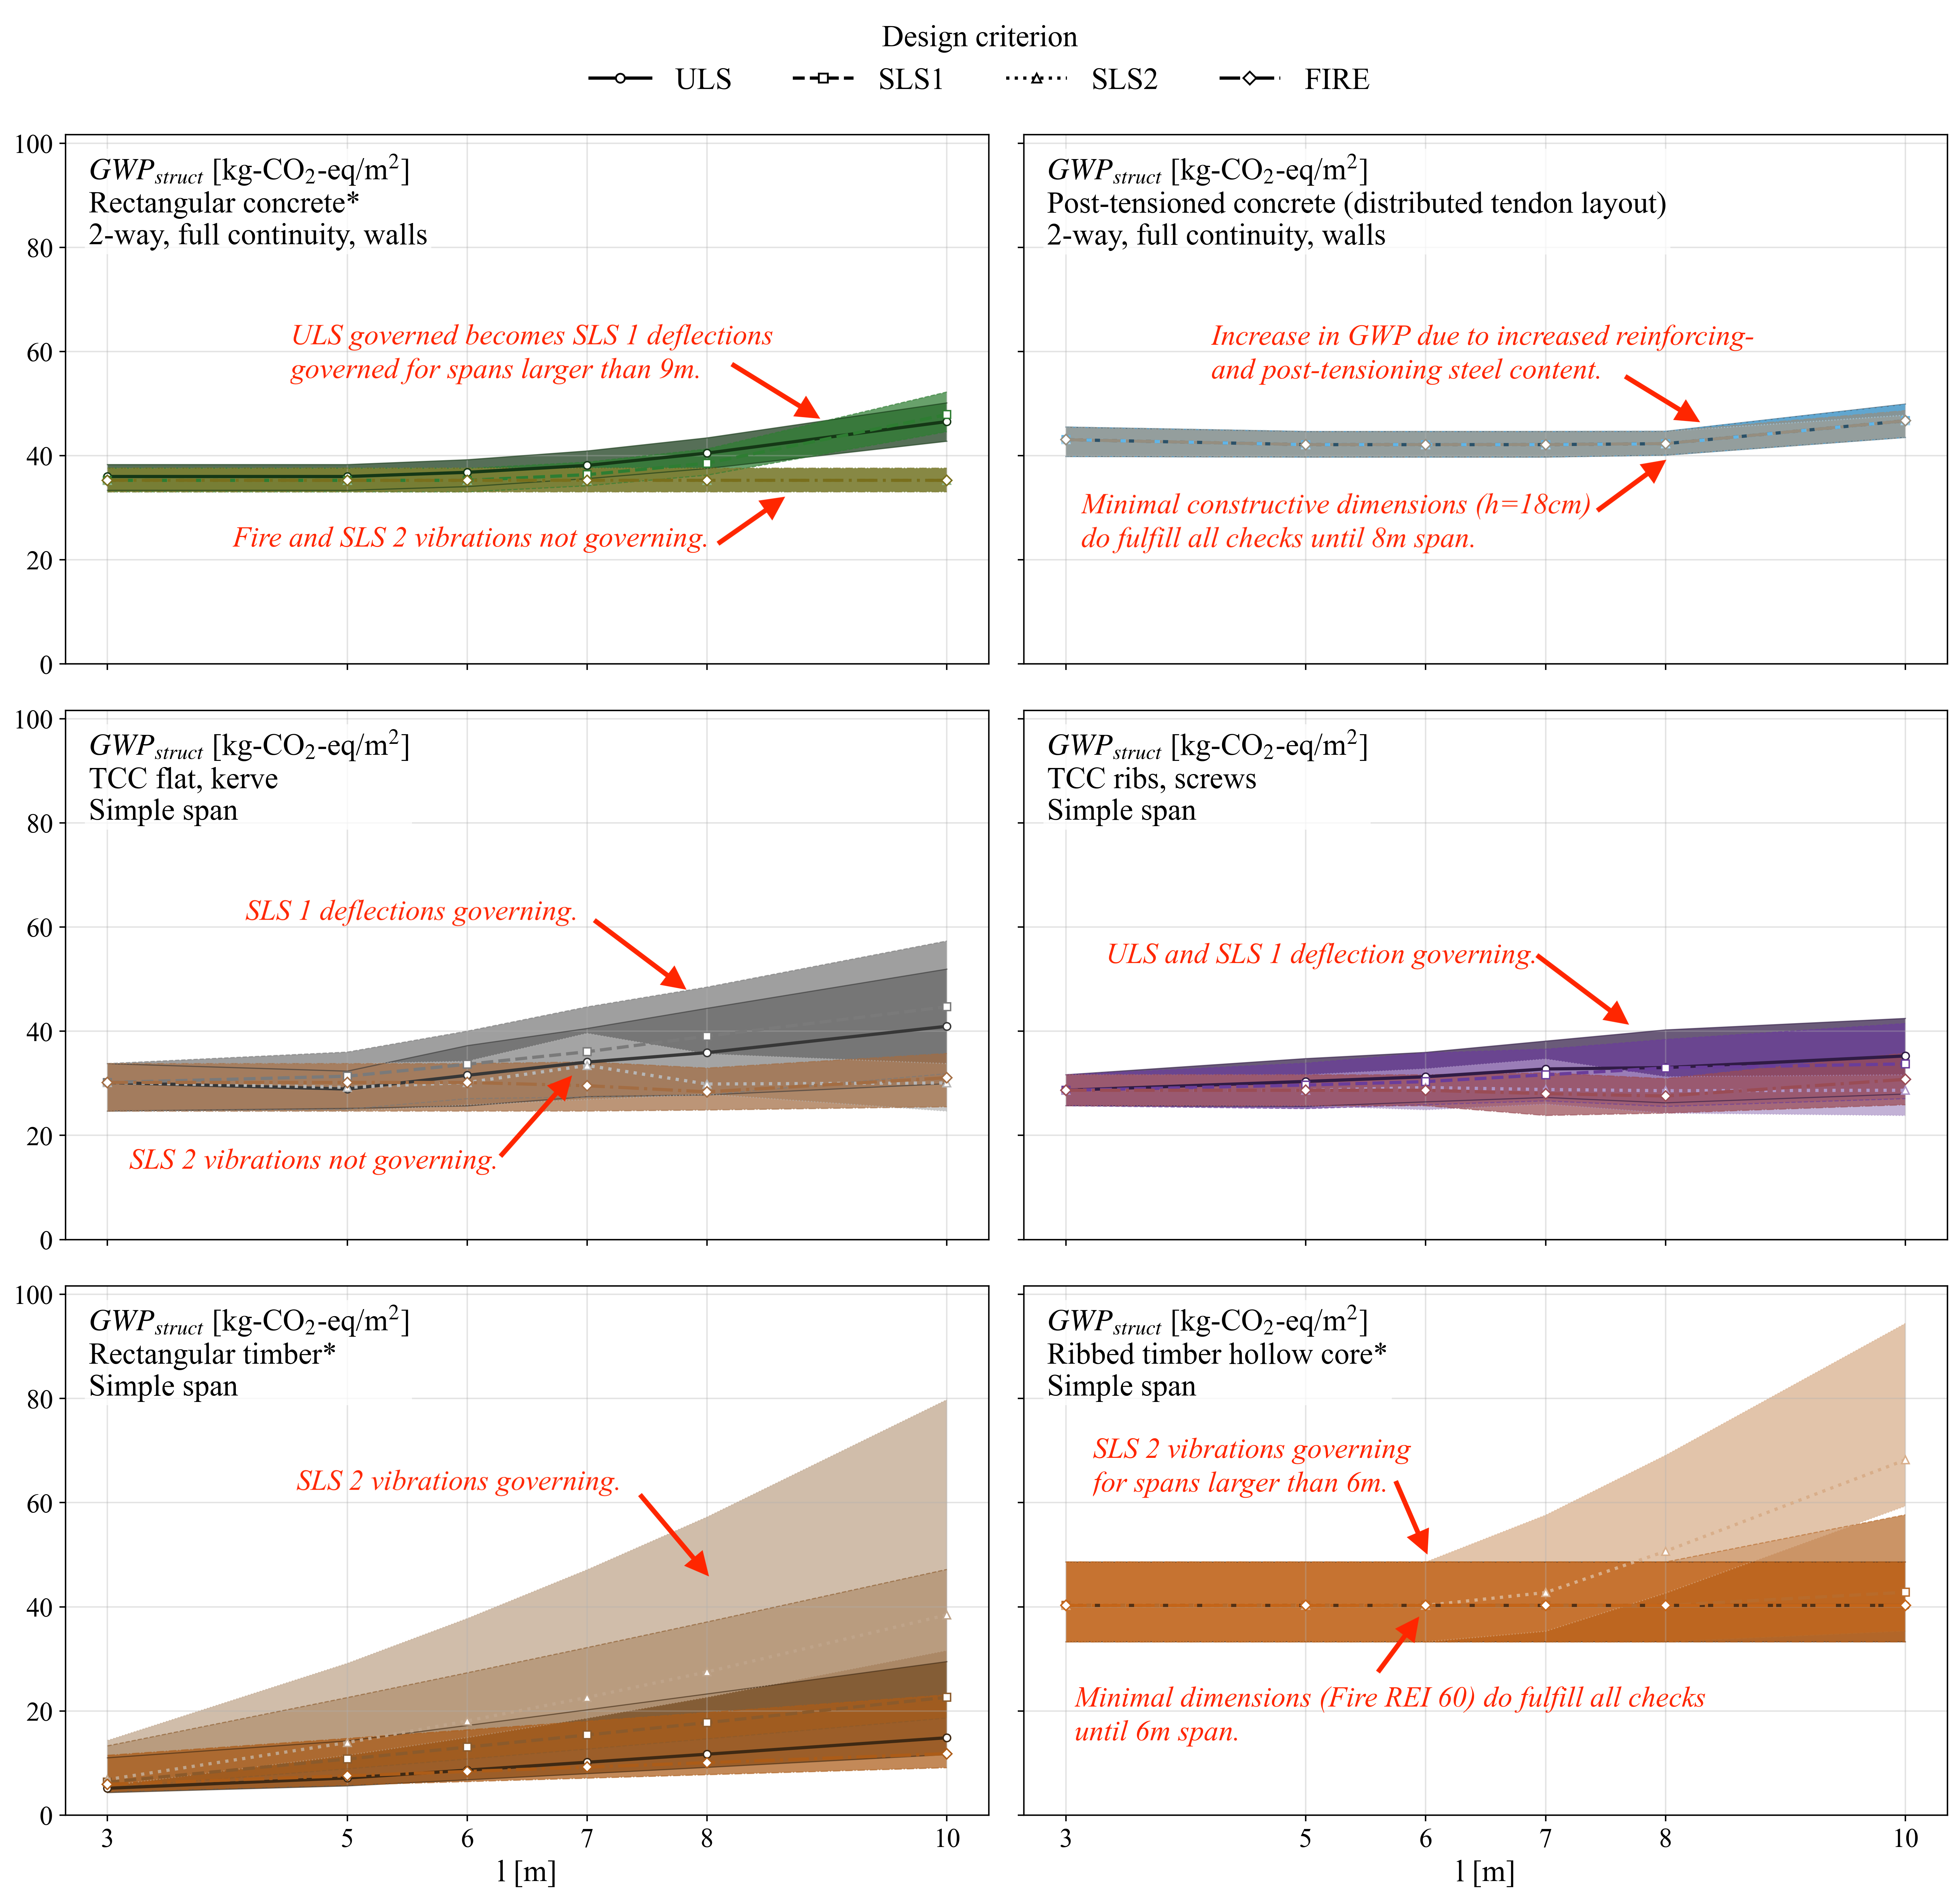
\includegraphics[width=1\textwidth]{IMAGES/final_single_residential_GWP_struct.png}
    \caption{GWP required to fulfil each respective design criterion of the structural cross-section for the residential case.}
    \label{fig:final_single_residential_GWP_struct}
\end{figure}

Figure~\ref{fig:final_single_residential_GWP_struct} shows the $GWP_{\mathrm{struct}}$ required by each system to fulfil the respective design criterion for the residential case. The values refer to the structural cross-section only, while the additional load of the floor build-up is already included in the structural model.

For the rectangular reinforced concrete slab, the governing criteria are ULS and SLS~1 deflection. Vibration and fire requirements are already fulfilled by the minimum dimensions and therefore do not lead to an increase over the investigated span range. SLS~1 deflection becomes governing only for spans larger than approximately $9,\mathrm{m}$. In engineering practice, deflection is often expected to govern the design \cite{Kaufmann2024_WhitePaper}. However, the present model set-up uses a favourable static system, with a rectangular layout, wall supports, two-way load transfer, and full continuity, which improves the deflection behaviour.

For the post-tensioned concrete slab, the results are governed by minimum detailing dimensions up to a span of approximately $8,\mathrm{m}$. For larger spans, $GWP_{\mathrm{struct}}$ increases due to the higher reinforcement and post-tensioning steel content required to satisfy the ULS design state. Compared with the conventionally reinforced concrete slab, SLS~1 deflection does not become governing. This confirms the intended serviceability improvement achieved through post-tensioning \cite{Rombach2010}.

\newpage
For the rectangular timber slab, SLS~2 vibration requirements govern over the investigated span range. Consequently, the available reserves in ULS, fire, and SLS~1 deflection cannot be exploited. For the ribbed timber hollow-core system, the minimum dimensions required to fulfil the REI~60 fire requirement govern up to a span of approximately $6,\mathrm{m}$. Beyond this span, SLS~2 vibration requirements also become governing. It can therefore be concluded that the dimensions of timber sections need to be increased primarily to satisfy vibration criteria.

For the timber--concrete composite systems, the SLS~2 vibration criterion does not become governing. This supports the improved vibration behaviour of TCC systems reported in the literature \cite{proHolz2012_Zuschnitt45}. Instead, the governing criteria are ULS and SLS~1 deflection.

Overall, cross-sections containing concrete show a smaller variation in $GWP_{\mathrm{struct}}$ across the design states. This supports that concrete contributes to the functional performance of floor systems, since its stiffness, mass and fire resistance can help satisfy several design requirements simultaneously. These functional advantages also help explain the continued prevalence of concrete floor systems in practice \cite{Priore2024_CarbonImpactSlabs, Ammann2024}.

\newpage
\subsection{Best cross-section}
Figure~\ref{fig:final_cross_sections_residential_6m} shows the best \(GWP_{tot}\) cross-sections for the residential case at a span of \(6\,\mathrm{m}\). The breakdown of GWP, cost and construction time underlines the importance of assessing the complete floor system rather than the structural cross-section alone. Across all residential systems, the acoustic floor build-up contributes a substantial share of \(GWP_{tot}\), construction cost, and construction time. 

\begin{figure}[H]
    \centering
    
\includegraphics[width=1\textwidth]{IMAGES/final_cross_sections_residential_6m.png}
    \caption{Best \(GWP_{tot}\) cross-sections for the residential case at a span of \(6\,\mathrm{m}\).}
    \label{fig:final_cross_sections_residential_6m}
\end{figure}


\subsection{Comparison of residential floor systems}
Figure~\ref{fig:final_env_comparison_residential} compares the residential floor systems over the investigated span range and illustrates the variation resulting from the considered material and product datasets. 
\begin{figure}[H]
    \centering
    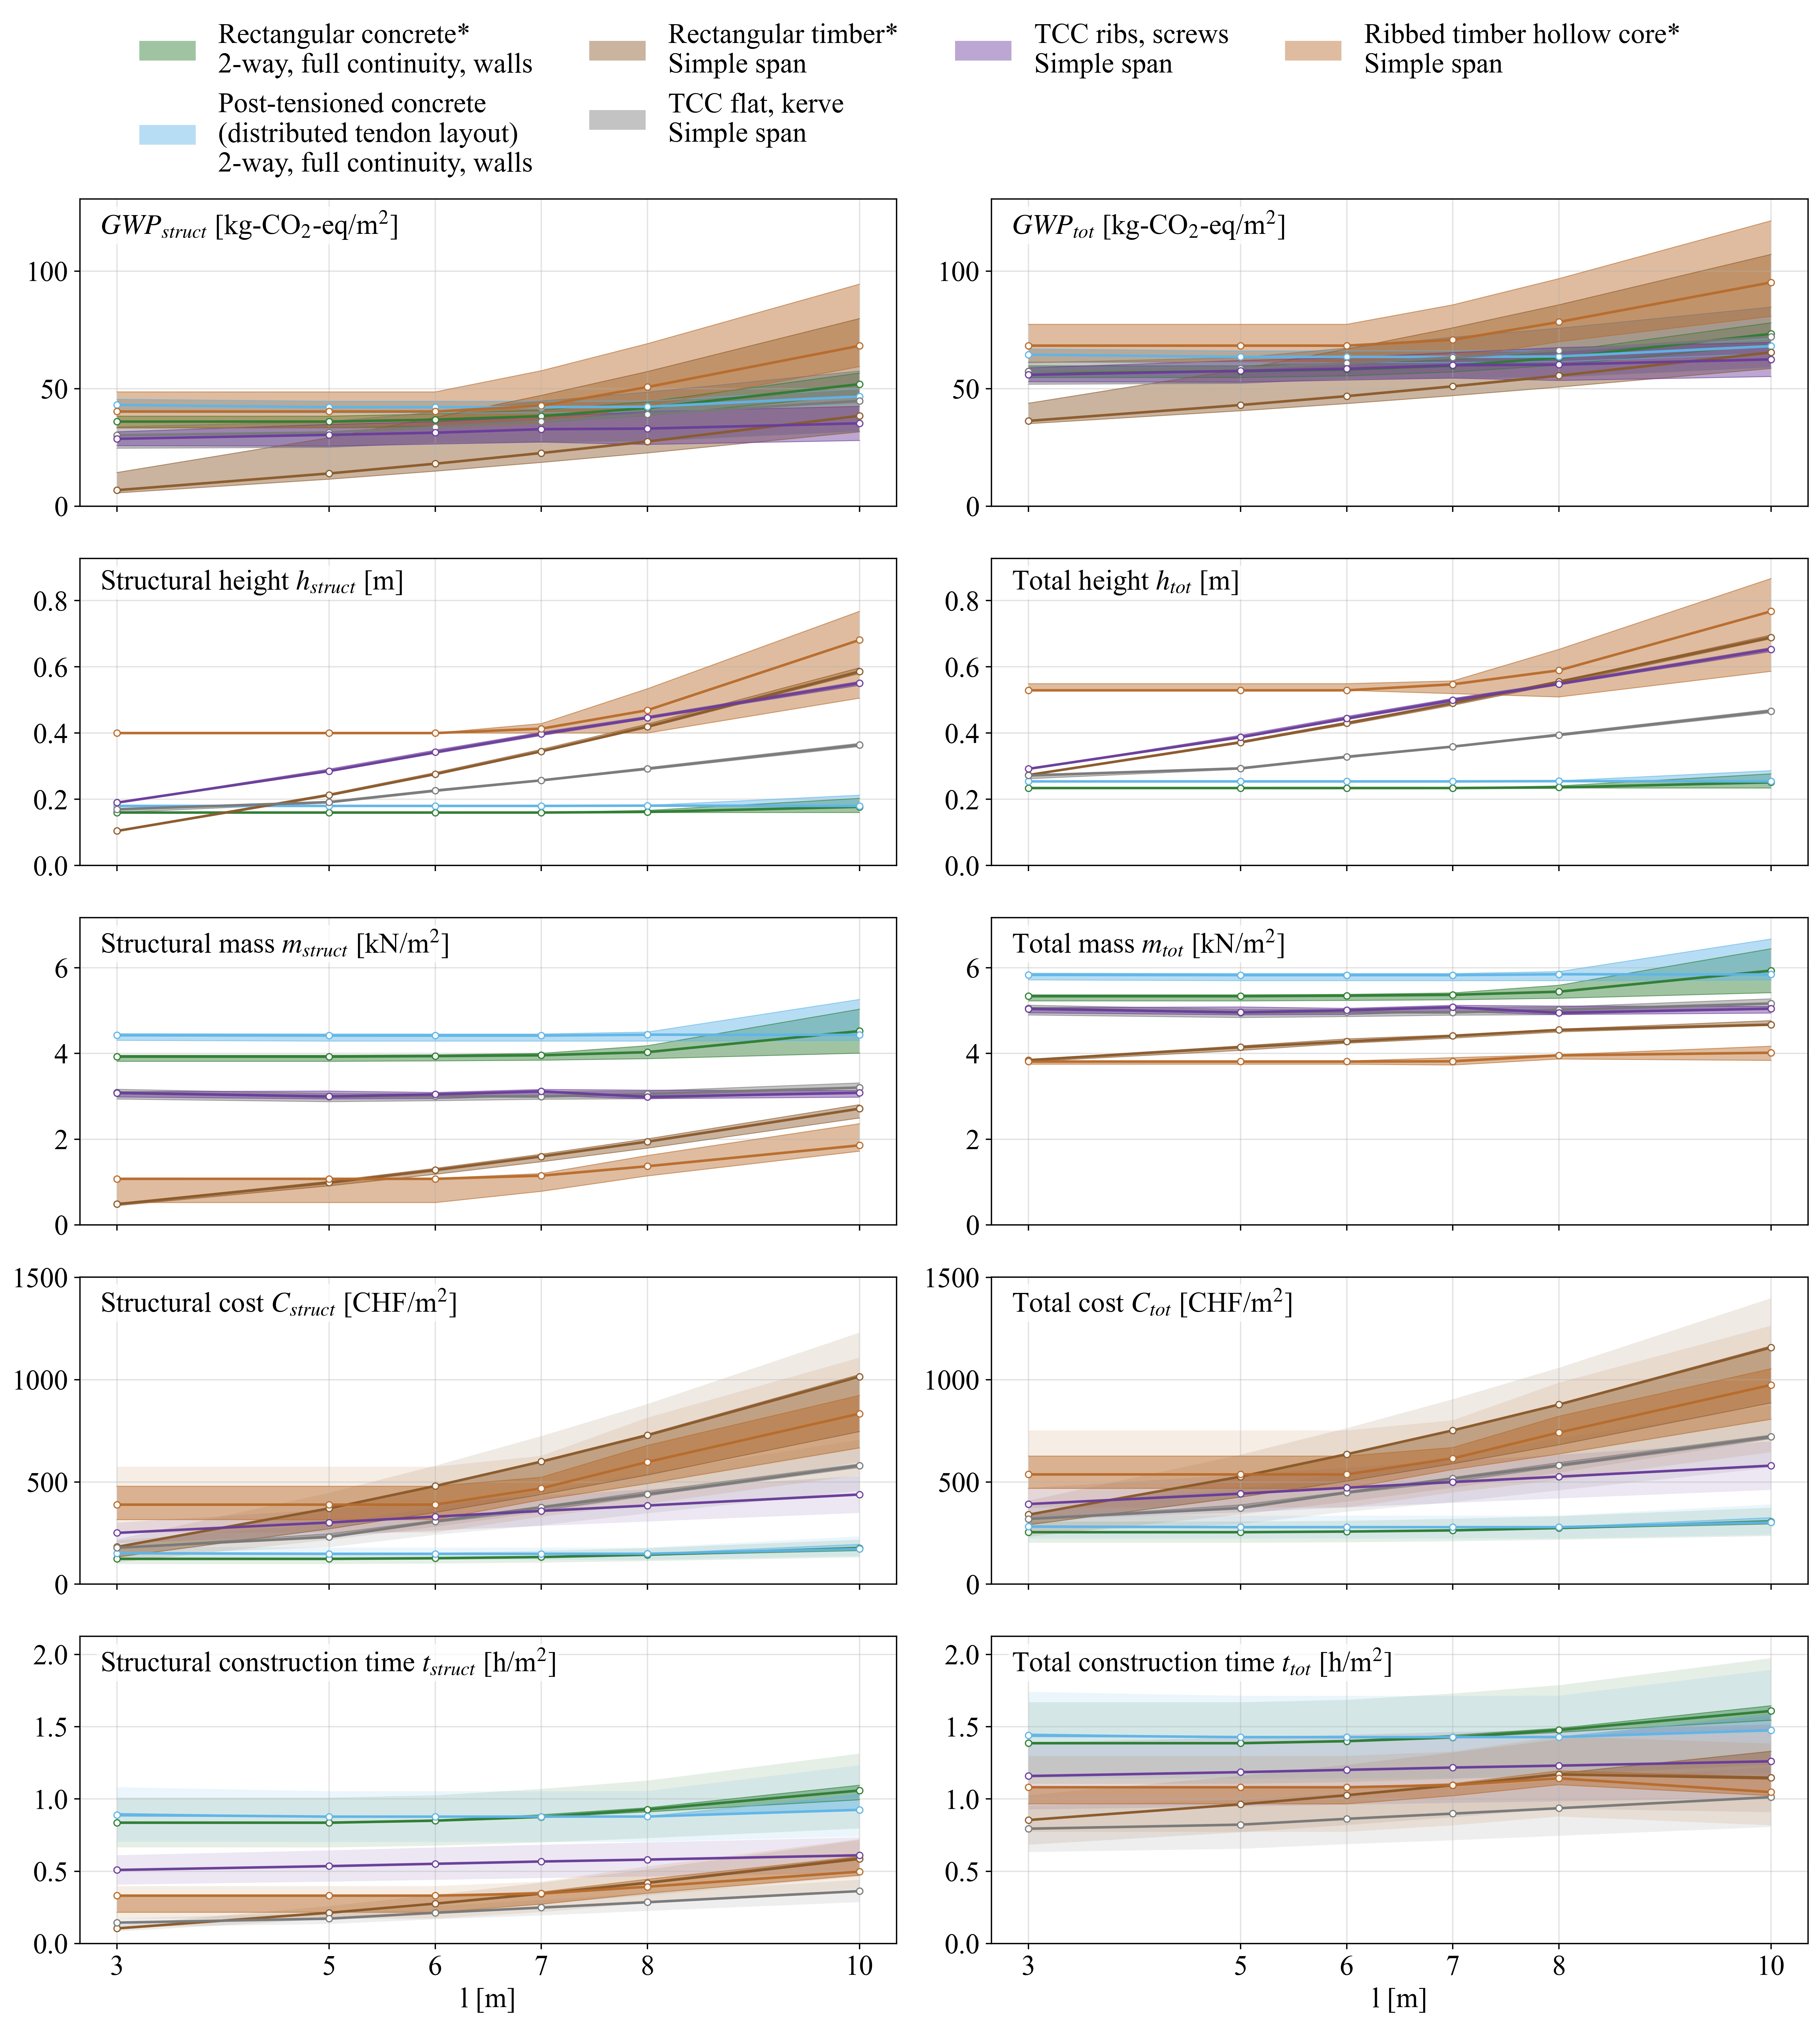
\includegraphics[width=1\textwidth]{IMAGES/final_env_comparison_residential.png}
    \caption{Comparison according to sustainability assessment criteria of selected floor systems for residential buildings.}
    \label{fig:final_env_comparison_residential}
\end{figure} 

Figure~\ref{fig:uq_pairwise_scores_Residential} complements this comparison by a pairwise comparison that accounts for overlaps between the resulting performance ranges. A pairwise score of \(0.8\) indicates that the respective system has an average probability of \(80\,\%\) of outperforming the systems positioned below it in the figure.
\begin{figure}[H]
    \centering
    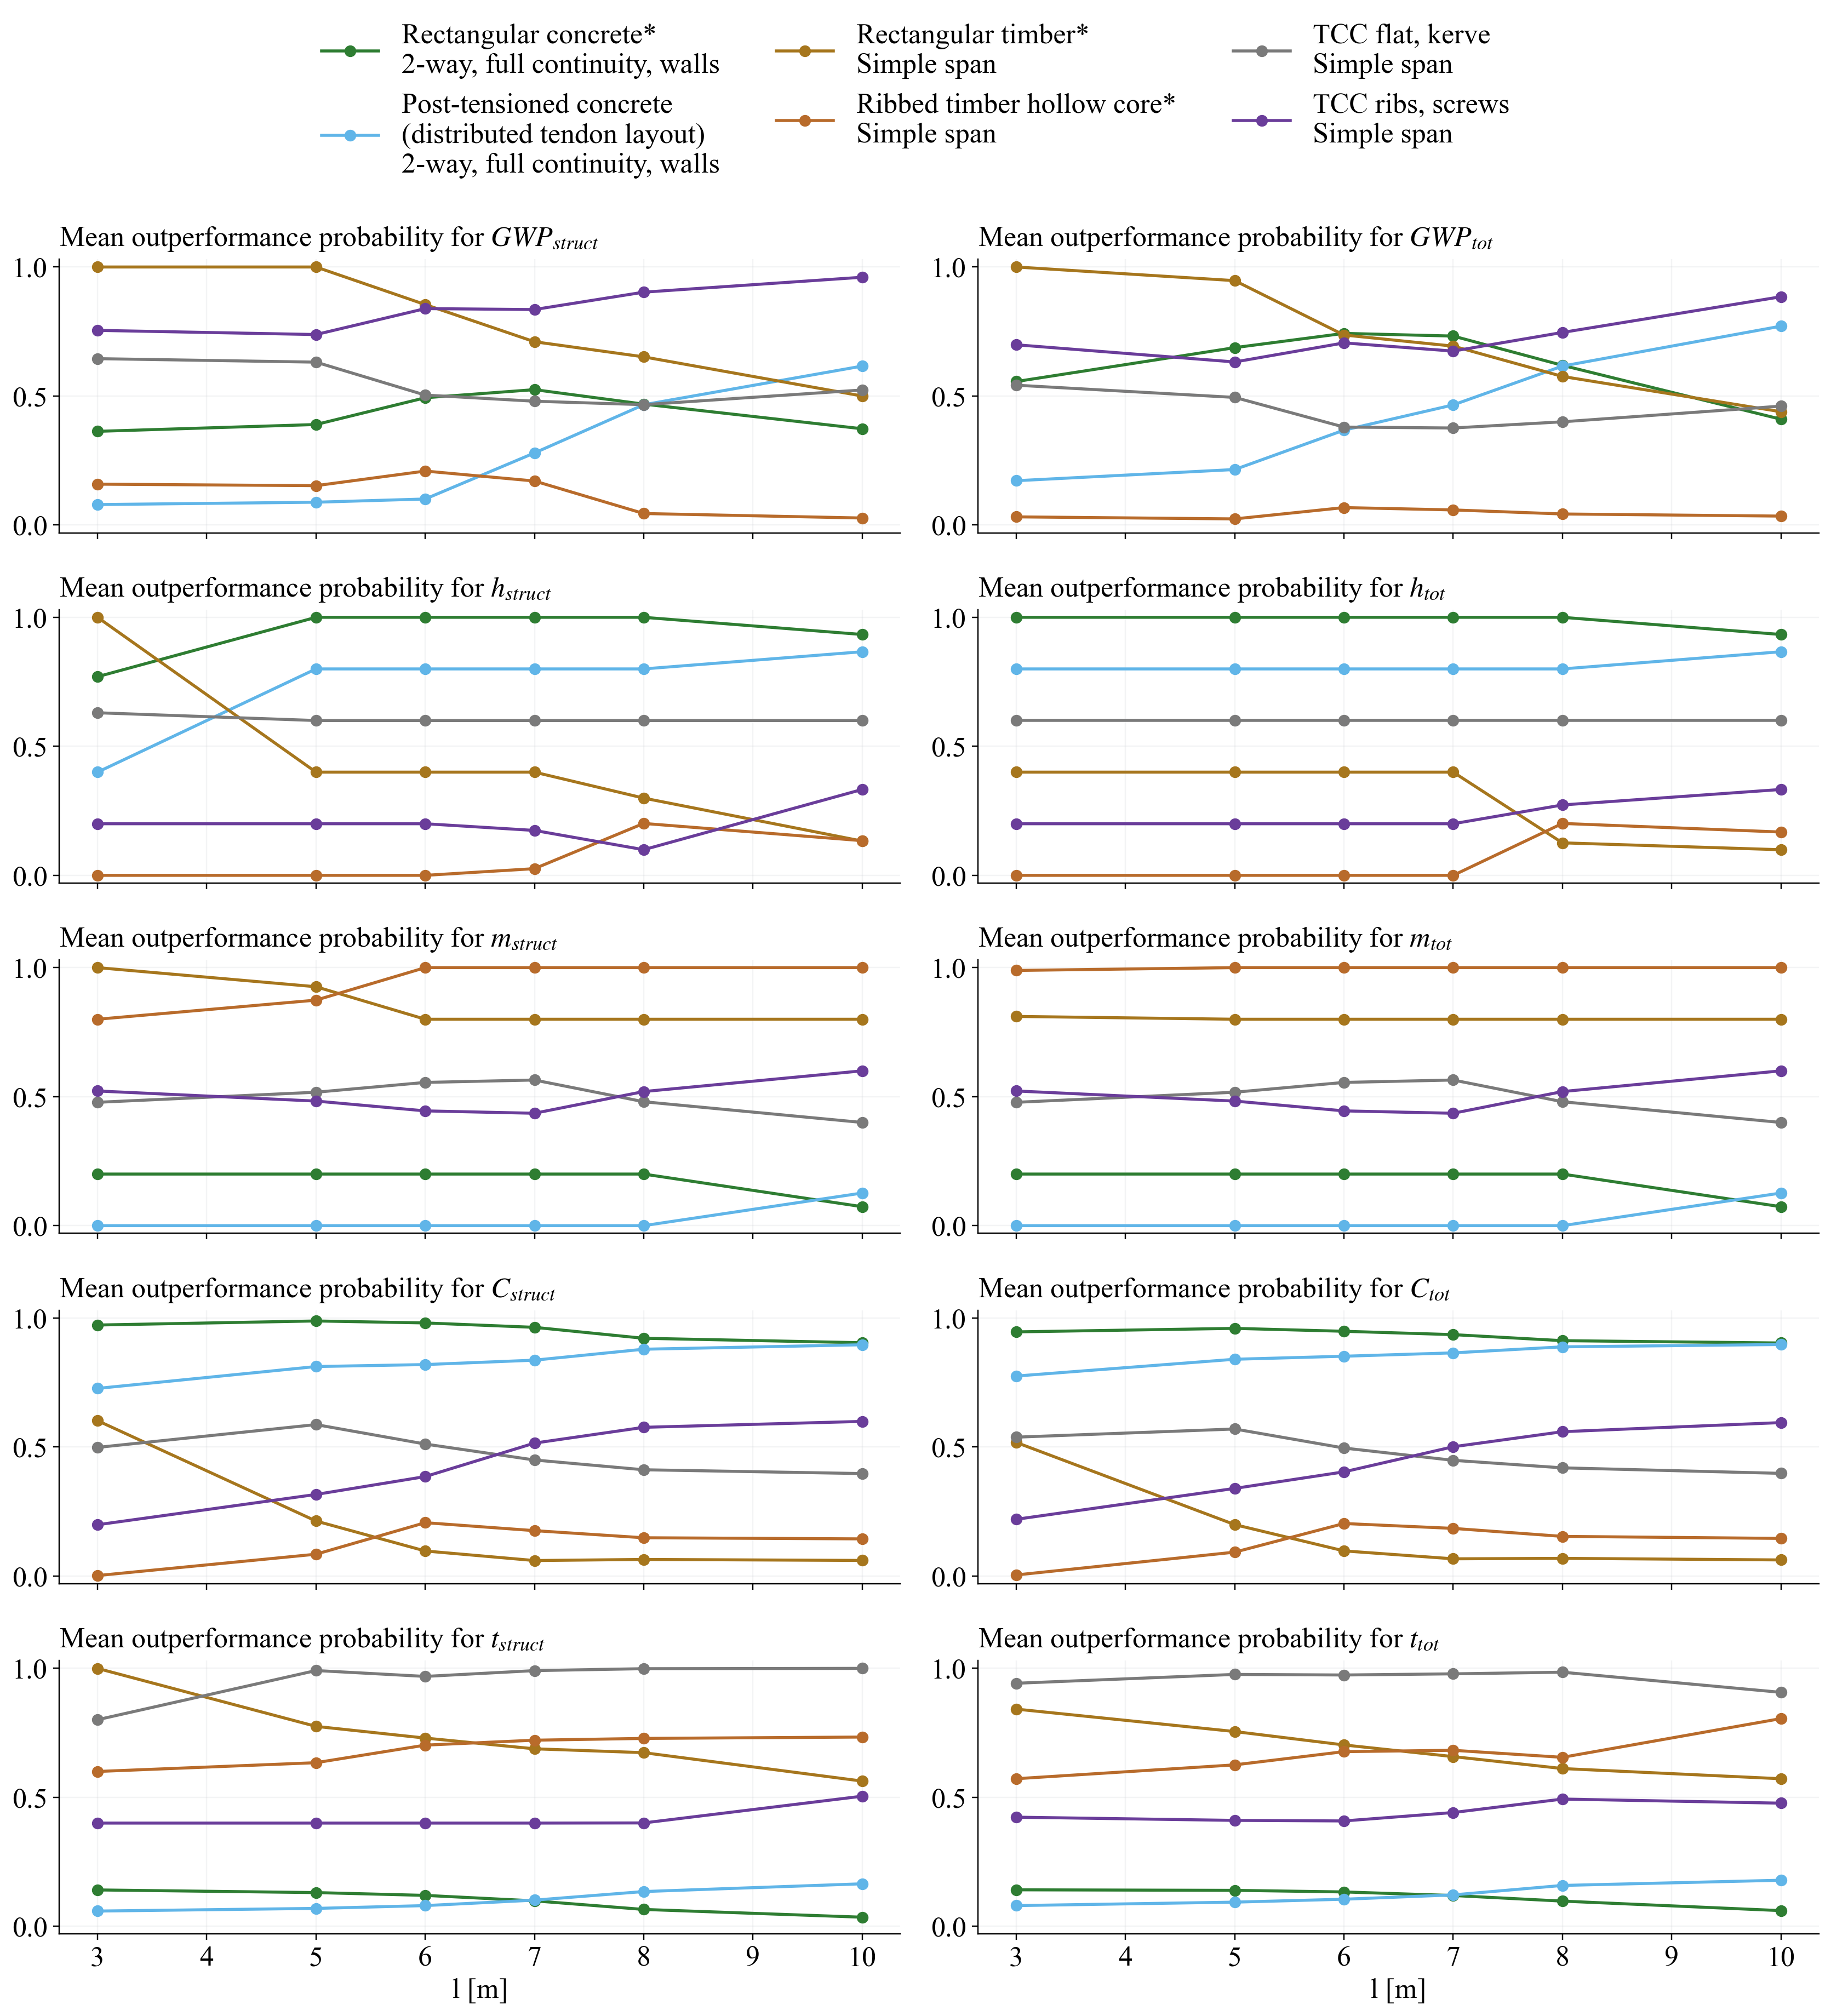
\includegraphics[width=1\textwidth]{IMAGES/uq_pairwise_scores_Residential.png}
    \caption{Pairwise comparison according to sustainability assessment criteria of selected floor systems for residential buildings.}
    \label{fig:uq_pairwise_scores_Residential}
\end{figure}

\newpage
Both figures distinguish between the structural cross-section and the total floor system, with the latter additionally accounting for the acoustic floor build-up. This distinction is particularly important for timber and timber--concrete composite systems, whose acoustic build-ups are generally heavier, deeper, and more emission-intensive than those of concrete systems. This observation is consistent with the multilayer timber floor configurations documented by Lignum \cite{LignumData_Decken}.


\subsubsection{Global warming potential}

Rectangular timber achieves the lowest structural GWP for spans between \(3\) and \(5\,\mathrm{m}\). For larger spans, its vibration behaviour increases the required dimensions notably, resulting in the strongest increase in GWP over the span.
At intermediate spans of approximately \(6\) to \(7\,\mathrm{m}\), rectangular reinforced concrete becomes the best-performing system. Here, reinforced concrete uses its highly efficient two-way structural system with full continuity. Above approximately \(7\,\mathrm{m}\), ribbed TCC and post-tensioned concrete become increasingly competitive. This is consistent with the span range in which post-tensioning is generally considered structurally effective \cite{Rombach2010}.

Ribbed TCC achieves particularly low structural GWP at longer spans because its structurally efficient ribbed cross-section reduces material consumption. This advantage comes at the cost of a substantially increased construction depth. Flat TCC exhibits slightly higher structural GWP, with the difference between the two TCC systems increasing with span.

The pairwise comparison modifies the interpretation of these span limits. When all total-system criteria are considered together, rectangular timber is only the clear overall winner at \(3\,\mathrm{m}\). Flat TCC obtains the highest total pairwise score at \(5\,\mathrm{m}\) and again at \(8\,\mathrm{m}\), mainly because it combines competitive GWP with moderate height and short construction time. Rectangular reinforced concrete narrowly leads the total pairwise comparison at \(6\) and \(7\,\mathrm{m}\), where its low cost and low construction height compensate for its higher GWP. At \(10\,\mathrm{m}\), ribbed TCC becomes the highest-ranked system, although post-tensioned concrete and flat TCC remain close alternatives. The span recommendations should therefore be understood as robust multi-criteria ranges rather than as direct transitions between the lowest deterministic \(GWP_{tot}\) values.

The ribbed timber hollow-core system exhibits the highest structural GWP across most of the investigated span range. At shorter spans, this can be explained by the governing minimum dimensions required by the simplified fire-design model. A more refined fire verification could reveal further potential. In addition, the result is strongly influenced by the assumed hollow-core insulation. It must therefore be interpreted cautiously, as alternative insulation products could substantially affect the environmental performance.

\subsubsection{Height}
The slender rectangular concrete achieves the lowest total floor height until a span of \(8\,\mathrm{m}\). The post-tensioned concrete is limited by its geometrical minimum dimensions due to detailing of the anchorage and post-tensioning tendons. However, it surpasses the rectangular concrete cross-section for spans larger than \(8\,\mathrm{m}\).

Rectangular timber remains competitive up to approximately \(5\,\mathrm{m}\) and acceptable between \(5\) and \(7\,\mathrm{m}\), but its required depth increases substantially at longer spans. Flat TCC achieves a lower total height than the pure timber systems and ribbed TCC. Ribbed TCC provides high material efficiency but requires a considerably greater structural depth, particularly at longer spans.

The results also demonstrate the relevance of floor height as a sustainability assessment criterion. According to the Building and Zoning Regulations of the City of Zurich, the permissible building height in zone W5 is generally limited to \(18\,\mathrm{m}\) \cite{StadtZuerich_Bauordnung_700100}. Assuming a clear room height of \(2.4\,\mathrm{m}\), six storeys are possible only if the total floor depth remains below \(0.6\,\mathrm{m}\). Floor height can therefore directly affect the achievable service area. This is critical when trying to achieve a high service area in relation to the total invested carbon of the building \cite{Kaufmann2024_WhitePaper}. For the investigated example, imposing \(h_{\mathrm{tot}}\leq 0.6\,\mathrm{m}\) would exclude rectangular timber, ribbed timber hollow-core, and ribbed TCC solutions at spans above approximately \(7\,\mathrm{m}\), showing the importance of this sustainability assessment criterion.

\subsubsection{Mass}
At the structural level, the timber-based systems are substantially lighter than the concrete systems. However, this difference decreases when the complete floor system is considered because the timber and TCC systems require relatively heavy acoustic floor build-ups. Consequently, the total mass of the investigated systems generally lies between approximately \(400\) and \(600\,\mathrm{kg/m^2}\), which is consistent with floor configurations documented by Lignum \cite{Lignum2021_HBT1}.

Thus, for buildings founded on soil with sufficient bearing capacity, differences in floor mass are unlikely to cause major changes in the environmental impact of the substructure. The relevance of mass may increase under poor ground conditions.

Additionally, mass also affects seismic actions. However, this benefit cannot be evaluated independently of the height. Here, the lightweight systems require greater floor depths, potentially increasing the total building height and altering the seismic response. A conclusive building-level assessment therefore requires the combined consideration of floor mass and structural height. 

Most importantly, the magnitude of the indirect influences on the foundation and the lateral load-resisting structural system depends on the number of storeys. For a conventional residential building with fewer than six storeys, mass is therefore proposed to be handled as a secondary sustainability assessment criterion.

\subsubsection{Construction cost}
Rectangular concrete achieves the lowest construction cost until spans of \(9\,\mathrm{m}\). This reflects both the economic efficiency of established concrete construction processes and the low material price of concrete. It must be noted that post-tensioned concrete is economically competitive across all spans and even surpasses traditional reinforced concrete above spans of \(9\,\mathrm{m}\). This is attributed to the reduced total steel content of the post-tensioned concrete.

The timber systems are among the most expensive alternatives. This result should be interpreted cautiously because their unit price is defined per cubic metre and implicitly accounts for connections and fabrication. In practice, the relative contribution of these components may decrease as member dimensions increase. The present model may therefore overestimate the cost of large timber cross-sections.

Ribbed TCC is more expensive than flat TCC up to approximately \(7\,\mathrm{m}\). This is primarily caused by the screw connectors, each of which is explicitly included in the cost model. At longer spans, the material efficiency of the ribbed system becomes more influential.

Post-tensioned concrete becomes economically competitive with conventional reinforced concrete at approximately \(8\,\mathrm{m}\) and above. At these spans, its lower material demand increasingly compensates for the additional post-tensioning components.

\subsubsection{Construction time}
Flat TCC exhibits a comparatively short construction time. The timber component serves as permanent formwork, while the notched connectors can be prefabricated before installation \cite{Morkoetter2021_HBVDecken}.

Ribbed TCC requires more construction time than flat TCC at shorter and intermediate spans because of the larger number of individually installed screw connectors \cite{Morkoetter2021_HBVDecken, Wuerth2021_HolzBetonVerbund}.

Rectangular timber also performs favourably regarding construction time, even outperforming the flat TCC cross-section at a span of \(3\,\mathrm{m}\). The steep increase in construction time for the timber cross-section is, however, an indication that assuming cost and construction time to depend only on the volume used for timber cross-sections is not adequate. For more precise modelling, it is proposed to assume a fixed installation cost and construction time, accompanied by a value per volume to account for higher material usage.

Post-tensioned concrete outperforms conventional reinforced concrete at spans above \(7\,\mathrm{m}\). The additional effort required for tendon installation is increasingly offset by the reduced cross-sectional dimensions and material quantities. The model does not account for the reduced propping time enabled by post-tensioning. Due to the compensation of permanent loads, the formwork can be removed earlier, additionally improving construction progress and making the overall project economically more competitive.



\section{Office case}
\subsection{Analysis of slab systems} 
Figure~\ref{fig:final_single_office_GWP_struct} shows all systems of the office case and compares the required \(GWP_{struct}\) needed to fulfil the respective design criteria. Since only concrete systems are considered, neither the SLS~2 vibration criterion nor the fire criterion becomes governing. 

\begin{figure}[H]
    \centering
    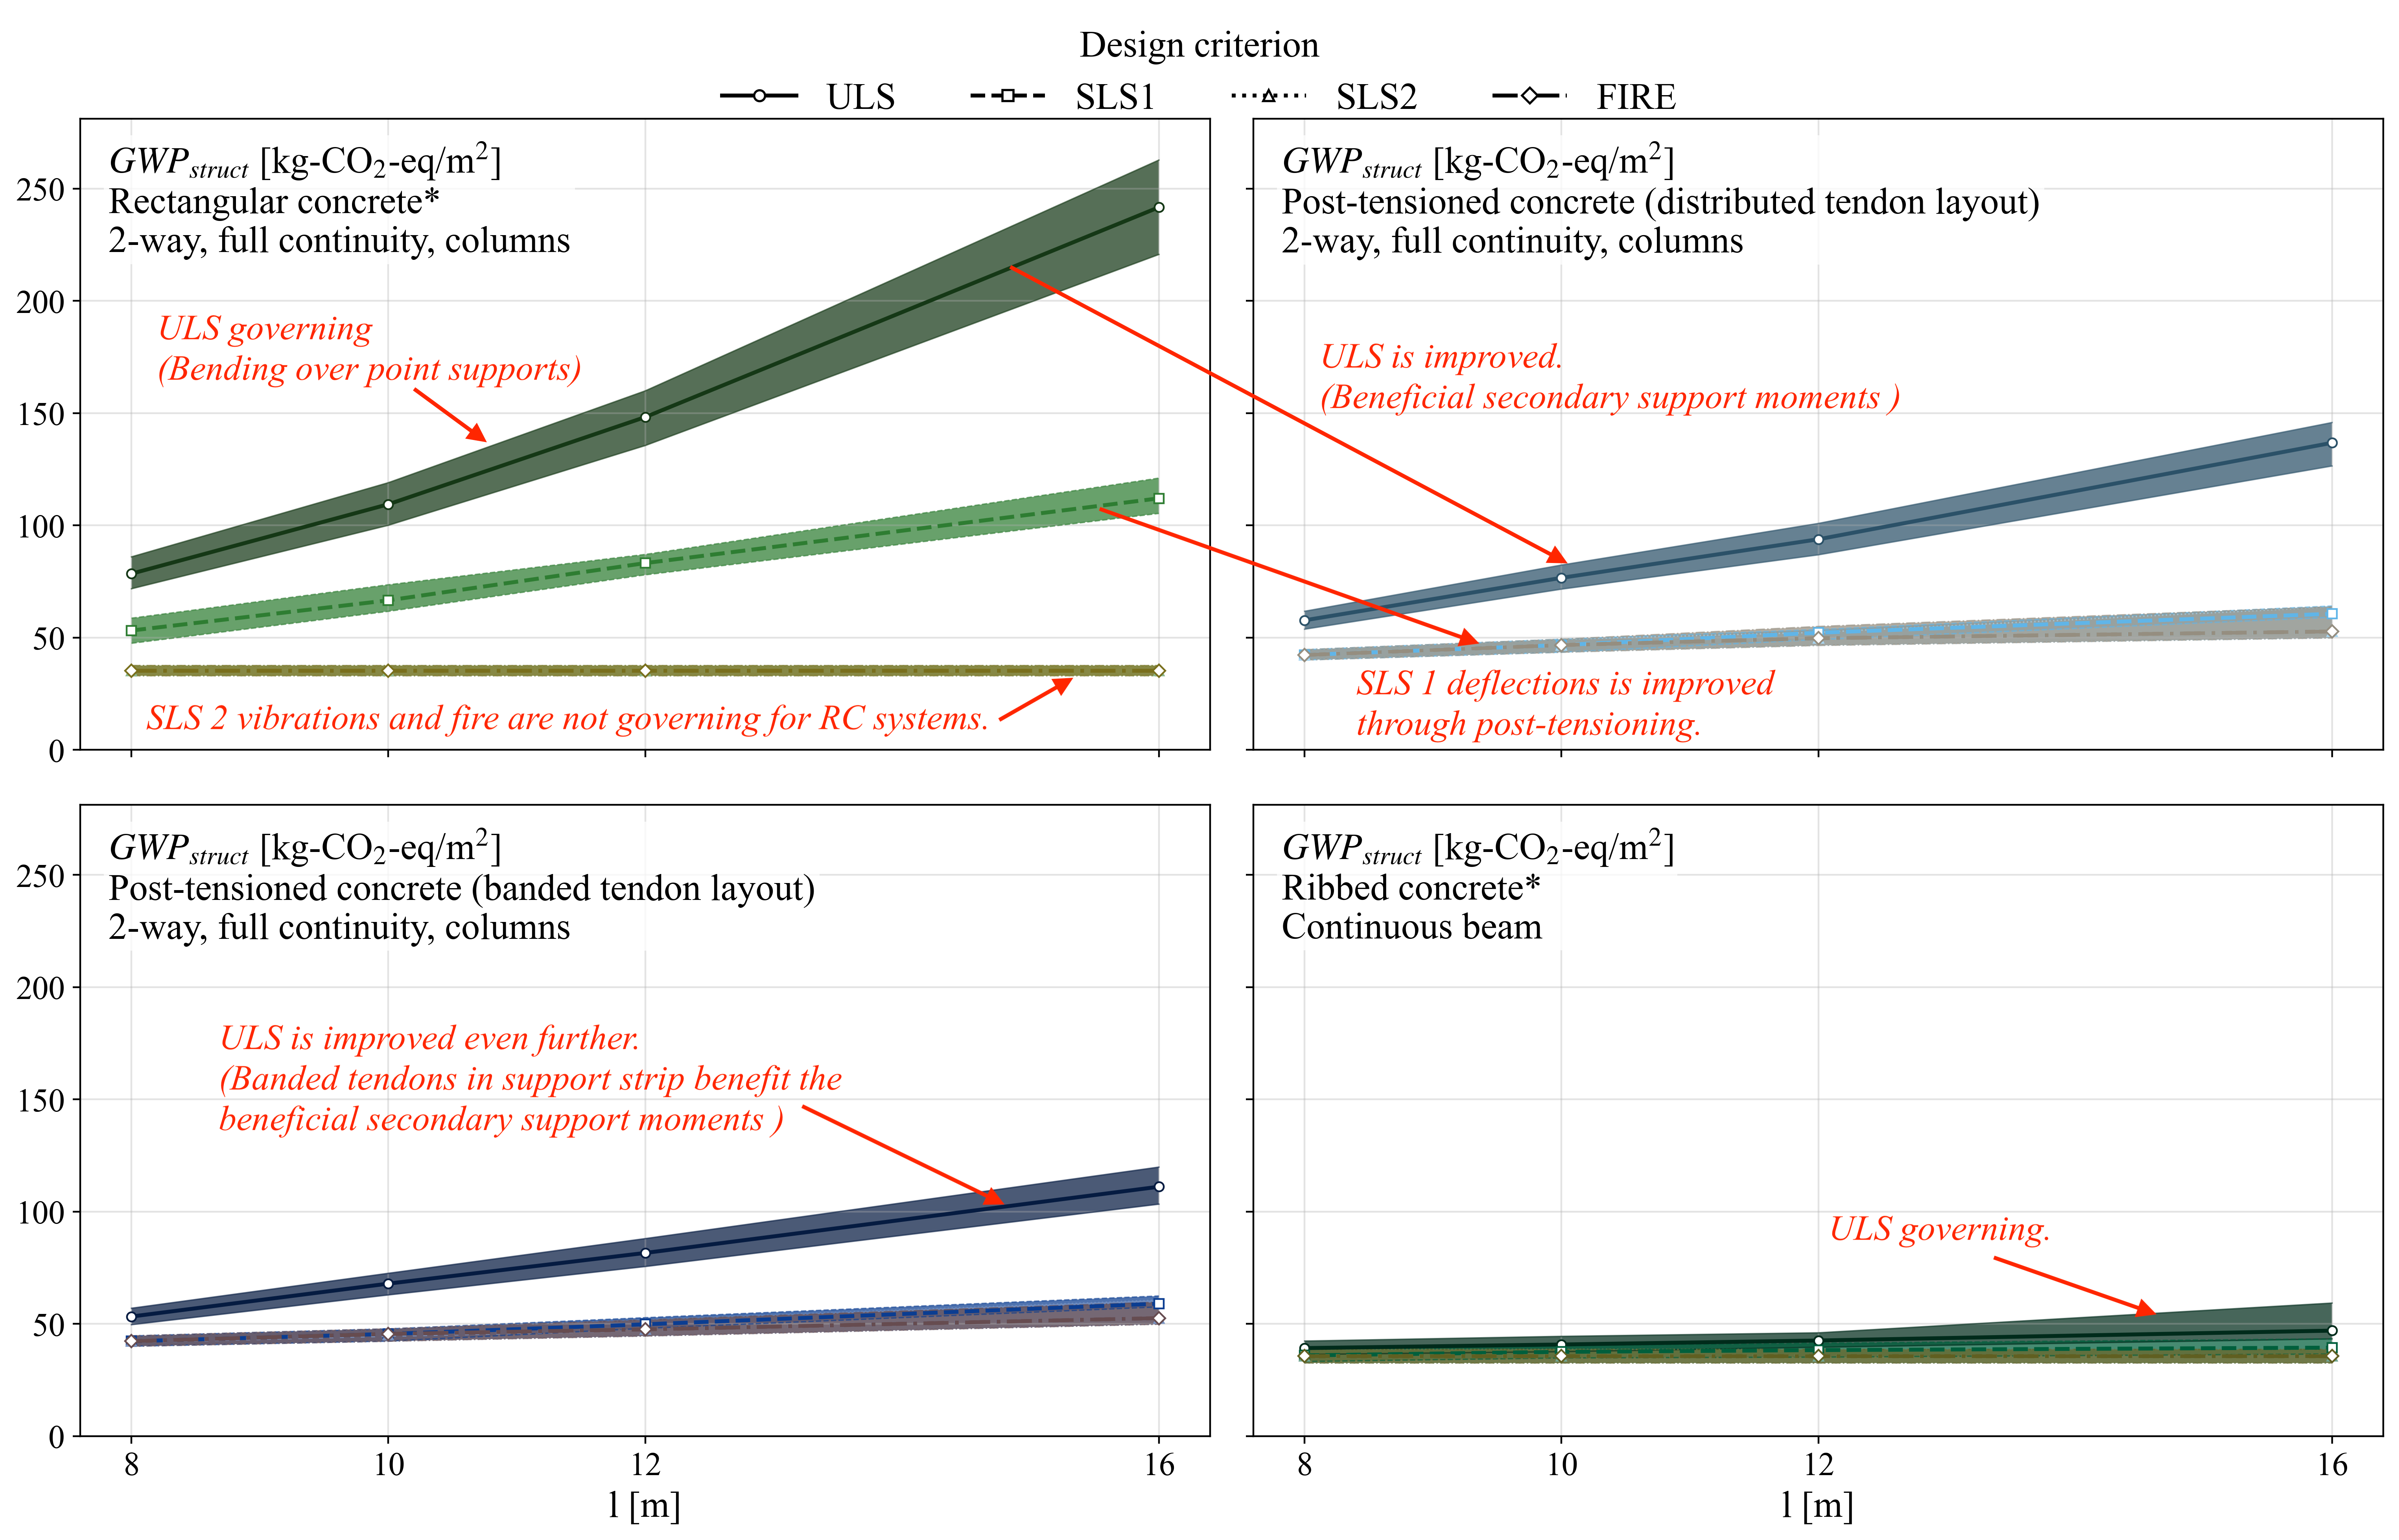
\includegraphics[width=1\textwidth]{IMAGES/final_single_office_GWP_struct.png}
    \caption{GWP required to fulfil each respective design criterion of the structural cross-section for the office case.}
    \label{fig:final_single_office_GWP_struct}
\end{figure}


\newpage
For the point-supported systems, namely the rectangular reinforced concrete and solid post-tensioned concrete slabs, ULS is governed by the negative bending moments over the supports. In the post-tensioned systems, the ULS demand is reduced by beneficial secondary moments generated above the columns. This effect is more pronounced for the banded tendon layout, as the tendons are concentrated within the column strips, where the governing ULS verifications are performed in the present model.
Additionally, the improved punching behaviour of post-tensioned slabs reduces the required amount of punching reinforcement, thereby lowering the GWP compared to conventionally reinforced slabs. Here, the banded layout also performs better, as the deviation forces of all tendons are assumed to counteract the punching load.

The comparison also shows that SLS~1 deflection requirements are improved when moving from conventional reinforced concrete to post-tensioned concrete. This is relevant because deflections may become critical at larger spans, particularly when serviceability limits are not only defined relative to the span, but also by absolute deformation limits. Such absolute limits can be important when non-structural elements, such as interior walls or finishes, cannot accommodate the resulting deflections for the longer compared office spans.

Ribbed concrete is also governed by ULS. However, the different design criteria lie comparatively close to each other, indicating that the system is structurally highly optimised. 

\newpage
\subsection{Best cross-section}
Figure~\ref{fig:final_cross_sections_office_12m} shows the best \(GWP_{tot}\) cross-sections for the office case at a span of \(12\,\mathrm{m}\). The reduced punching reinforcement demand of the post-tensioned systems is validated by their lower required punching shear reinforcement resistance \(V_{Rd,s}\) compared with the conventionally reinforced concrete slab.

\begin{figure}[H]
    \centering
    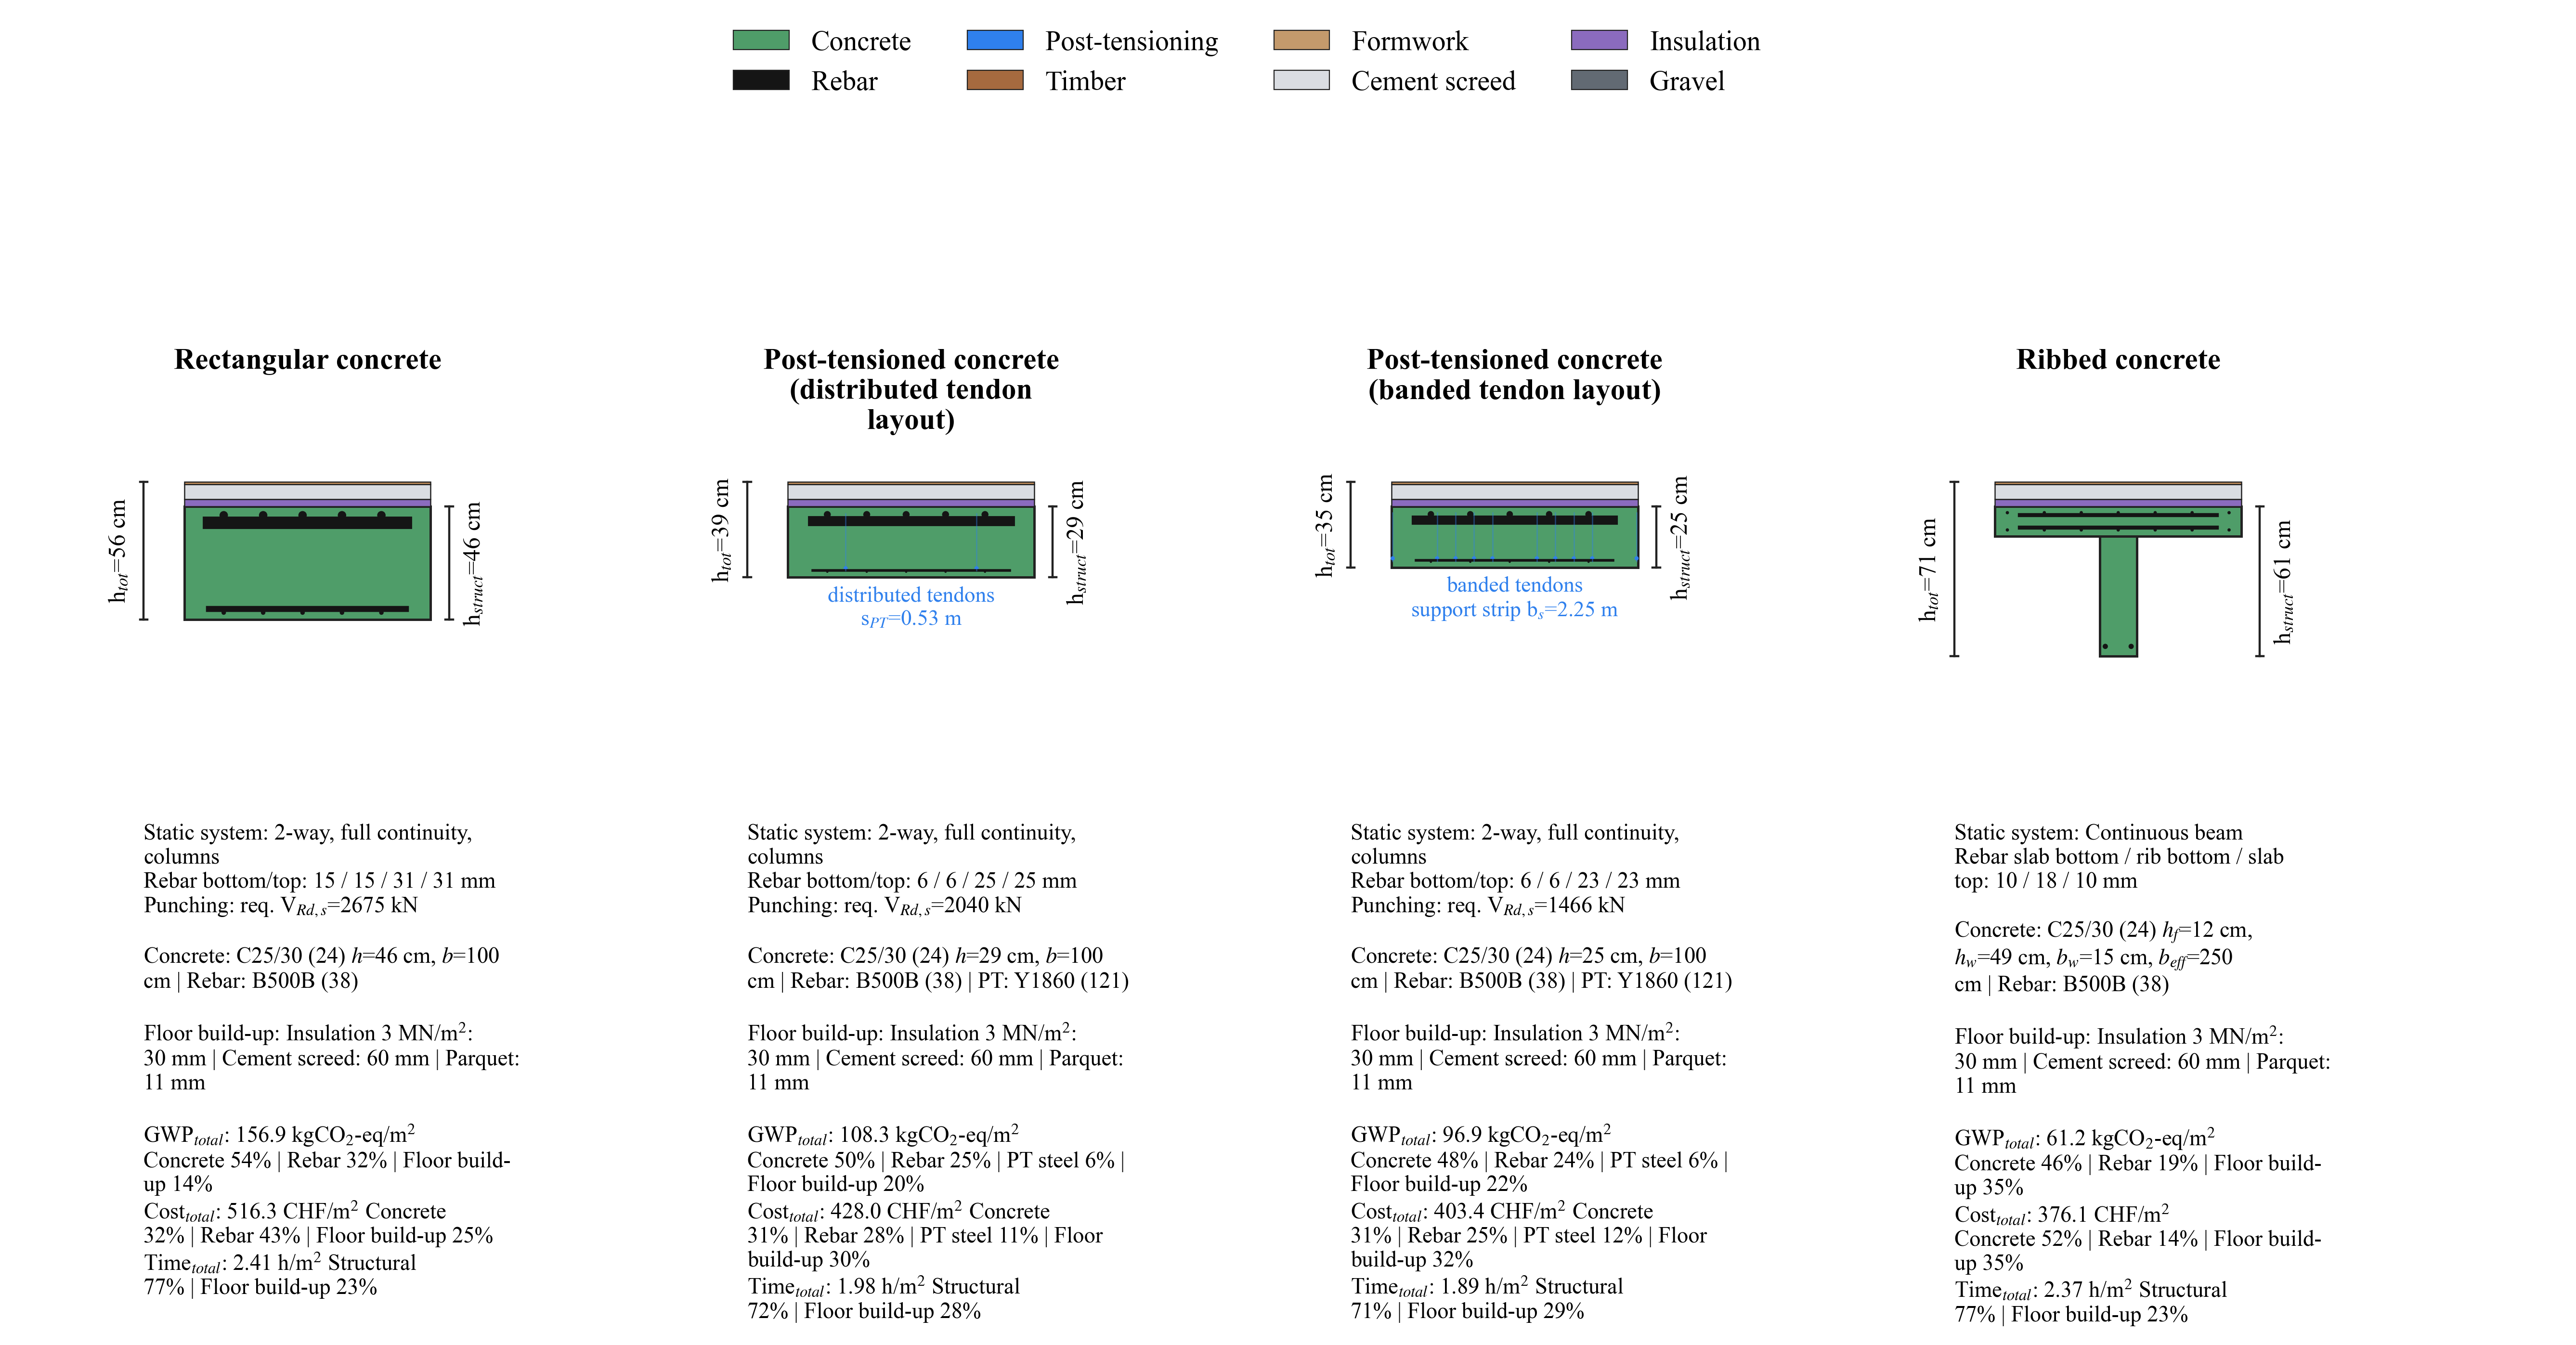
\includegraphics[width=1\textwidth]{IMAGES/final_cross_sections_office_12m.png}
    \caption{Best \(GWP_{tot}\) cross-sections for the office case at a span of \(12\,\mathrm{m}\).}
    \label{fig:final_cross_sections_office_12m}
\end{figure}

\newpage 
\subsection{Comparison of office floor systems}
The systems of the office case were compared in a similar manner to the residential case. Figure~\ref{fig:final_env_comparison_office} compares the office floor systems over the investigated span range and illustrates the variation resulting from the considered material and product datasets. Figure~\ref{fig:uq_pairwise_scores_Office} complements this comparison by the pairwise comparison. 
\begin{figure}[H]
    \centering
    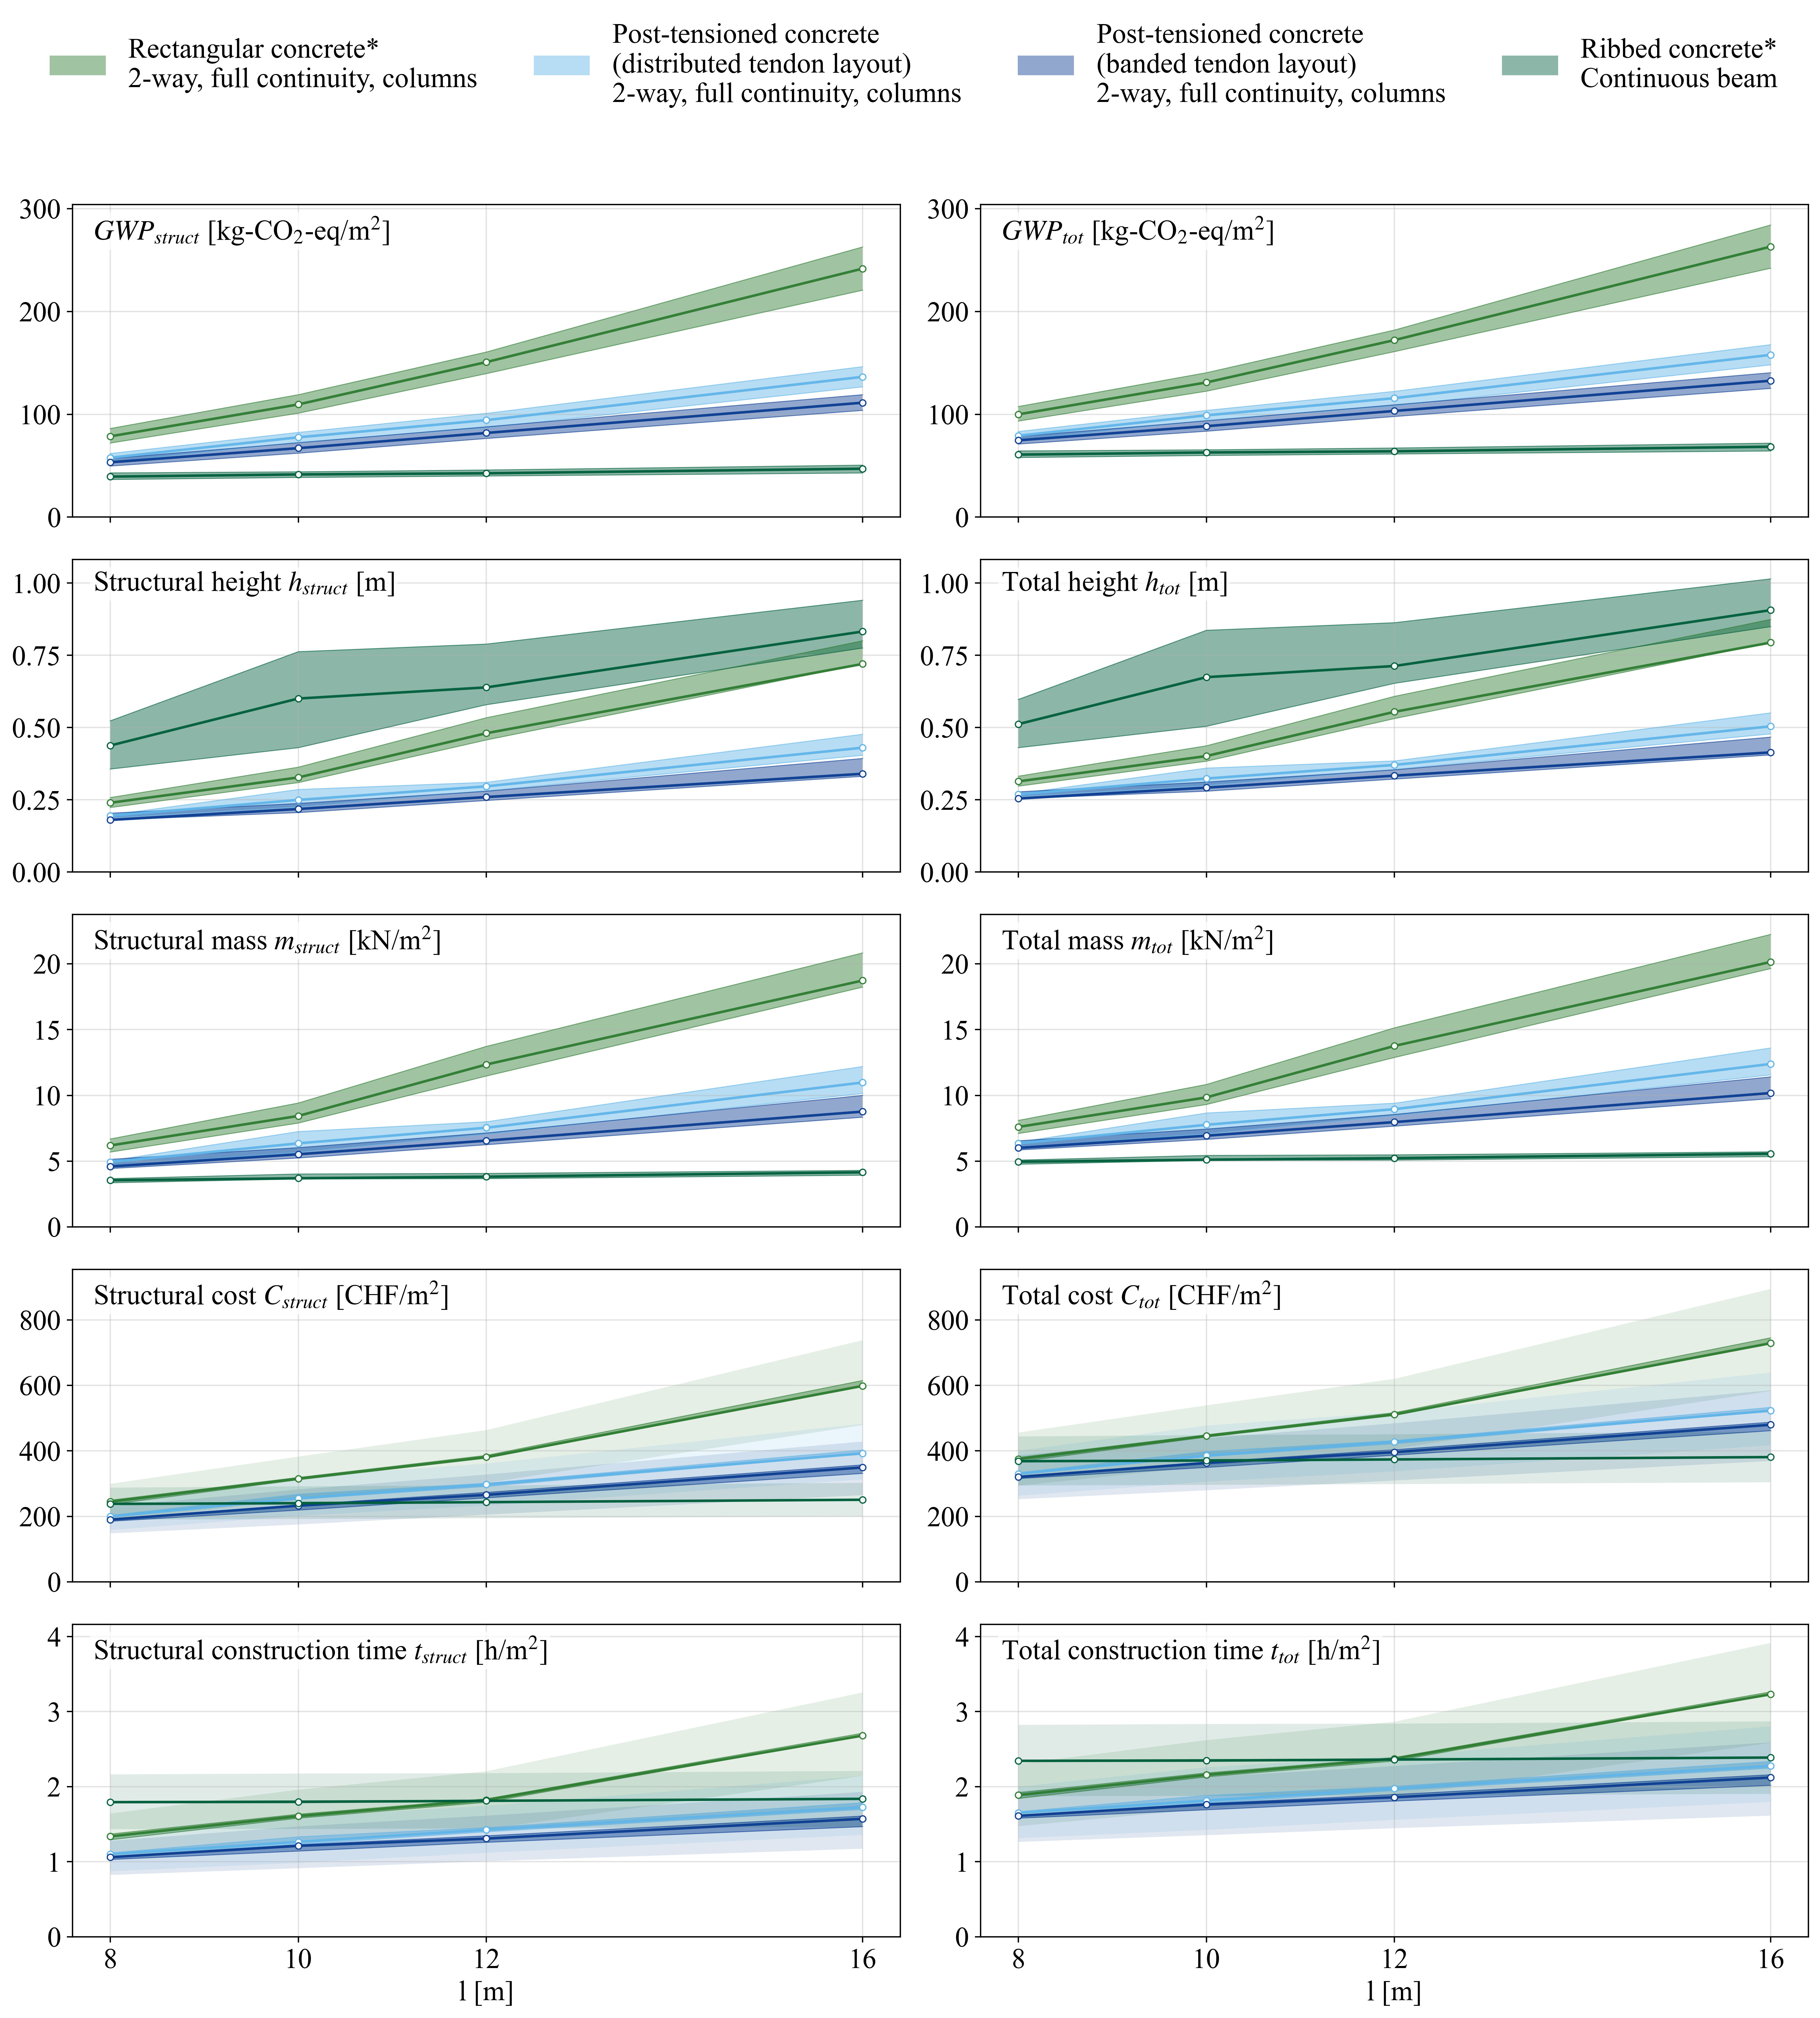
\includegraphics[width=1\textwidth]{IMAGES/final_env_comparison_office.png}
    \caption{Comparison according to sustainability assessment criteria of selected floor systems for office buildings.}
    \label{fig:final_env_comparison_office}
\end{figure}

In contrast to the residential case, only concrete-based systems are considered for the office case. Therefore, the distinction between the structural cross-section and the total floor system is less pronounced, since no comparatively heavy acoustic timber floor build-ups are required. The comparison is thus mainly governed by the structural efficiency of the concrete systems, the influence of post-tensioning, and the additional formwork demand of ribbed concrete.

\begin{figure}[H]
    \centering
    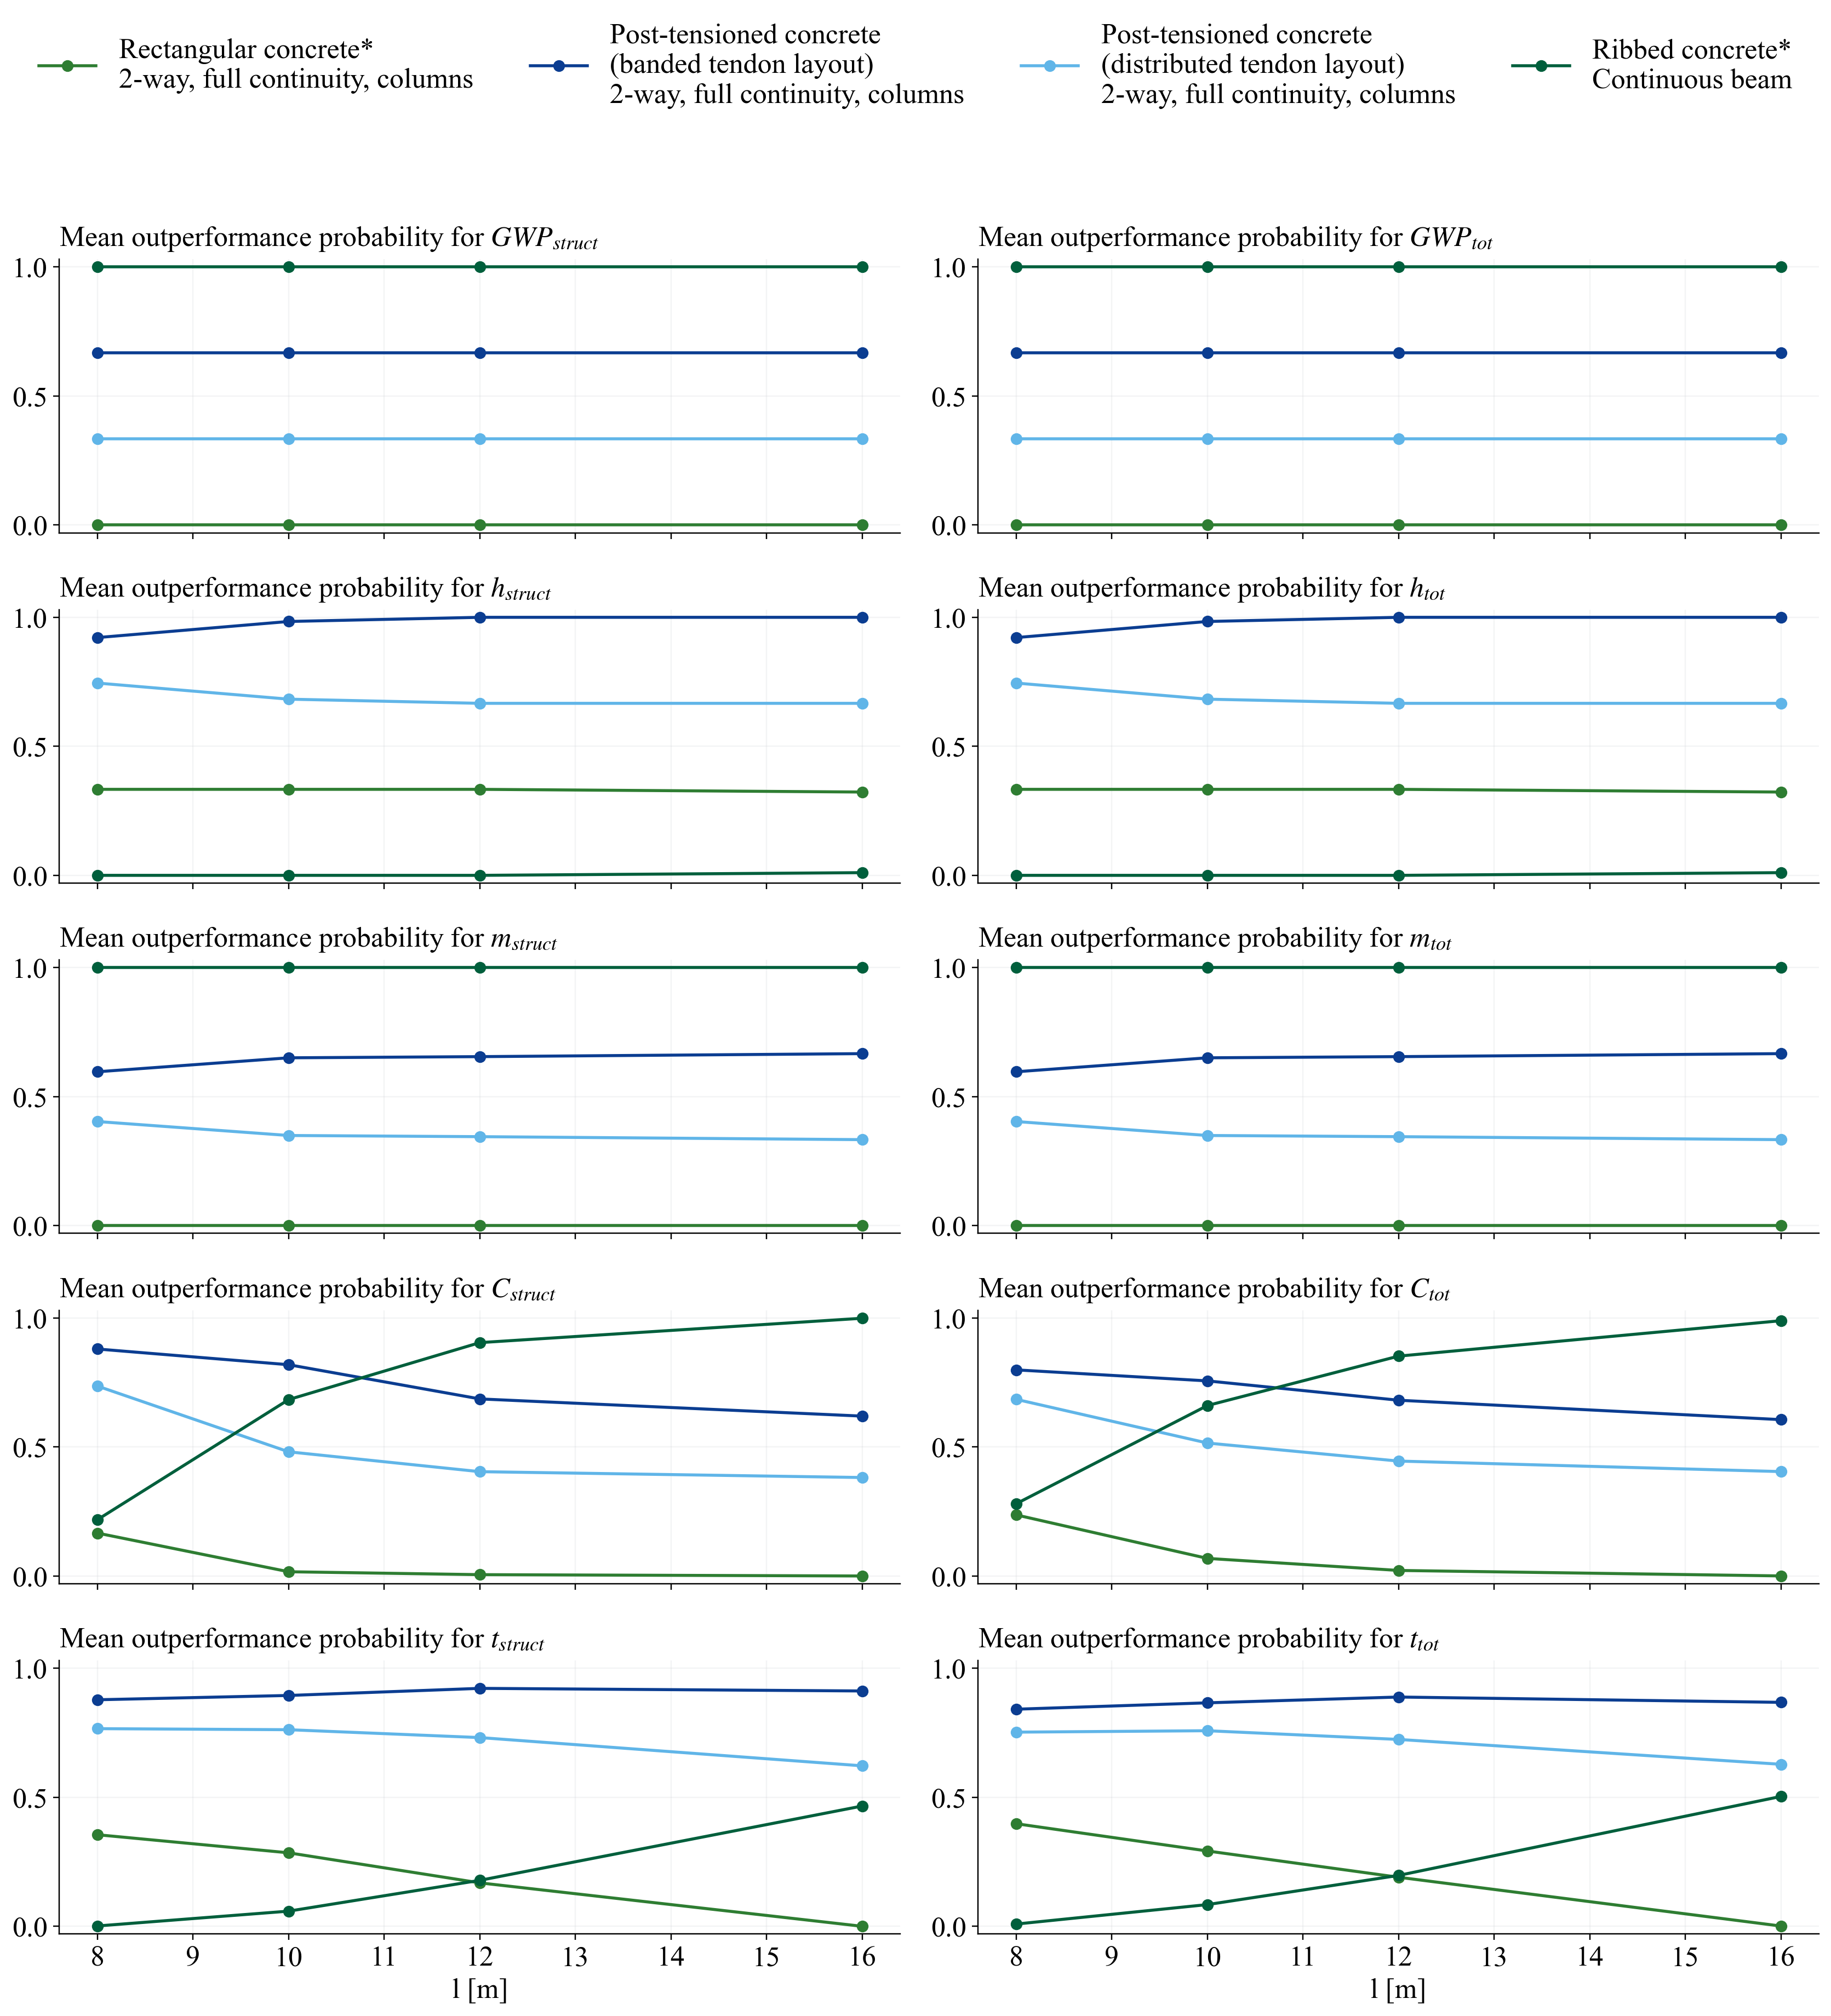
\includegraphics[width=1\textwidth]{IMAGES/uq_pairwise_scores_Office.png}
    \caption{Pairwise comparison according to sustainability assessment criteria of selected floor systems for office buildings.}
    \label{fig:uq_pairwise_scores_Office}
\end{figure}


\subsubsection{Global warming potential}

In Figure~\ref{fig:final_env_comparison_office}, ribbed concrete achieves the lowest \(GWP_{struct}\) over the investigated span range. This is also reflected in Figure~\ref{fig:uq_pairwise_scores_Office}, where ribbed concrete ranks favourably in the pairwise comparison for structural GWP. The reason is the efficient ribbed cross-section geometry, which reduces the self-weight of the cross-section while retaining sufficient bending stiffness and resistance.

Post-tensioned concrete becomes increasingly competitive with span. Compared with rectangular reinforced concrete, both post-tensioned layouts show a lower increase in \(GWP_{struct}\) over the span range. The banded tendon layout performs particularly well in the present model because the tendons are concentrated in the support strips, where the ULS checks are performed. Beneficial secondary support moments therefore reduce the governing negative support demand more effectively than in the distributed tendon layout. This effect is heavily influenced by the calculation model and must be analysed further. However, it can be hypothesised that the banded layout is a structural optimisation for post-tensioned systems and supports literature that assumes it to be a feasible post-tensioning layout \cite{PTI2023}.

Rectangular reinforced concrete shows the strongest increase in \(GWP_{struct}\) with span. This reflects the increasing slab thickness and reinforcement demand required to satisfy ULS bending. It is increasingly outperformed by post-tensioned and ribbed systems at spans above \(8\,\mathrm{m}\), aligning well with literature \cite{Rombach2010}.

\subsubsection{Height}

Figure~\ref{fig:final_env_comparison_office} shows that the post-tensioned systems achieve the lowest construction height across the investigated span range. Conventionally reinforced rectangular concrete remains competitive up to spans of \(10\,\mathrm{m}\), but then increases considerably in height, reaching values close to ribbed concrete. This is attributed to the inefficient use of material in a solid rectangular cross-section with a poor bending stiffness in relation to the self-weight.

Ribbed concrete requires a larger construction depth than the solid slab systems. Its low \(GWP_{struct}\) is therefore achieved at the cost of increased floor height. The relevance of floor height can again be illustrated using the regular building zone of the City of Zurich, where the maximum building height is limited to \(25\,\mathrm{m}\) \cite{StadtZuerich_Bauordnung_700100}.

Assuming an office room height of \(2.7\,\mathrm{m}\), the required floor depth directly affects the possible number of storeys. For a span of \(12\,\mathrm{m}\), the investigated ribbed concrete solution would allow seven storeys, whereas the post-tensioned concrete solution would allow eight storeys within the same building height. The height criterion can therefore directly influence the achievable usable floor area and should be analysed carefully.

\subsubsection{Mass}

The mass comparison follows the cross-section efficiency of the members. Ribbed concrete achieves the lowest mass as concrete is removed from structurally less effective zones of the cross-section. 

Post-tensioned concrete reduces the required concrete and reinforcement quantities compared with rectangular reinforced concrete, especially at longer spans. Therefore, it shows a more favourable mass development over the span range. Rectangular reinforced concrete becomes increasingly heavy at larger spans due to the rising demand for slab thickness and reinforcement.

Since all compared office systems require a comparable floor build-up, the differences in structural floor mass are also observed for the total cross-sections. Thus, the relevance of mass is rated higher for office buildings than for residential buildings. First, the differences between the compared systems are larger. Second, larger building envelopes are assumed for office buildings, which influence the magnitude of indirect effects on columns, foundations and lateral load-resisting systems.

\subsubsection{Construction cost}

Rectangular reinforced concrete remains economically attractive at shorter spans due to its simple geometry, established construction process, and low material cost. However, its cost increases with span as the required concrete volume and reinforcement demand increase.

Post-tensioned concrete is the most economical system for spans between approximately \(8\) and \(10.5\,\mathrm{m}\). The additional cost of tendons, anchorages, and post-tensioning operations is compensated by the reduced concrete volume and lower reinforcement demand compared with conventionally reinforced concrete. At longer spans, ribbed concrete becomes increasingly competitive because its efficient cross-section reduces material quantities. At shorter spans, however, this advantage is partly offset by the additional formwork effort caused by the ribbed geometry.

Overall, the cost performance is less pronounced than the structural GWP performance. The pairwise comparison shows that the banded post-tensioned slab has the highest total score across the investigated office span range. Ribbed concrete ranks best for \(GWP_{tot}\) and mass at all office spans and also becomes the most robust cost option from \(12\,\mathrm{m}\), but its larger construction height and longer construction time reduce its total pairwise score. The results therefore support post-tensioned concrete as the most robust overall office solution, while ribbed concrete should be selected when GWP or mass are prioritised and additional floor depth is acceptable.

\subsubsection{Construction time}

Post-tensioned concrete shows the shortest construction time across the investigated span range. The model therefore indicates that the additional process complexity of post-tensioning is offset by the reduced material demand.

Rectangular reinforced concrete shows a strong increase in construction time with span. This is mainly caused by the increasing material volume and reinforcement demand required to satisfy the structural and serviceability criteria. The heavier cross-sections at longer spans therefore directly translate into higher construction effort.

Ribbed concrete is initially penalised by the more complex formwork geometry. For spans larger than \(12\,\mathrm{m}\), the reduced material use increasingly compensates for this initial complexity, making ribbed concrete also competitive in terms of construction time.

\newpage
\section{GWP--cost correlation}
\label{sec:gwp_cost_relationship}

A conflict between GWP and construction cost is often reported in the literature \cite{Ammann2024}. In the present results, this conflict is mainly observed in the residential case, as shown in Figure~\ref{fig:scatter_gwp_total_vs_cost_total_by_case}. Based on the pairwise comparison, rectangular timber outperforms the other systems regarding \(GWP_{tot}\) at shorter spans, but it does not outperform them regarding total cost. Rectangular reinforced concrete shows the opposite tendency: it is robust regarding cost and construction height at short and intermediate spans, but it does not provide the lowest \(GWP_{tot}\). Flat TCC and ribbed TCC therefore become important compromise solutions. Flat TCC performs well when the total system is assessed across several criteria, while ribbed TCC becomes the strongest residential option at the longest investigated span.

The pairwise comparison is important because the deterministic lowest-\(GWP\) solution is not necessarily the most robust multi-criteria solution. In the residential case, rectangular timber is the clear overall pairwise winner only at the shortest investigated span. Flat TCC and rectangular reinforced concrete then alternately outperform the other systems in the intermediate range, depending on whether time and GWP or cost and height dominate the comparison. At the longest residential span, ribbed TCC outperforms the other systems in the total pairwise assessment, although post-tensioned concrete and flat TCC remain close alternatives.

The conflict between GWP and cost can therefore be tackled by separating the assessment into two steps. First, systems that are clearly dominated in the pairwise comparison should be excluded, since they do not robustly outperform the alternatives in any relevant criterion. Second, the remaining systems should be selected according to project-specific priorities. If low embodied carbon is the main objective, timber or TCC systems become preferable despite their higher modelled cost. If construction cost or floor height is the governing constraint, rectangular or post-tensioned concrete systems can be justified even when they show a higher \(GWP_{tot}\). For cases where no criterion is dominant, the pairwise comparison provides a transparent compromise by showing which system most consistently outperforms the alternatives across GWP, cost, height, mass and construction time.

The office case shows a different relationship. Since only concrete-based systems are compared, material efficiency affects both \(GWP_{tot}\) and \(Cost_{tot}\) in a similar direction. Ribbed concrete outperforms the other office systems regarding \(GWP_{tot}\) and mass across the investigated span range. It also becomes increasingly competitive regarding cost at larger spans. However, it does not achieve the best total pairwise result because its greater construction height and longer construction time reduce its overall robustness.

Accordingly, the banded post-tensioned concrete slab is the most robust office solution in the pairwise comparison. It does not show the lowest \(GWP_{tot}\), but it combines comparatively low GWP with lower construction height, shorter construction time and competitive cost. The office recommendation is therefore not based on the lowest environmental value alone, but on the system that most consistently outperforms the alternatives across the complete set of criteria.

Overall, the comparison shows that the relationship between \(GWP\) and construction cost depends strongly on the material scope of the design space. In the residential case, low-carbon solutions are not automatically low-cost solutions because timber and TCC systems are governed by different cost assumptions and construction processes. In the office case, where all systems are concrete-based, material efficiency becomes the common driver of both criteria. The conclusion is therefore not that one criterion can replace the other, but that their interaction must be interpreted separately for each building type and material family and should be evaluated with the pairwise comparison when defining application ranges.

The cost results for timber systems should be interpreted with particular caution. Their unit price is defined per cubic metre and implicitly includes fabrication and connection effort. This may overestimate the cost increase for larger timber cross-sections, because part of this effort is likely to be fixed or only weakly dependent on volume in practice. The timber cost model should therefore be validated against market data before deriving final economic recommendations. A further way to address the conflict is to include shadow carbon costs or project-specific carbon budgets in the decision process. This would make the environmental benefit of lower-GWP systems visible in economic terms and would allow designers to identify the point at which a higher construction cost is justified by the avoided emissions. Nevertheless, the observed difference between concrete and timber systems remains relevant, since a carbon price would likely have stronger leverage on concrete systems than on timber systems.

\begin{figure}[H]
    \centering
    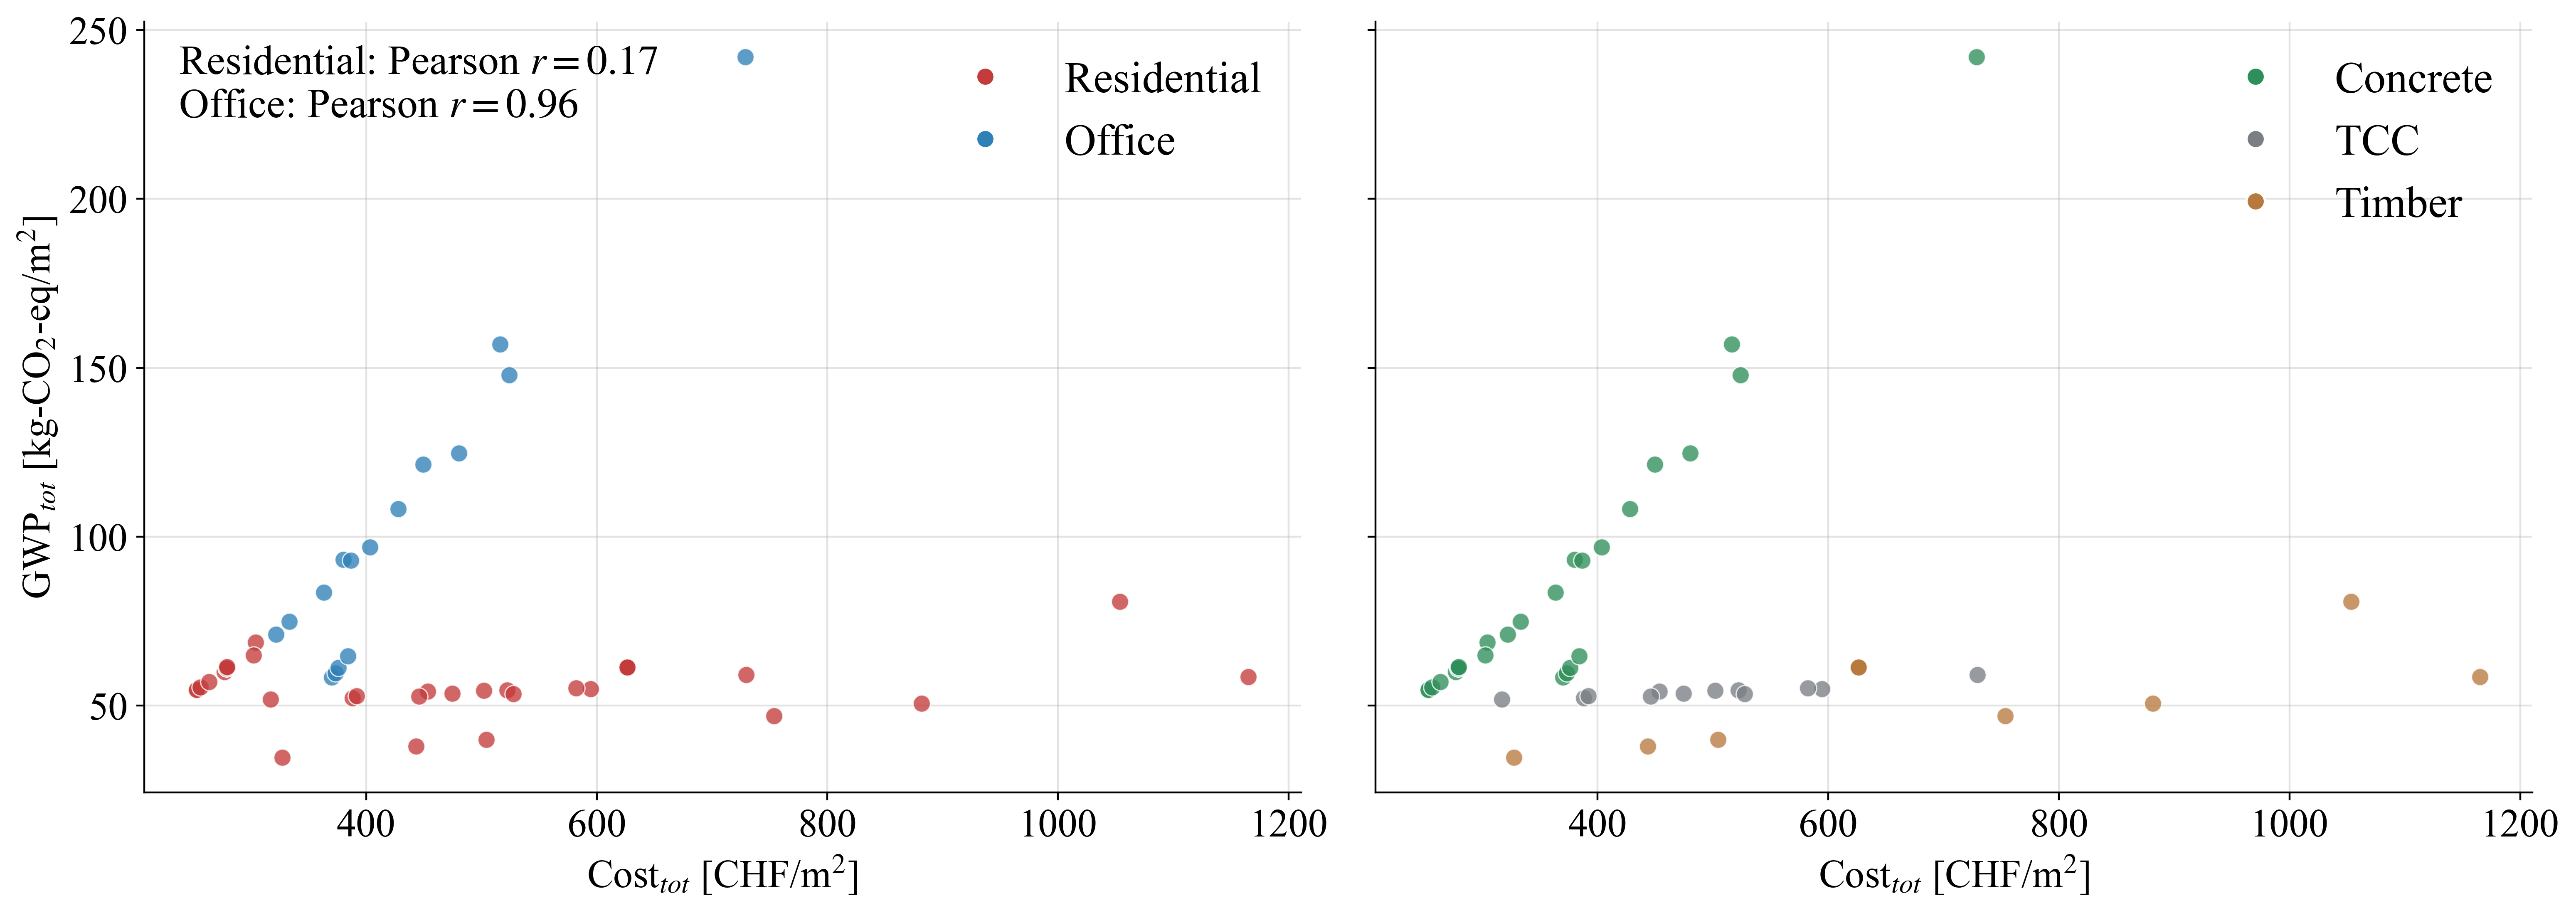
\includegraphics[width=1\textwidth]{IMAGES/scatter_gwp_total_vs_cost_total_by_case.png}
    \caption{Scatter plots between \(GWP_{tot}\) and \(Cost_{tot}\).}
    \label{fig:scatter_gwp_total_vs_cost_total_by_case}
\end{figure}


\newpage
\chapter{Conclusion}\label{chap:Conclusion} \markright {\thechapter~Conclusion}

\section{Sustainability assessment criteria}
The GWP and construction cost are treated as primary assessment criteria for sustainability to respect the ecological and the economical dimensions.

It was observed, that for concrete systems, ecological better performing systems also became economically valid. Showing that initial complexity for concrete structures does pay-off generally for spans above $7m$.

Construction height is also identified as a primary criterion, as it can directly affect the number of possible storeys within a fixed building envelope and therefore influence the usable floor area. 

Mass is considered a secondary criterion for residential buildings, since acoustic floor build-ups reduce the differences in total system weight. For office buildings, mass is more relevant because the total weight is governed more directly by the structural cross-section.

Construction time is important, but project-dependent. It may become a primary criterion when prefabrication, short construction periods or reduced propping times are central to the project strategy.


\section{Slab systems for residential buildings}
No system performs best across all criteria and spans. Rectangular timber is favourable for short spans because of its low structural GWP and mass, although its cost and required height increase at longer spans. Rectangular concrete provides a balanced solution at intermediate spans, combining low cost and construction height with competitive GWP.

At longer spans, post-tensioned concrete provides a favourable balance of GWP, height, cost, and construction time. Ribbed TCC achieves very low structural GWP but requires substantially greater construction depth. Flat TCC offers a compromise between these alternatives through moderate depth and short construction time.

% Plot that indicates the areas of application
\begin{figure}[H]
    \centering
    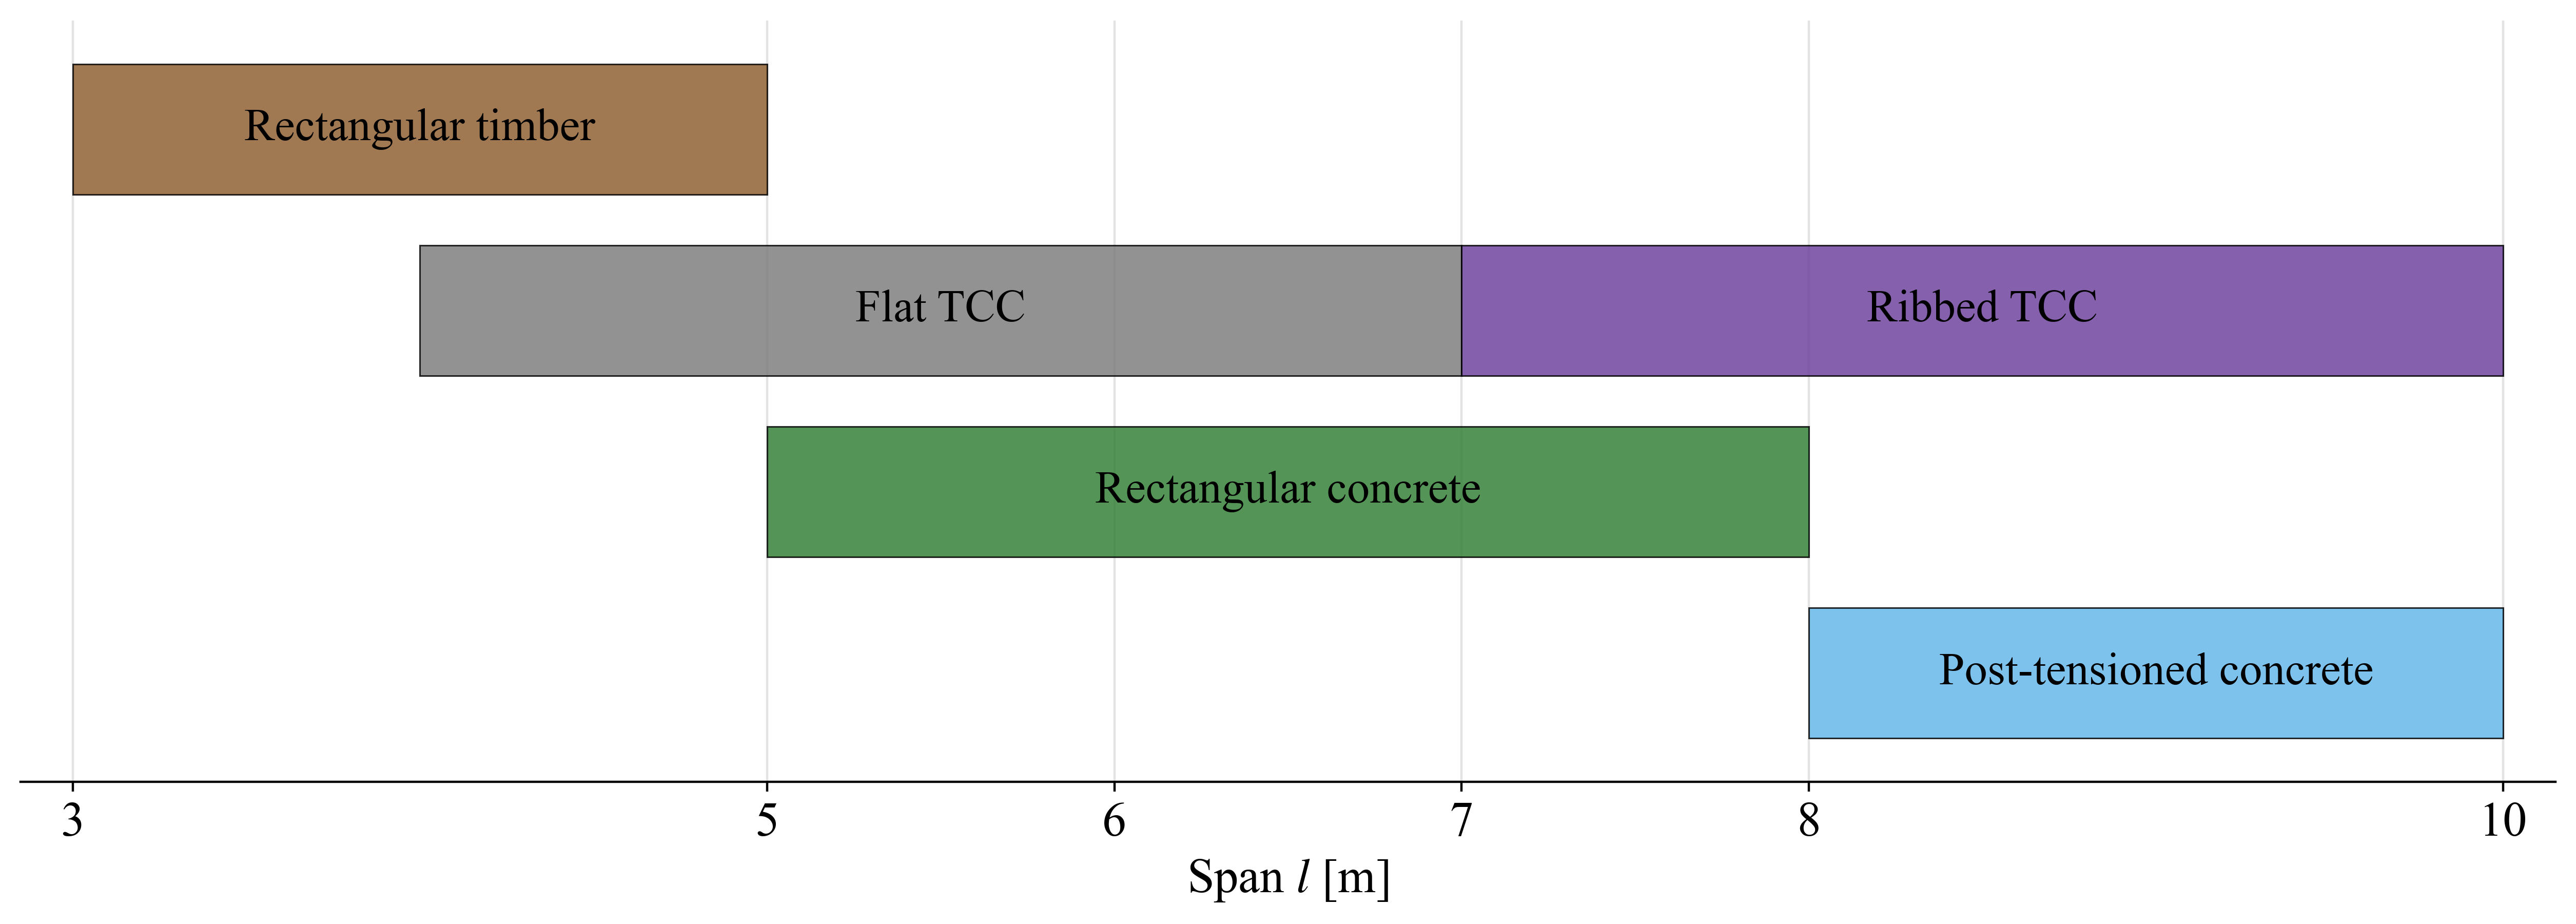
\includegraphics[width=1\textwidth]{IMAGES/final_application_ranges_residential.png}
    \caption{Proposed application ranges by span of compared systems for residential builings.}
    \label{fig:final_application_ranges_residential}
\end{figure}

The ribbed timber hollow-core system is lightweight but performs poorly regarding GWP and cost under the present assumptions. Its simplified fire verification and sensitivity to the selected insulation demonstrate the limitations of the configurator for highly specialised systems. More detailed fire checks and manufacturer-specific product data would be required for a conclusive assessment. As a result, the timber hollow-core system is excluded from Figure \ref{fig:final_application_ranges_residential}.


\subsection{Slab systems for office builings}
The office comparison showed that no system performs best across all criteria and spans. Rectangular reinforced concrete is not recommended for the investigated span range. It is neither economically competitive nor functionally advantageous, as its material demand, construction height, and \(GWP_{struct}\) increase strongly with span.

Post-tensioned concrete provides the best overall balance. It combines low construction height with competitive \(GWP_{struct}\) and remains economically competitive at larger spans. The banded tendon layout is recommended across the full investigated span range. It benefits from tendons concentrated in the support strips and leaves the field regions largely free for further material-saving measures, such as formwork inlays. The distributed tendon layout is recommended only when a banded layout is not possible and only up to approximately \(12\,\mathrm{m}\).

Ribbed concrete is recommended for spans from approximately \(10\) to \(16\,\mathrm{m}\), where its reduced material demand leads to favourable environmental and economic performance. However, it requires a larger construction depth and may therefore be excluded when floor height is a governing constraint.
\begin{figure}[H]
    \centering
    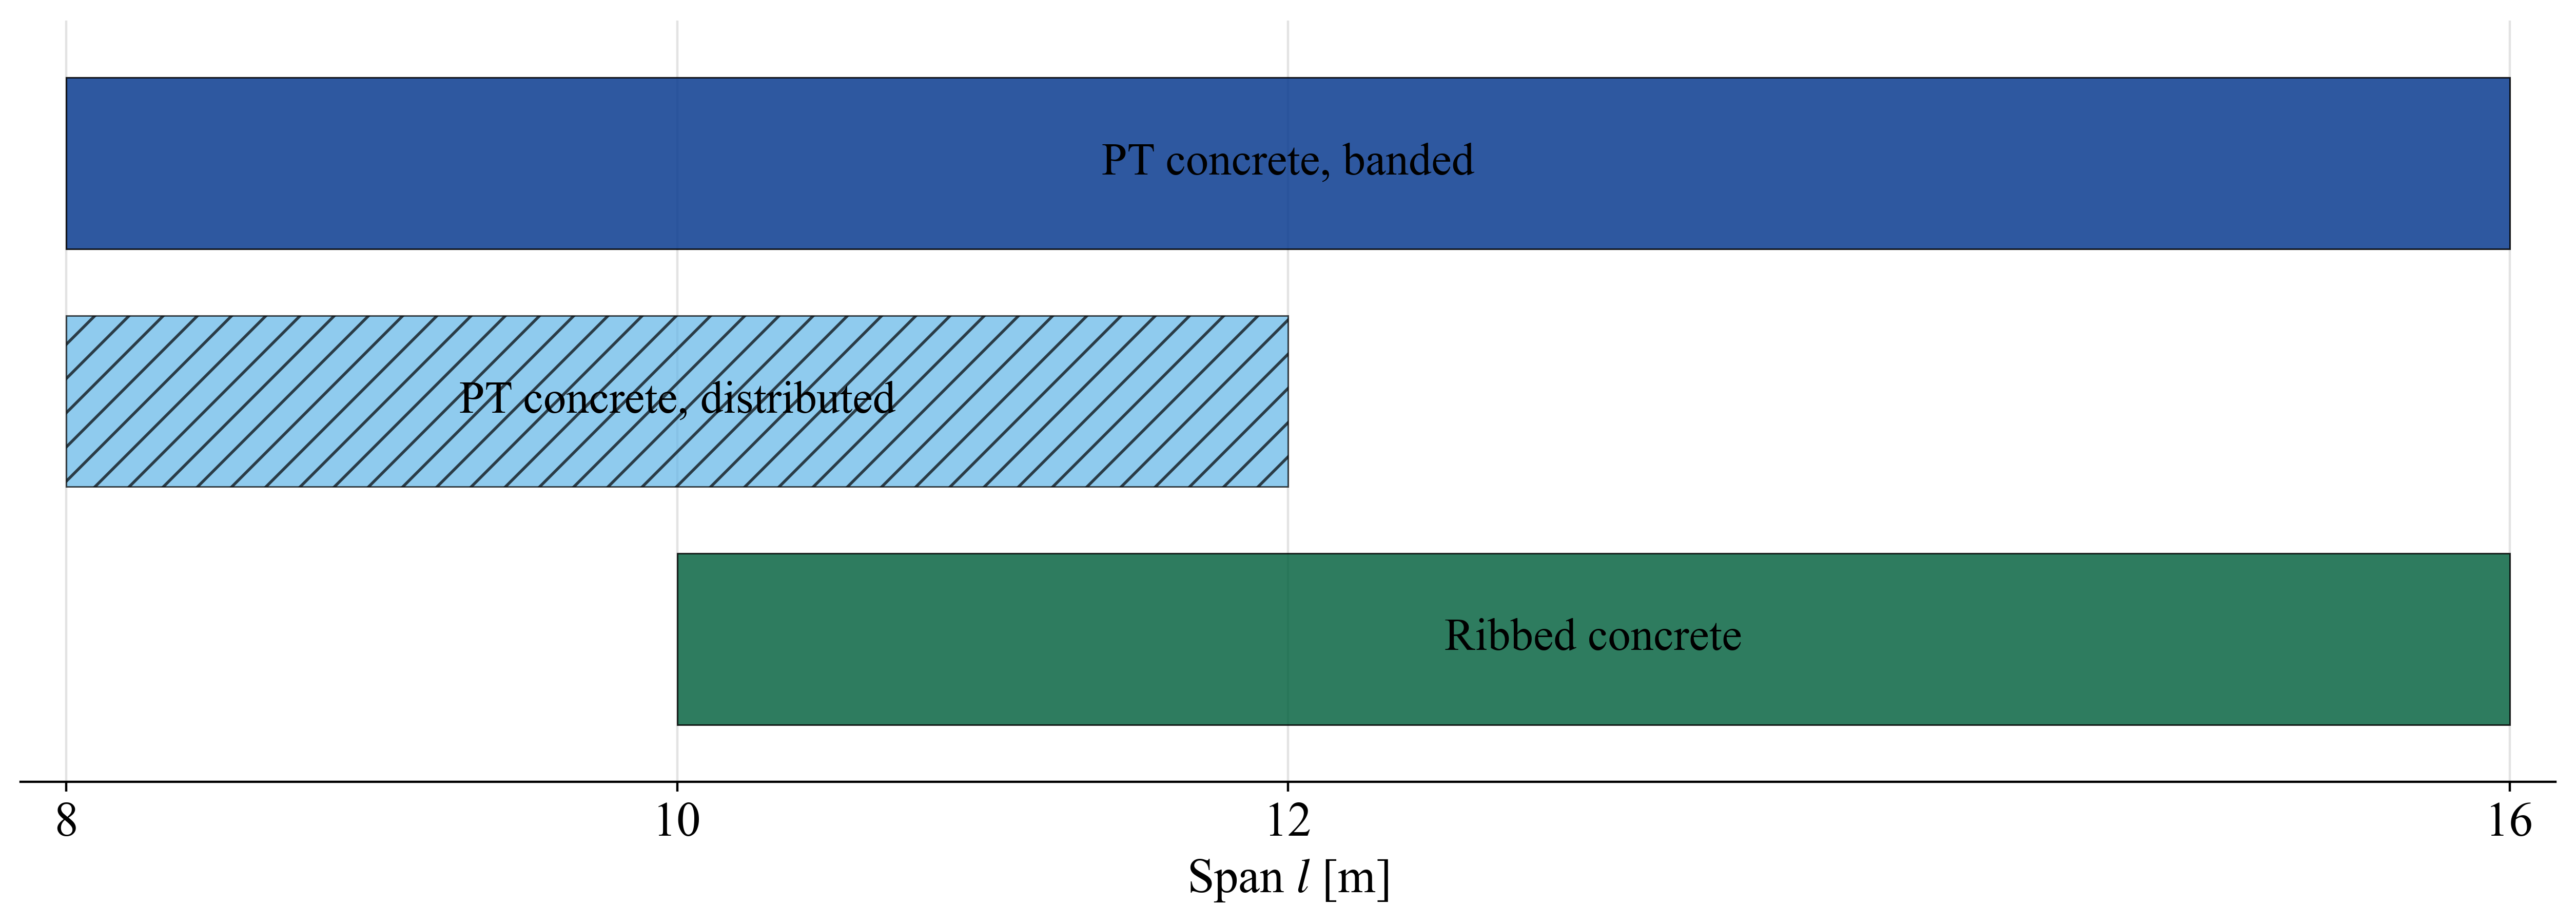
\includegraphics[width=1\textwidth]{IMAGES/final_application_ranges_office.png}
    \caption{Proposed application ranges by span of compared systems for office buildings.}
    \label{fig:final_application_ranges_office}
\end{figure}








\newpage
\chapter{Outlook}\label{chap:Outlook} \markright {\thechapter~Outlook}
Future work should extend the range of slab systems implemented in the configurator. In particular, the ribbed timber hollow-core system should be improved by considering different insulation products and by implementing a more refined fire verification. Post-tensioning could also be extended to ribbed concrete slabs, together with an improved two-dimensional structural handling. In addition, continuity effects for timber--concrete composite systems should be included, as proposed in the revised Eurocode~5 \cite{Eurocode5_2023}.

Further studies should investigate the sensitivity of the results to changed boundary conditions. This includes the effect of increased acoustic requirements that can be already handled, as well as higher imposed and permanent loads. Such analyses would help to identify how robust the observed system rankings are under different design assumptions.

Finally, the method should be made more accessible for practising engineers. A web-based user interface could allow users to weight the sustainability assessment criteria according to the pairwise comparison method. As a first step in this direction, a prototype website was developed that enables interactive adjustment of the criterion weights and visualises the resulting pairwise system ranking. The configurator could therefore be developed into a practical decision-making tool for early-stage design.





% Bibliography__________________________________________________________________
% Literature (Additional references can be added to the .bib-file manually, or by using, for example, the free application JabRef). 
% \makeatletter \renewcommand*{\chapterheadstartvskip}{\vspace{\dimexpr\@tempskipa-10\baselineskip}} %letzte quelle noch quetschen
%%%%%

{\scriptsize
\raggedleft
\bibliographystyle{unsrtnat}
\bibliography{bibliography}
}
%\makeatletter \renewcommand*{\chapterheadstartvskip}{\vspace{\dimexpr\@tempskipa-3\baselineskip}}
% Temporarily prevent page breaks

{\footnotesize
\listoffigures}
{\footnotesize
\listoftables}


% Anhang______________________________________________________________________
\chapter{Appendix}\label{chap:Appendix} \markright {\thechapter~Appendix}

\section{UML diagram for slab configurator system architecture}
\begin{figure}[H]
    \centering
    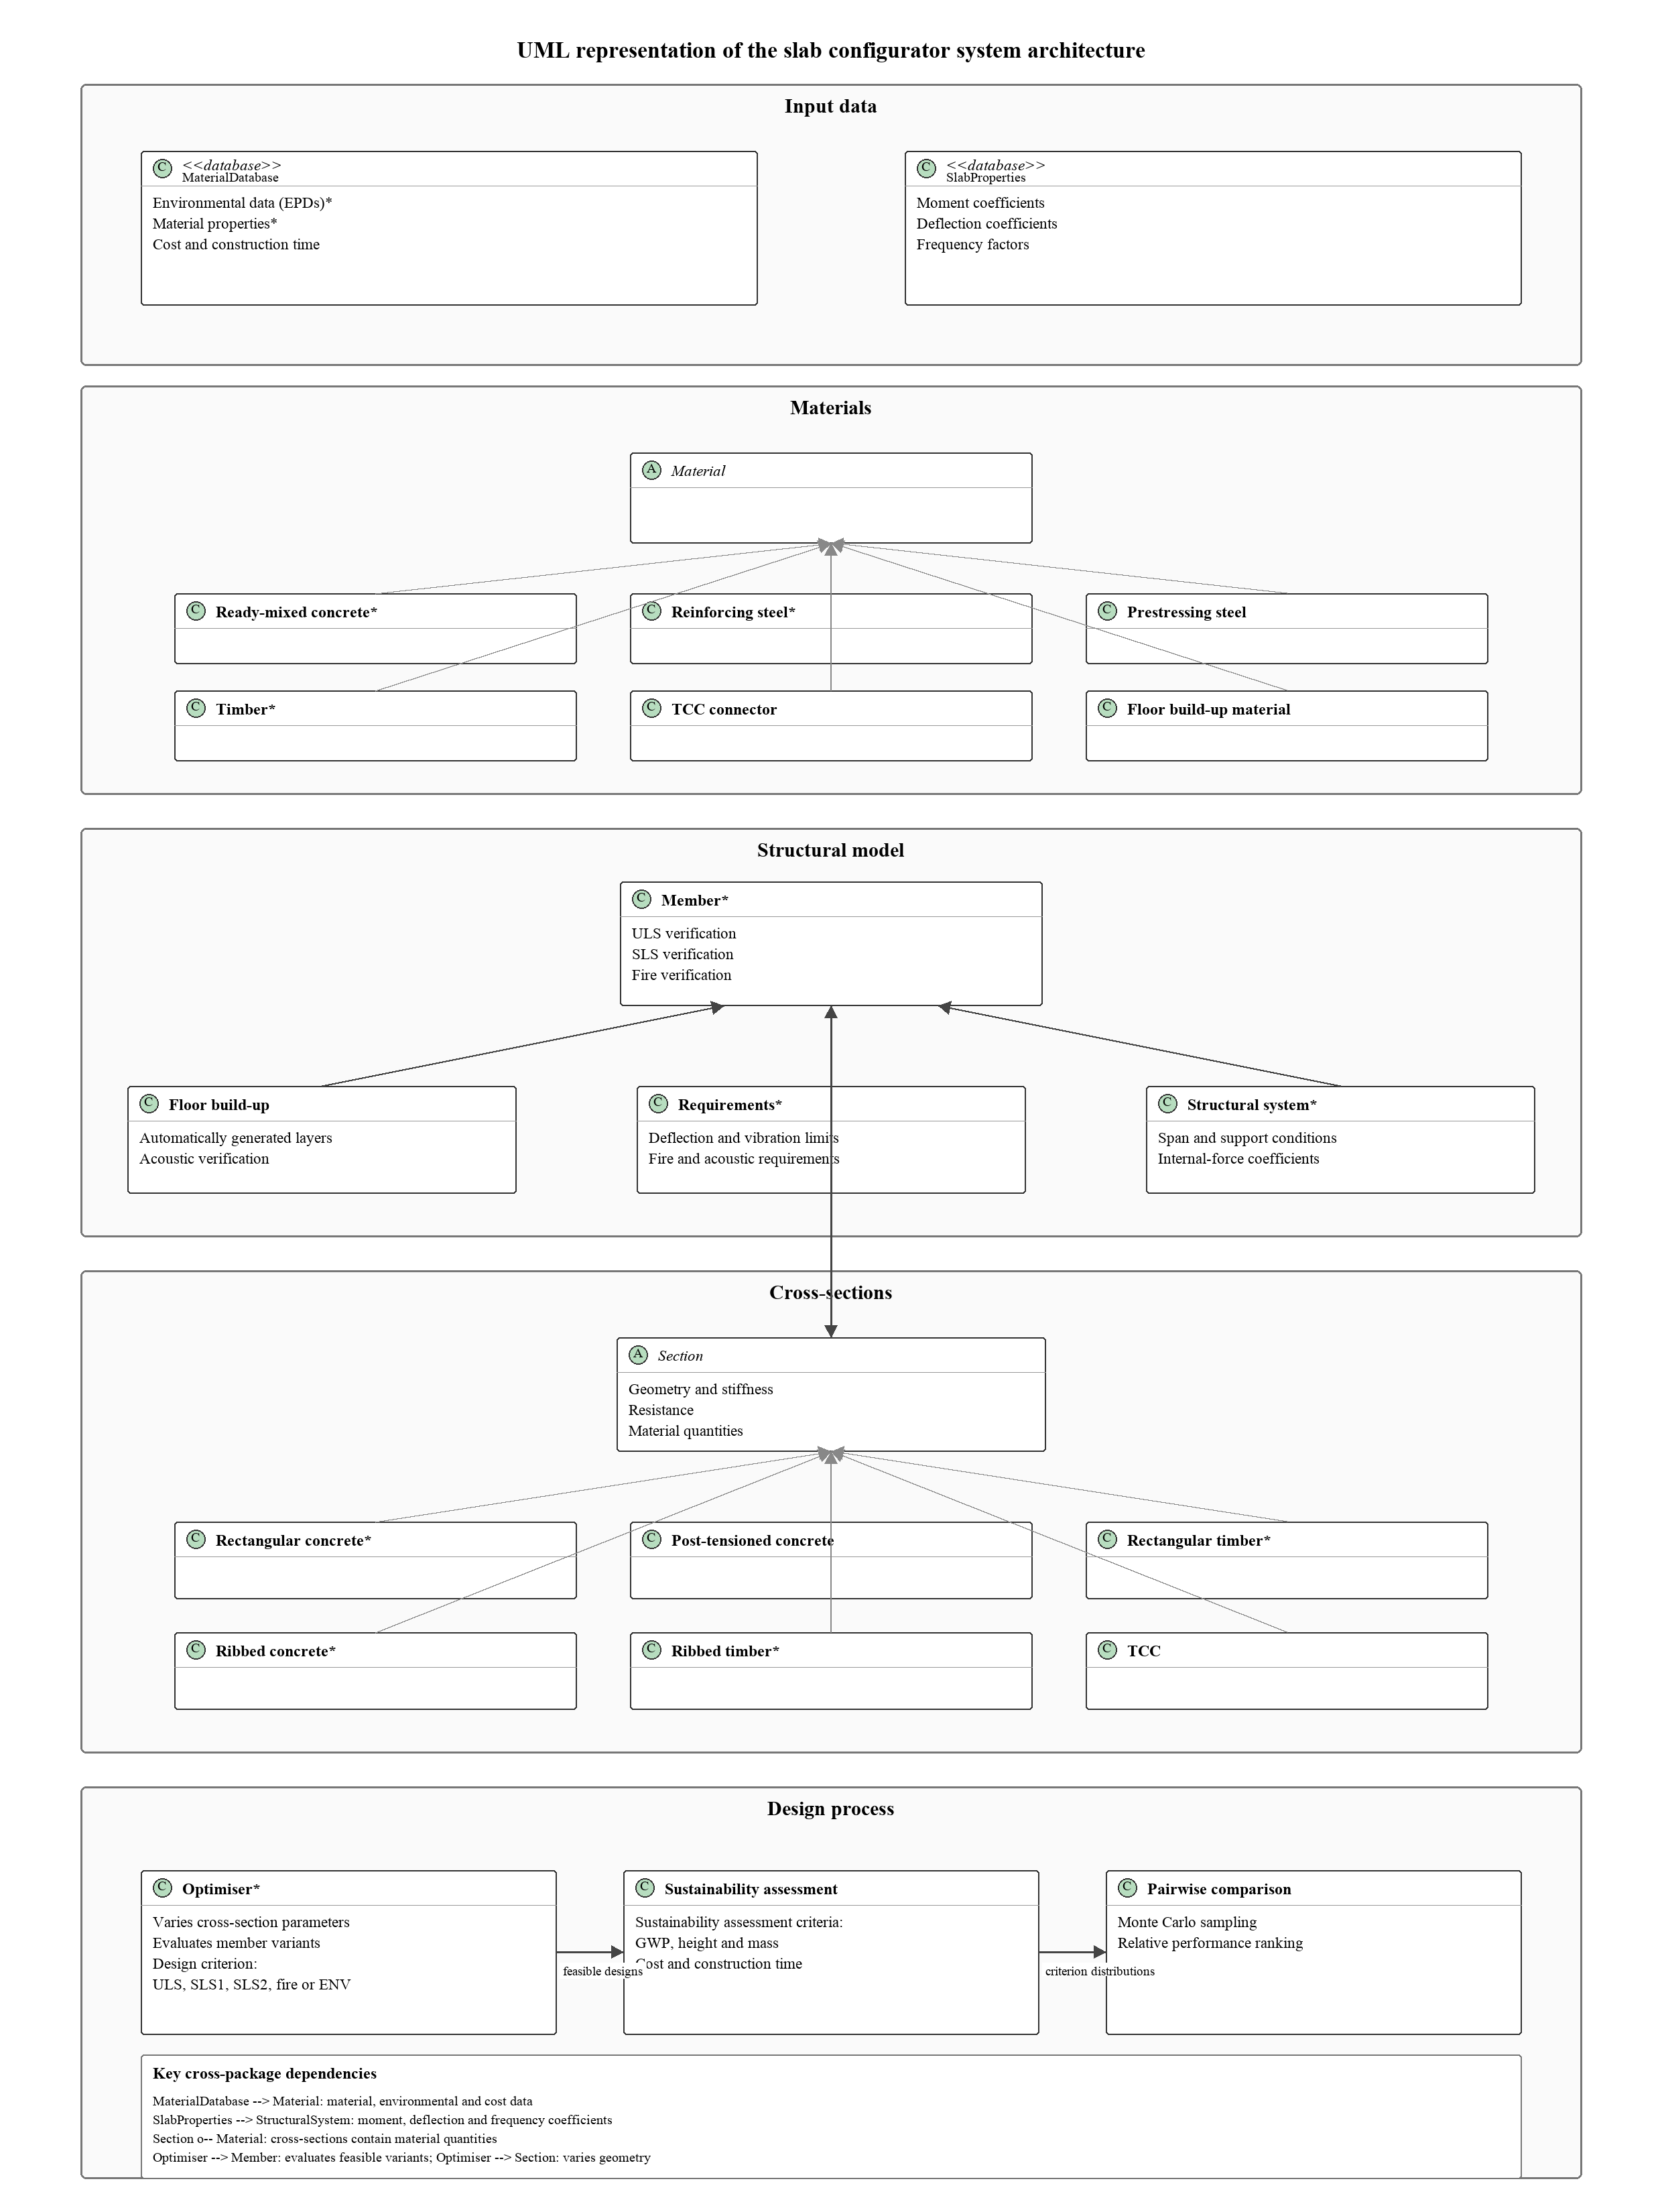
\includegraphics[width=1\textwidth]
        {IMAGES/SDSD_architecture_report.png}
    \caption{UML representation of the extended Python framework and the main
    relationships between its data sources, classes and assessment methods. (*) Denotes classes and databases that were already handled by the initial slab configurator.}
    \label{fig:software_architecture}
\end{figure}



\section{Finite-element analysis post-tensioned concrete class validation}
\begin{figure}[H]
    \centering
    \includegraphics[width=1\textwidth]{IMAGES/Druckauszug_EI_Validation.jpg}
    \caption{Validation of post-tensioned concrete class Cubus documentation. Not printed true to scale.}
    \label{fig:CubusEiVal}
\end{figure} %für umfangreiche Rohdaten oder Prozedurenbeschreibungen

\end{document}

